% Latex Beamer template following CERN template guidelines (or trying!)

\documentclass[aspectratio=169]{beamer}
\usepackage{xcolor}
\usepackage{graphicx}
\usepackage{multicol}
\usepackage{tikz}

% Code listings with syntax highlighting
%  Require Pygments
\usepackage{minted}

\usetheme{CERN}

\newcommand{\interludeTitle}{}
\AtBeginSection[] {
    \frame{
	\frametitle{\interludeTitle}
      \begin{multicols}{2}
        \tableofcontents[
            currentsection,
            sectionstyle=show/shaded,
            ]
	  \end{multicols}
    }
}

%\AtBeginSubsection[] {
%	  \frame{
%		\frametitle{\interludeTitle}
%		\begin{multicols}{2}
 %       \tableofcontents[
  %          currentsubsection,
   %         subsectionstyle=show/shaded,
%            ]
%		\end{multicols}
%	  }
%}


% Talk date
% Uncomment this to define a presentation date distinct from \today
% \def\mydate{20 Feb 2000}

% Preamble
\title[]{PS Space Charge Simulations}
\subtitle{Updates}
\author[Haroon Rafique]{\texorpdfstring{\url{haroon.rafique@cern.ch}}{Author}}

% Body
\begin{document}
    
    \cernSplashBlue

    % Title
    {
    \setbeamertemplate{footline}{}
    \setbeamertemplate{navigation symbols}{}
    \frame{\titlepage}
    }
    \setcounter{framenumber}{0}

    % TOC
    \frame{
        \frametitle{Table of Contents}
        \begin{multicols}{2}
            \tableofcontents
        \end{multicols}
    }



    \section{MD4224 Injection Bump}

    \frame{
        \frametitle{Methods Explored}
        
        At each of the four sections (40, 42, 43, 44) in the PS we use:
        
        \begin{itemize}
            \item Two 10 cm HKICKER with MULTIPOLE inbetween for the sextupole component.
            \item A single zero-length MULTIPOLE with dipolar and sextupolar components.
            \item A single 20 cm (zero gradient) QUADRUPOLE with dipolar and sextupolar components added as errors.
            \item A single 20 cm (zero angle) SBEND with dipolar and sextupolar components added as errors.
        \end{itemize}
    }
    
    \frame{
        \frametitle{Injection Bump - Closed Orbit}
        
        Start with the injection bump closure given by dipole components only.
    
    }
    
    \frame{
        \frametitle{Split HKICKER Closed Orbit}
        \begin{figure}
            \centering
            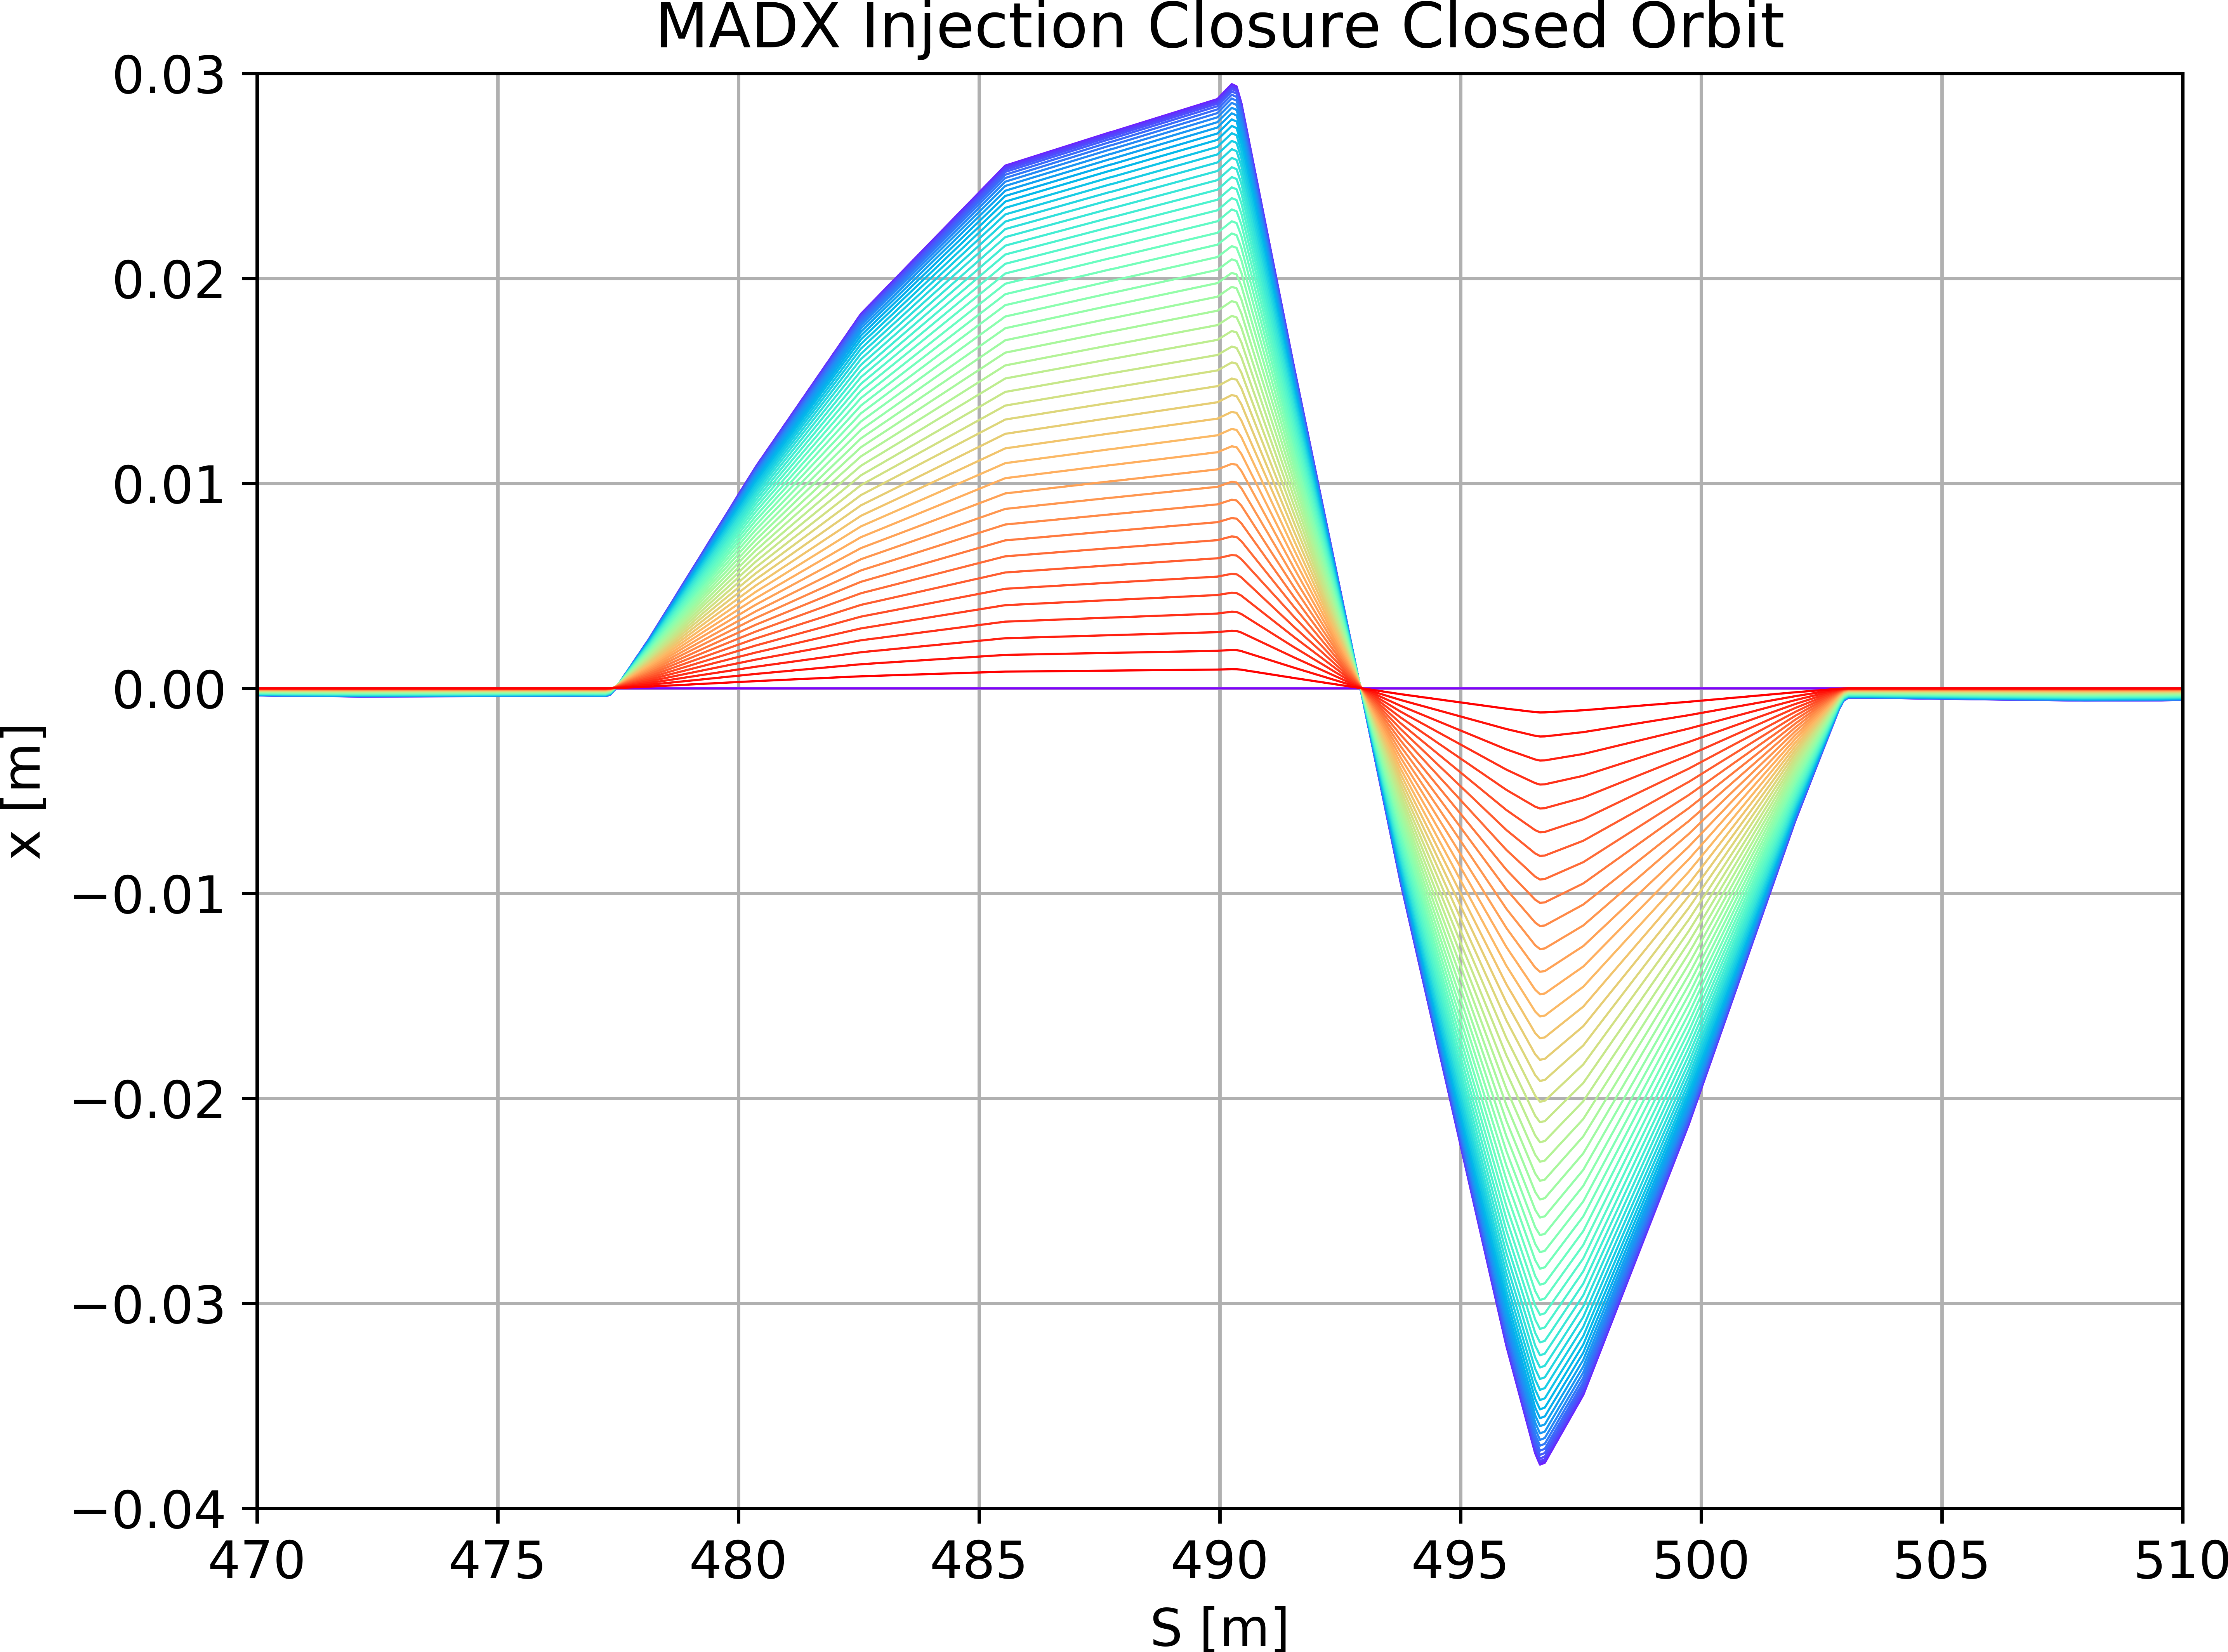
\includegraphics[width=0.3\textwidth]{No_Sext/00_HKICKER/MADX_Closed_Orbit00_Split_HKICKER_with_MULTIPOLE_zoom.png}~~~~~
            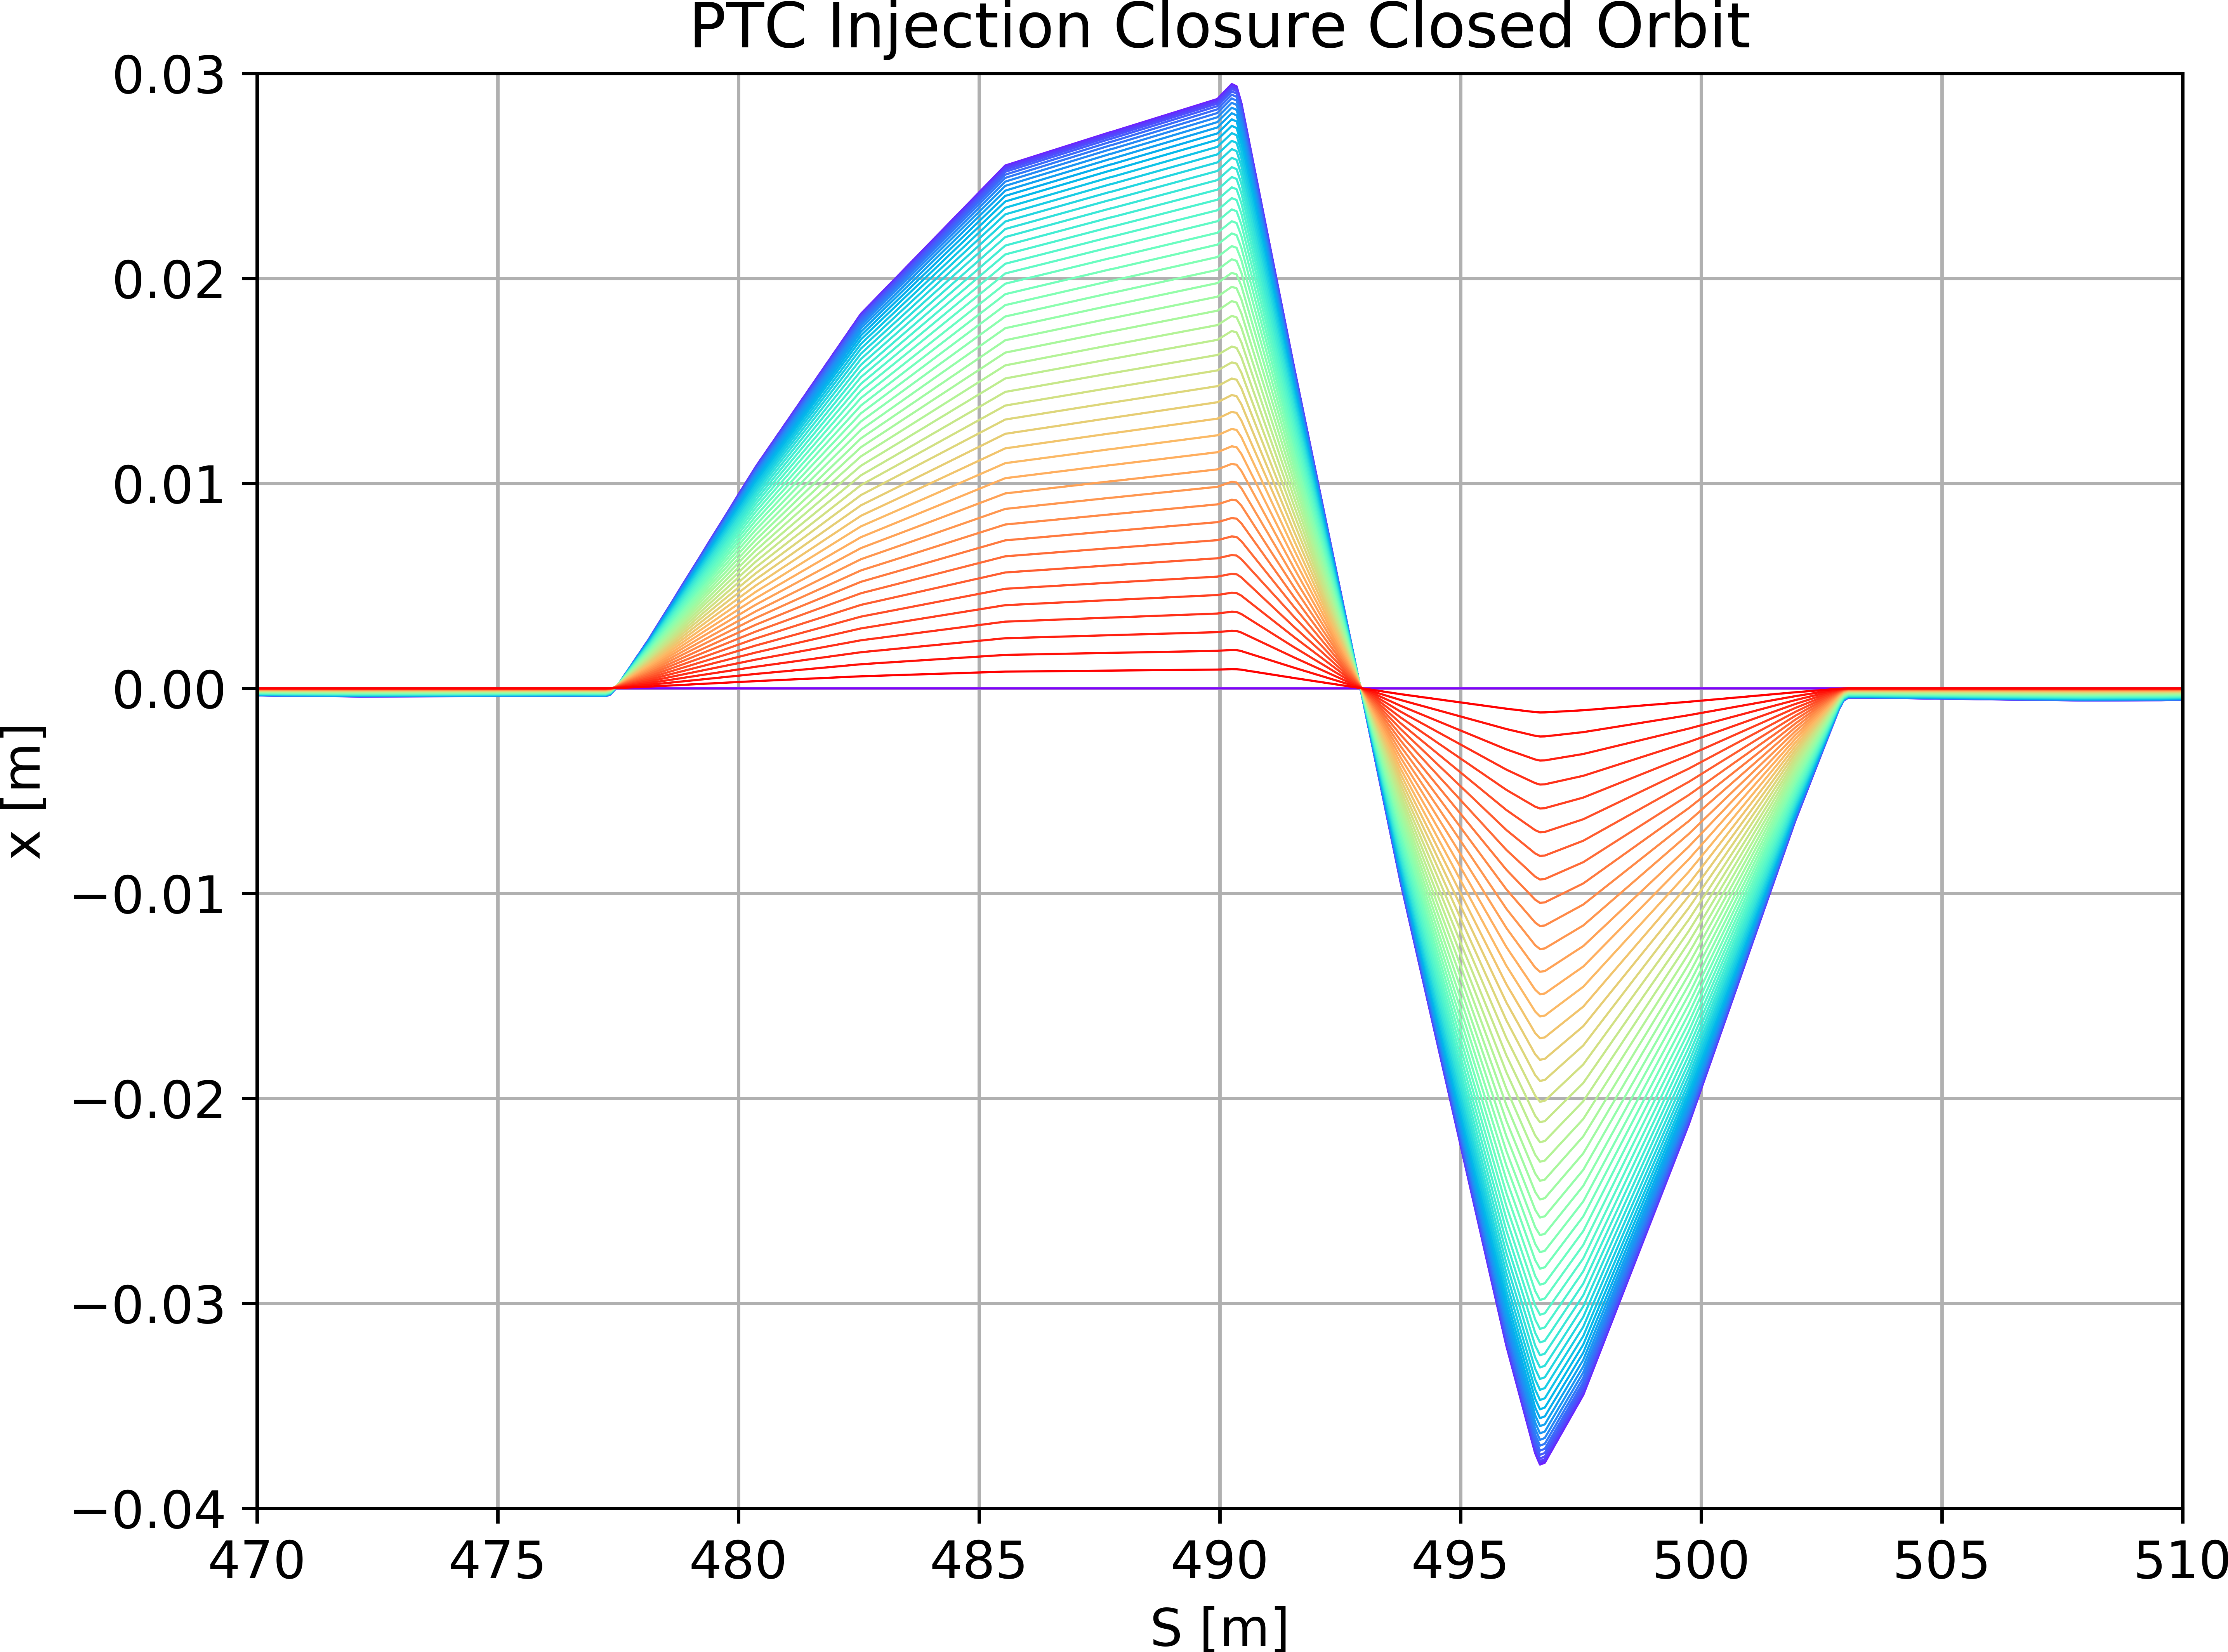
\includegraphics[width=0.3\textwidth]{No_Sext/00_HKICKER/PTC_Closed_Orbit00_Split_HKICKER_with_MULTIPOLE_zoom.png}~~~~~
            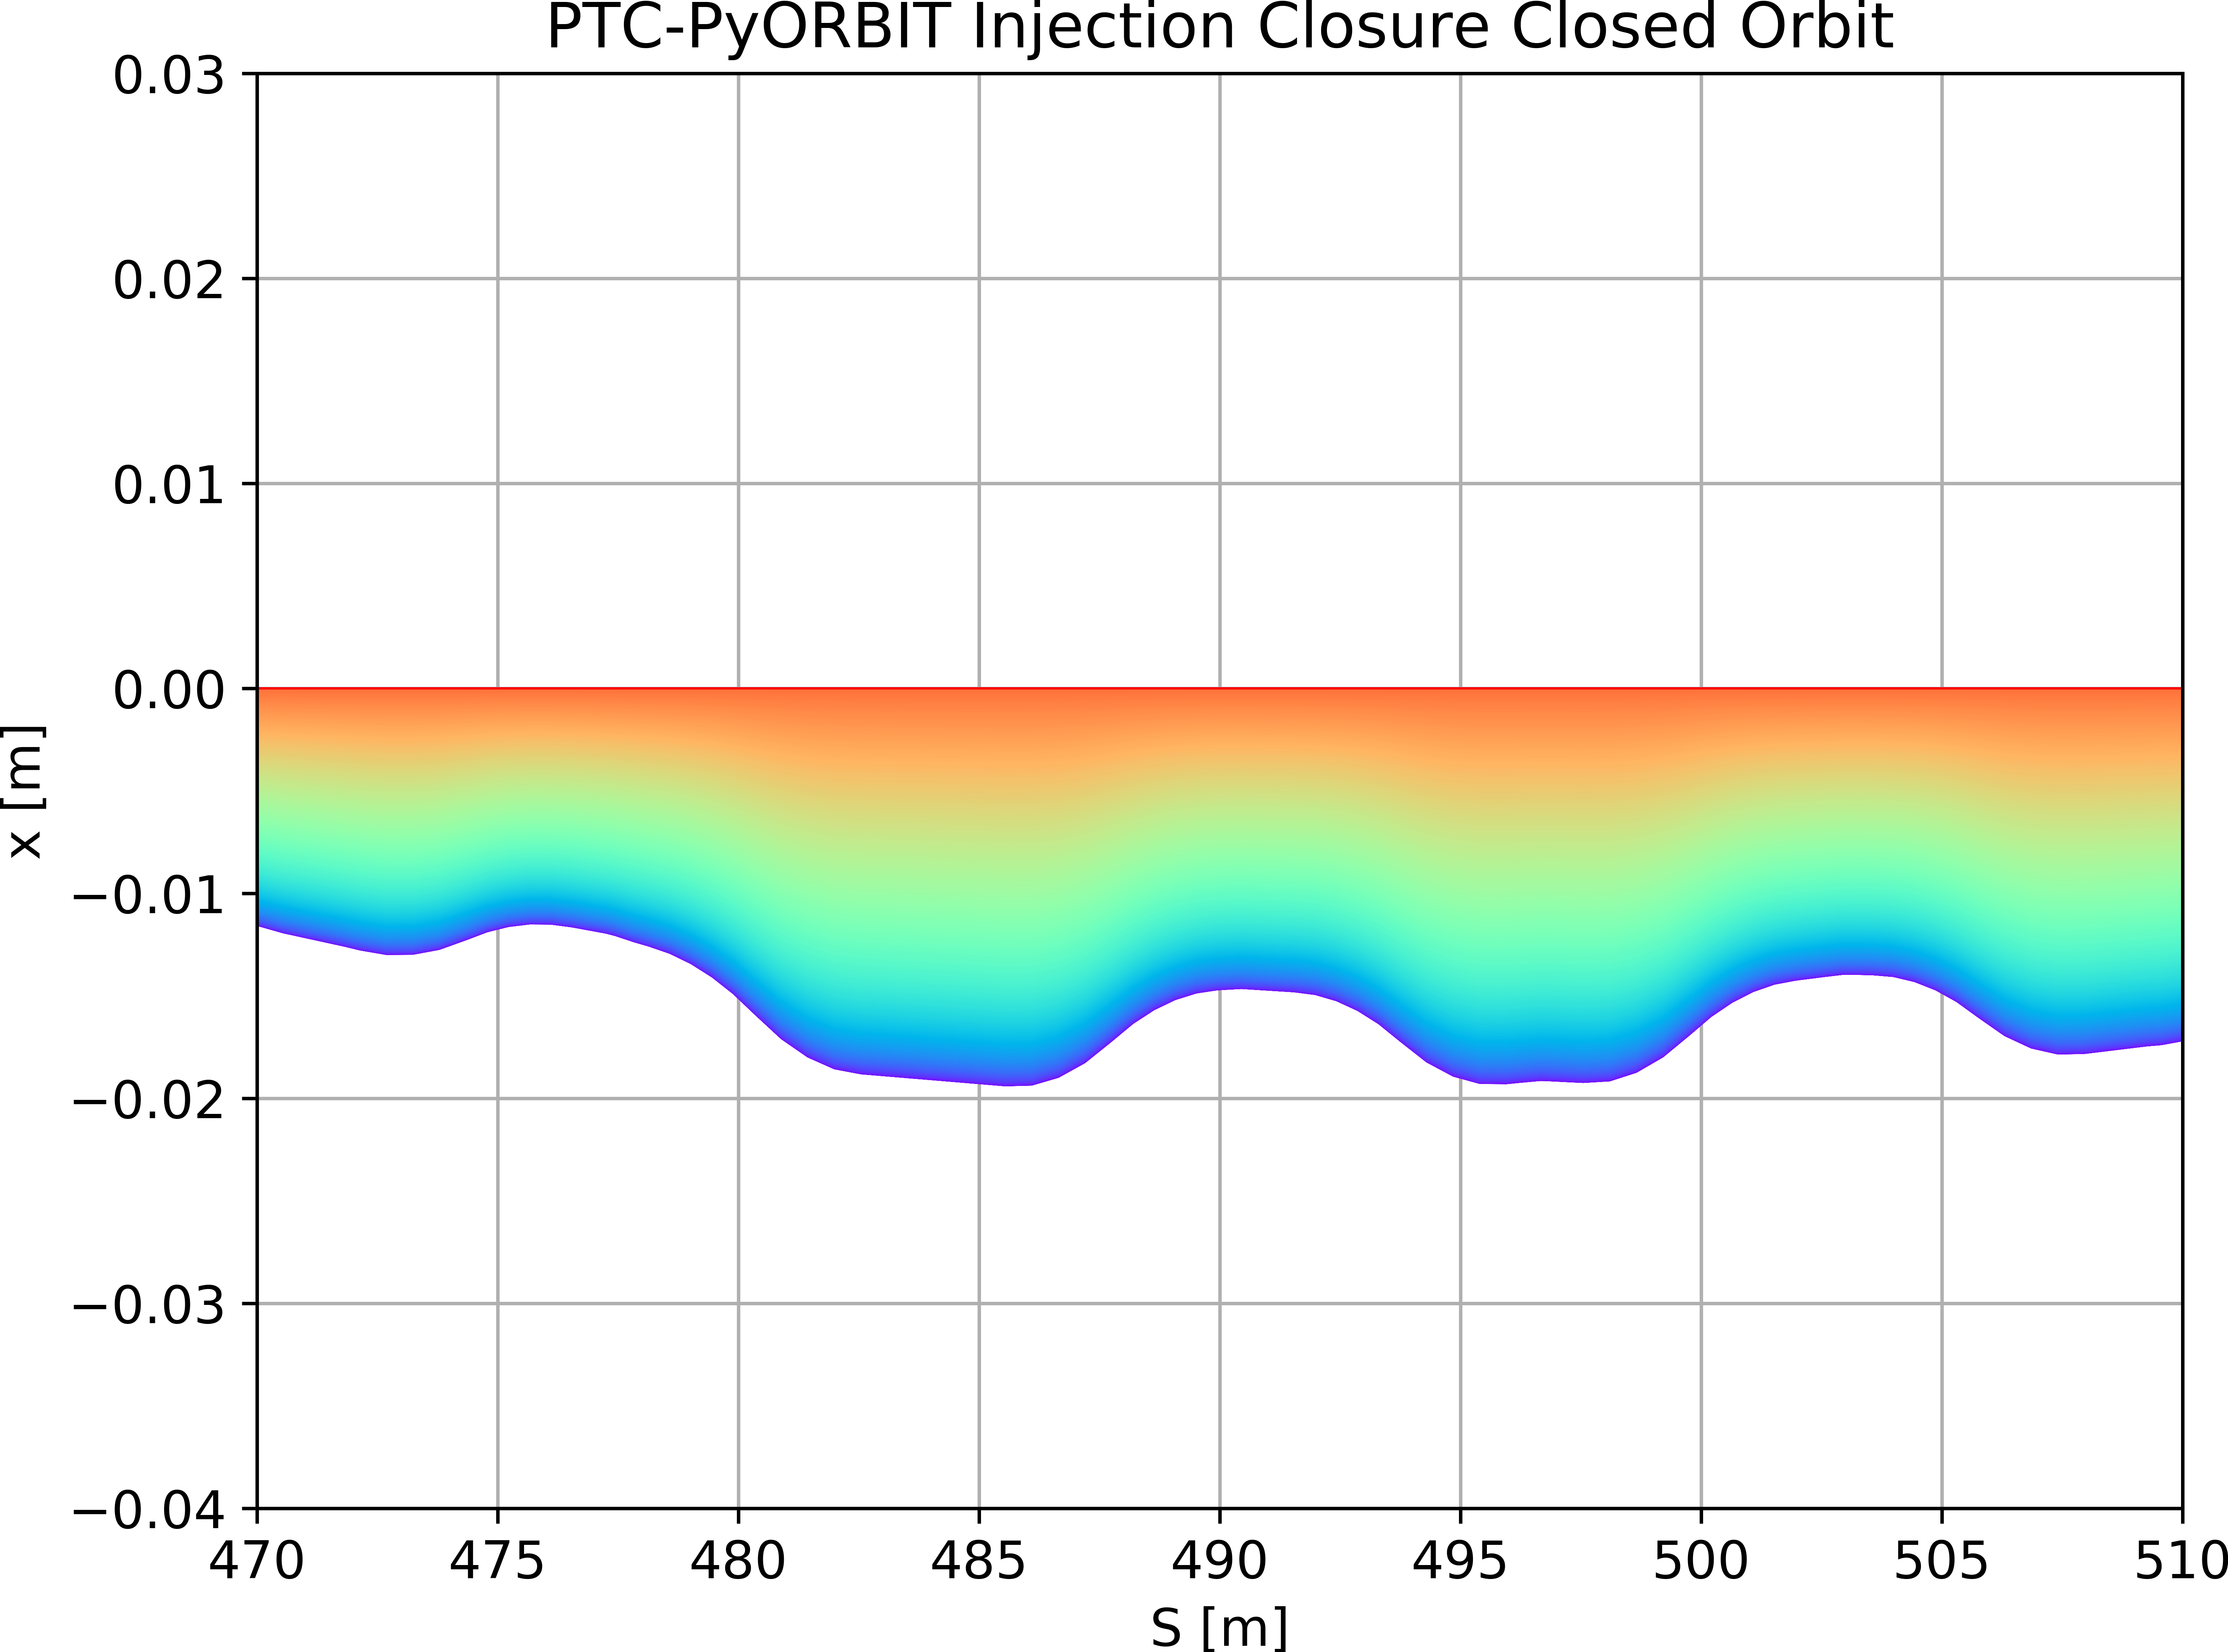
\includegraphics[width=0.3\textwidth]{No_Sext/00_HKICKER/PTC-PyORBIT_Closed_Orbit00_Split_HKICKER_with_MULTIPOLE_zoom.png}
            \caption{Horizontal closed orbit for split HKICKER + MULTIPOLE: MAD-X, PTC, PyORBIT.}
            \label{fig:00_CO_zoom}
        \end{figure}
    }
     \frame{
        \frametitle{Split HKICKER Closed Orbit}
        \begin{figure}
            \centering
            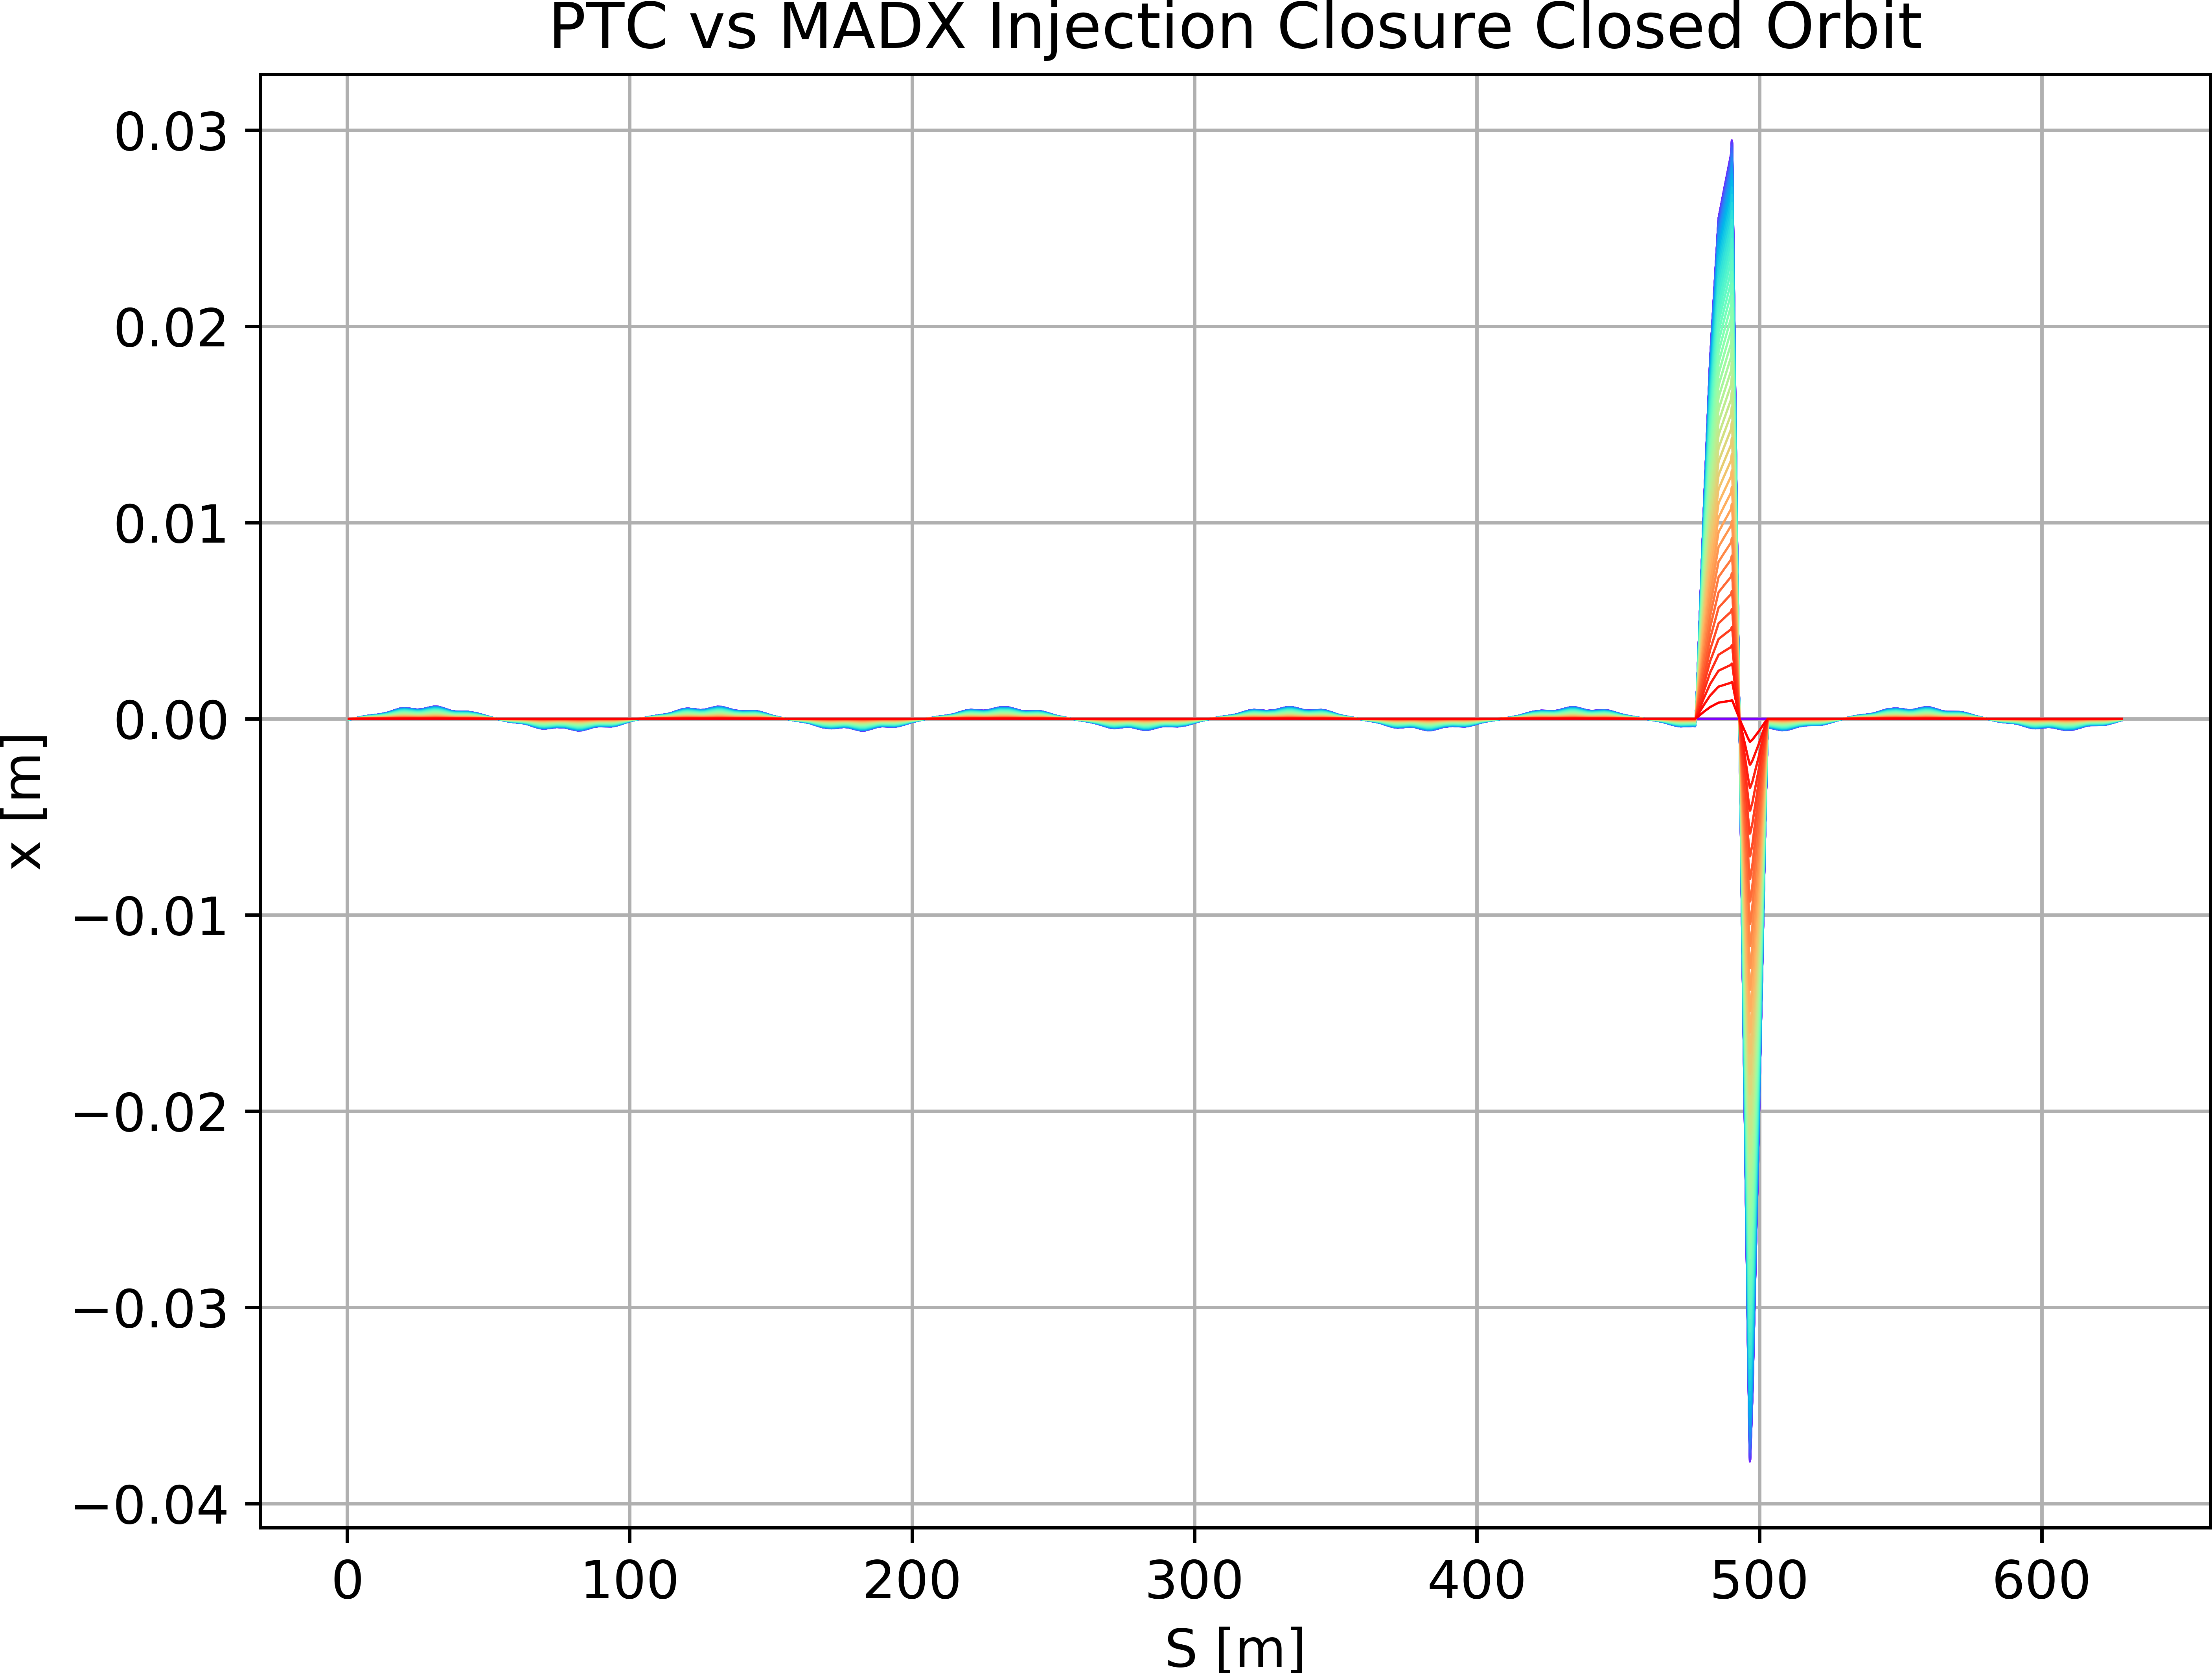
\includegraphics[width=0.45\textwidth]{No_Sext/00_HKICKER/PTC_cf_MADX_Closed_Orbit00_Split_HKICKER_with_MULTIPOLE.png}~~~~~
            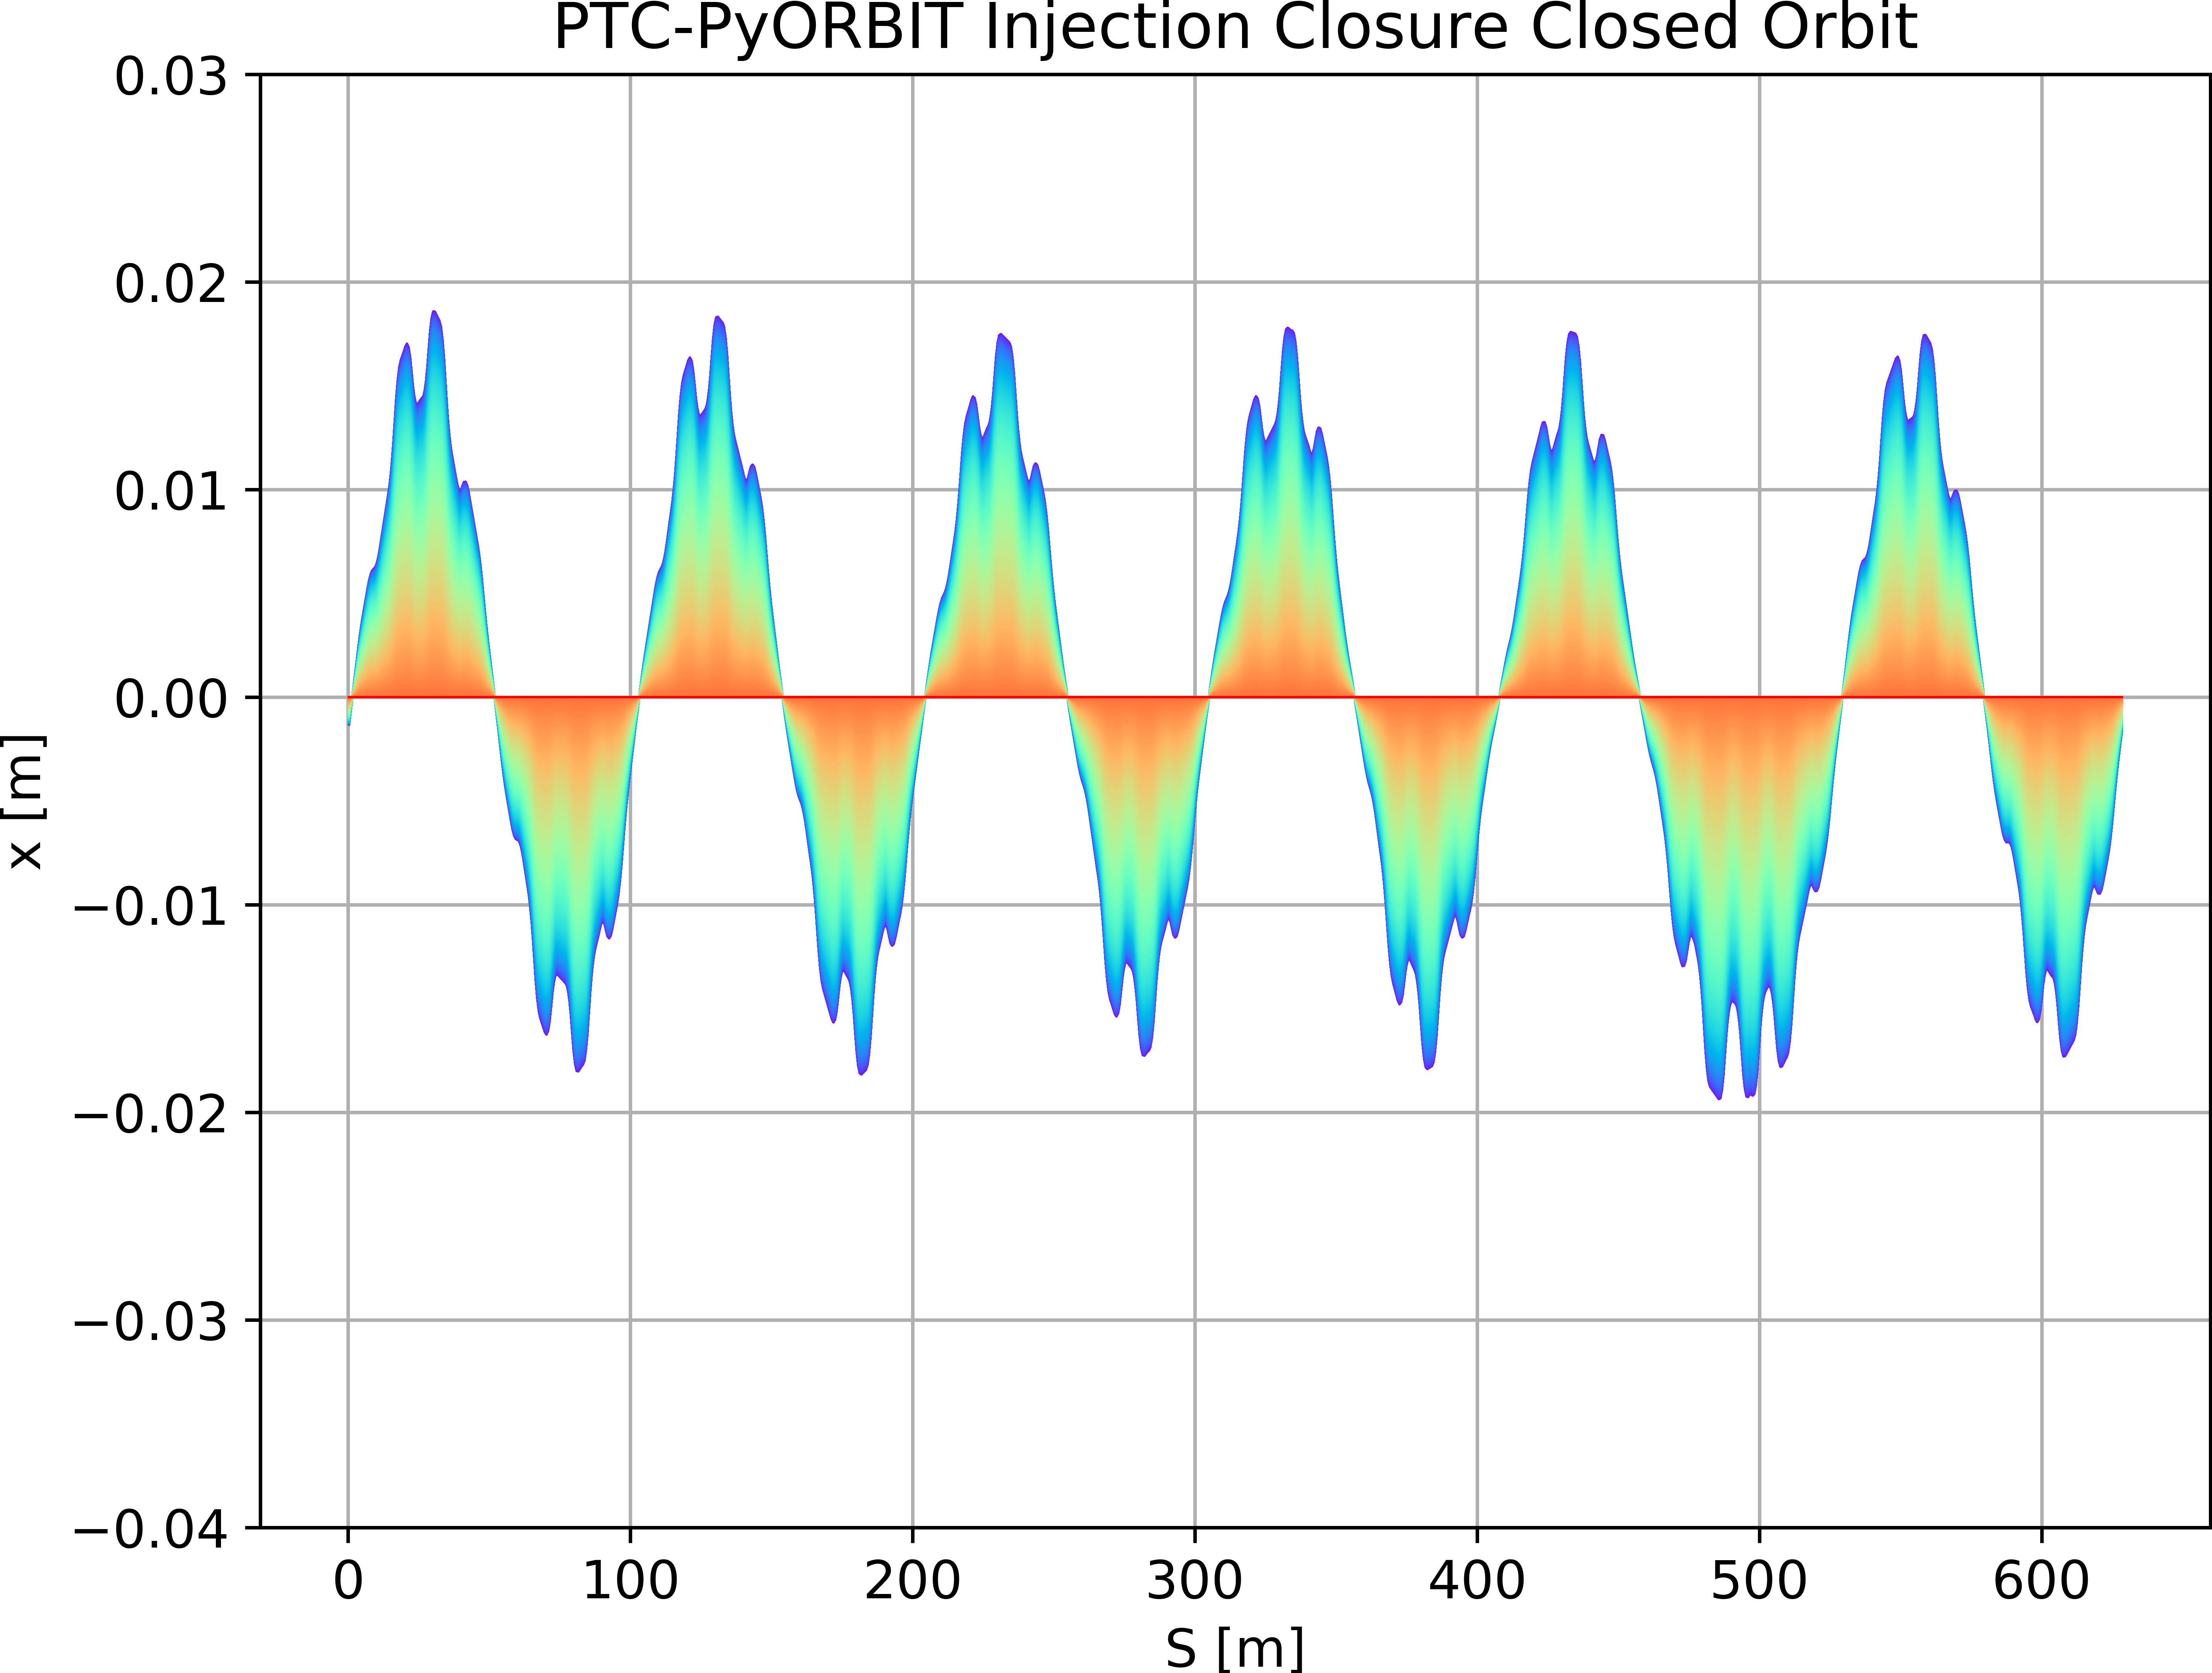
\includegraphics[width=0.45\textwidth]{No_Sext/00_HKICKER/PTC-PyORBIT_Closed_Orbit00_Split_HKICKER_with_MULTIPOLE.png}~~~~~
            \caption{Horizontal closed orbit for split HKICKER + MULTIPOLE: PTC, PyORBIT.}
            \label{fig:00_CO_full}
        \end{figure}
    }
    \frame{
        \frametitle{MULTIPOLE Closed Orbit}
         \begin{figure}
            \centering
            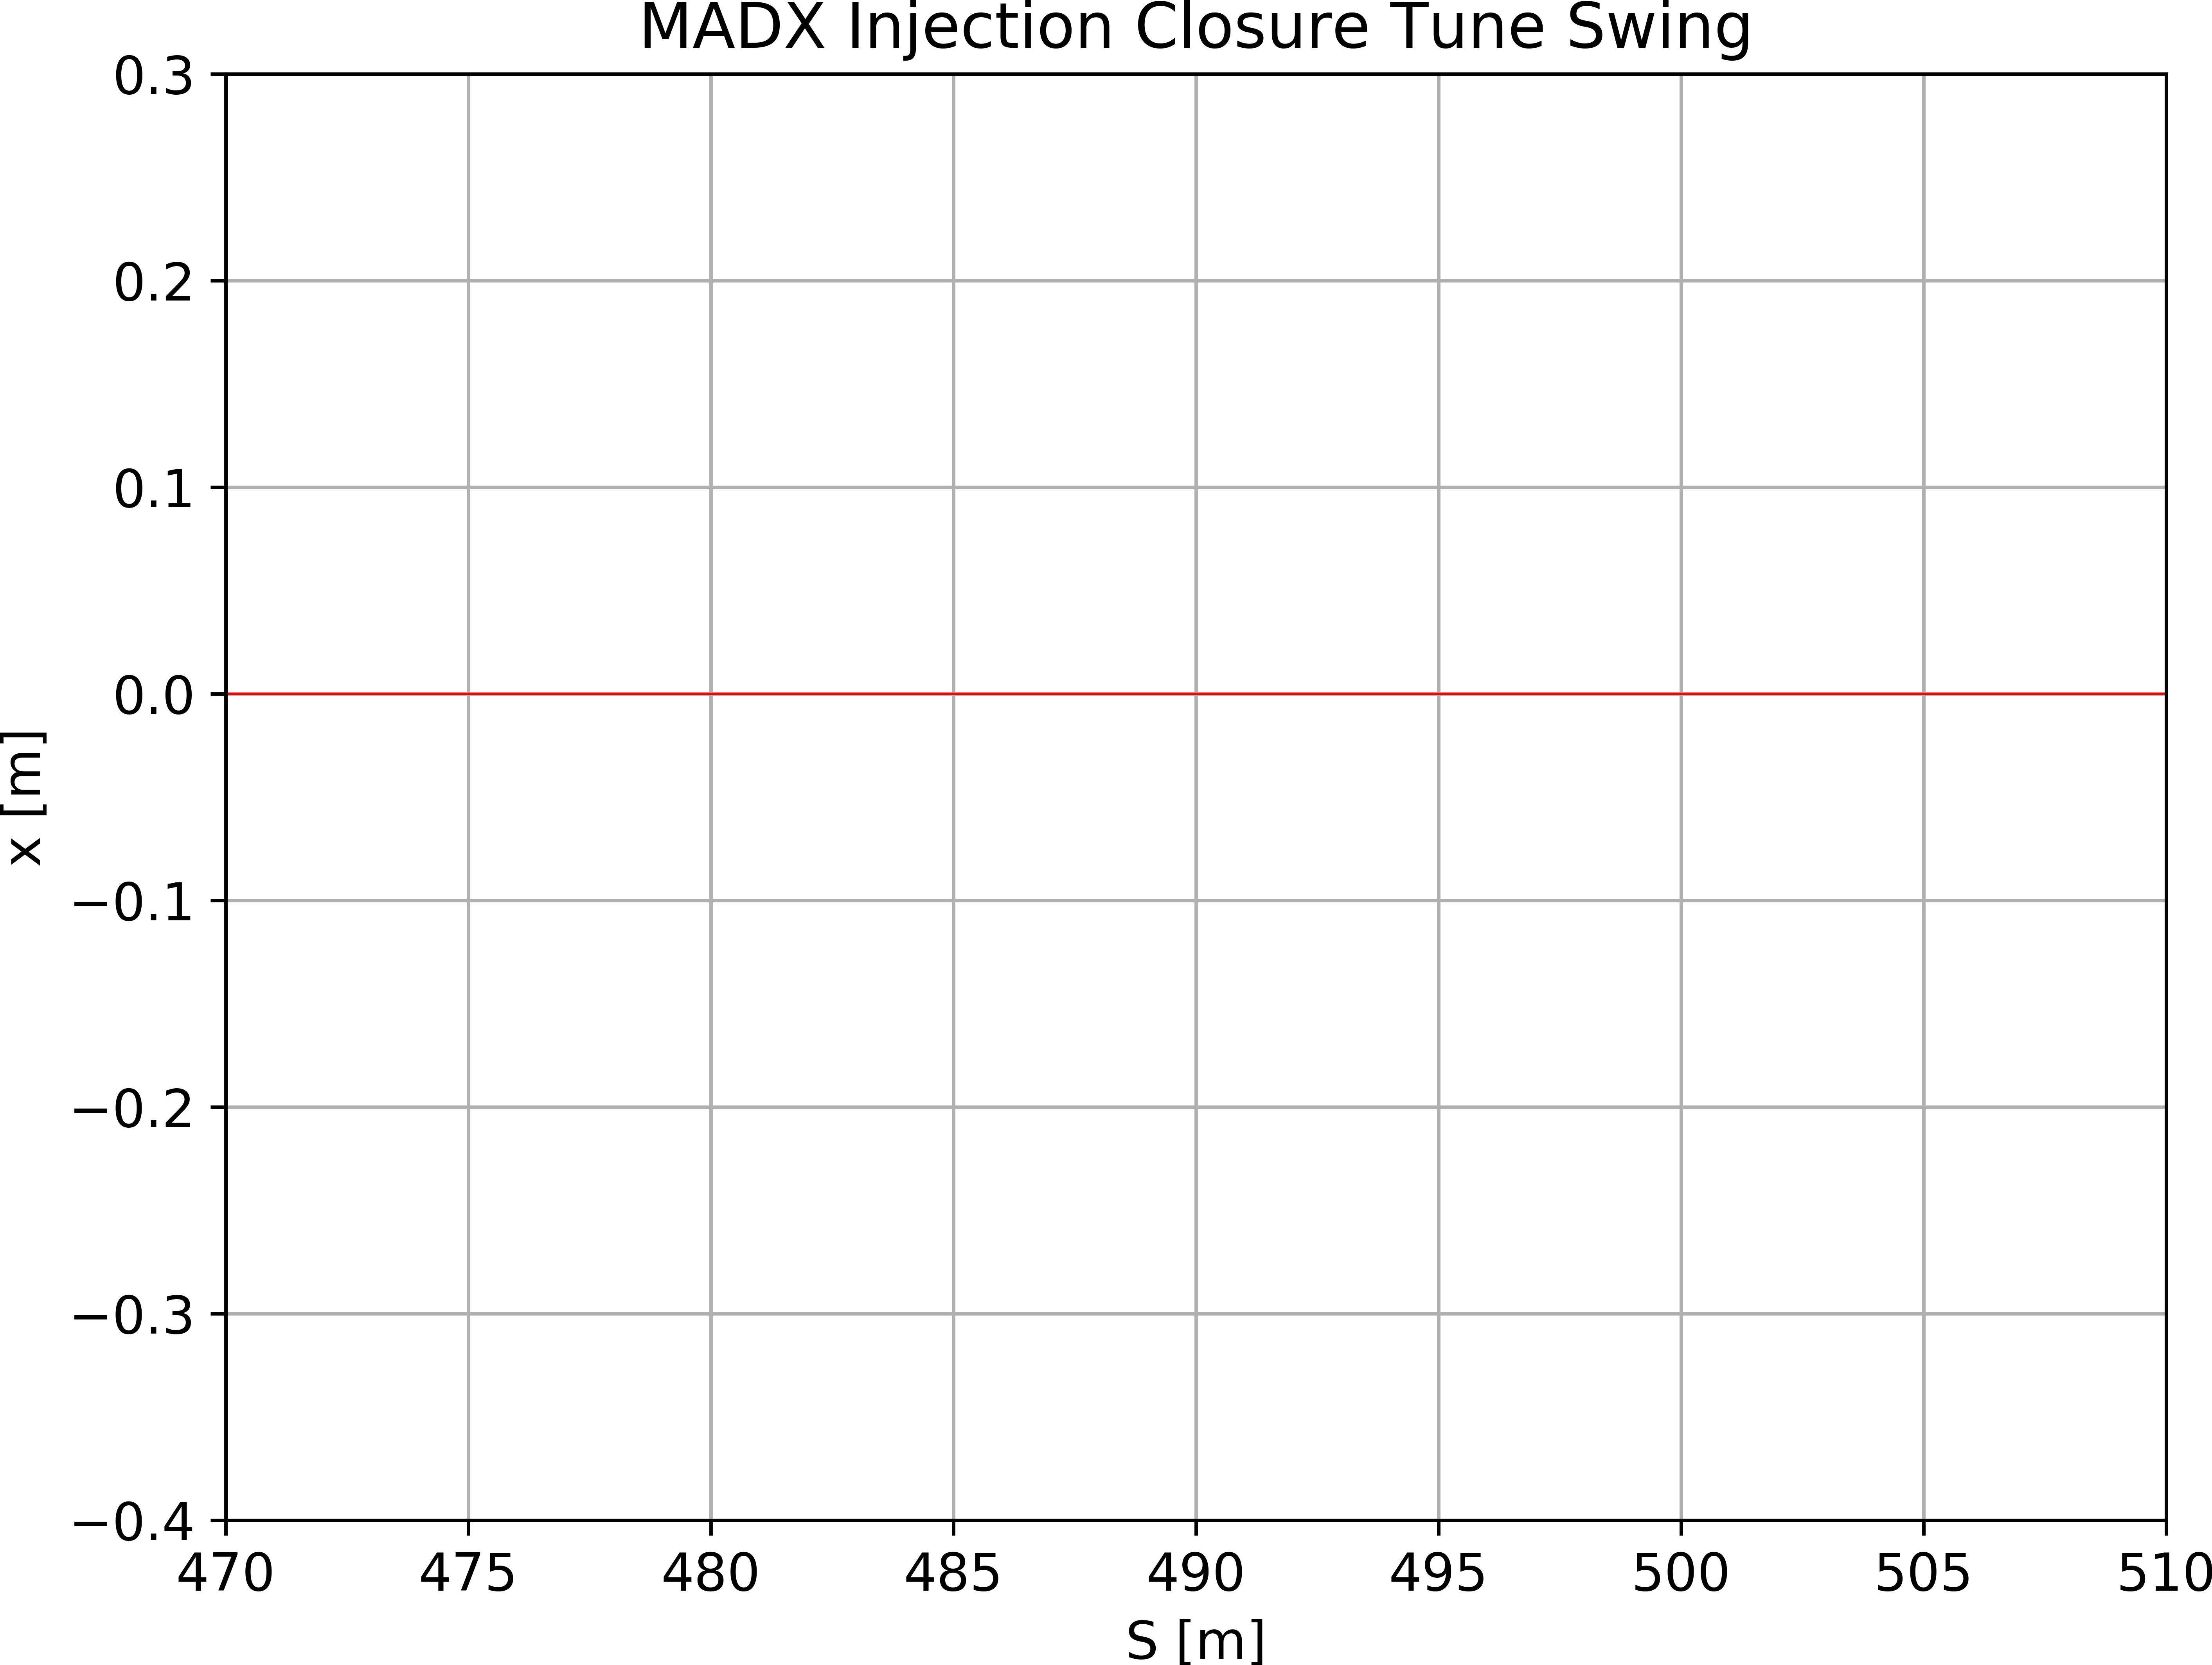
\includegraphics[width=0.3\textwidth]{No_Sext/01_MULTIPOLE/MADX_Closed_Orbit01_MULTIPOLE_zoom.png}~~~~~
            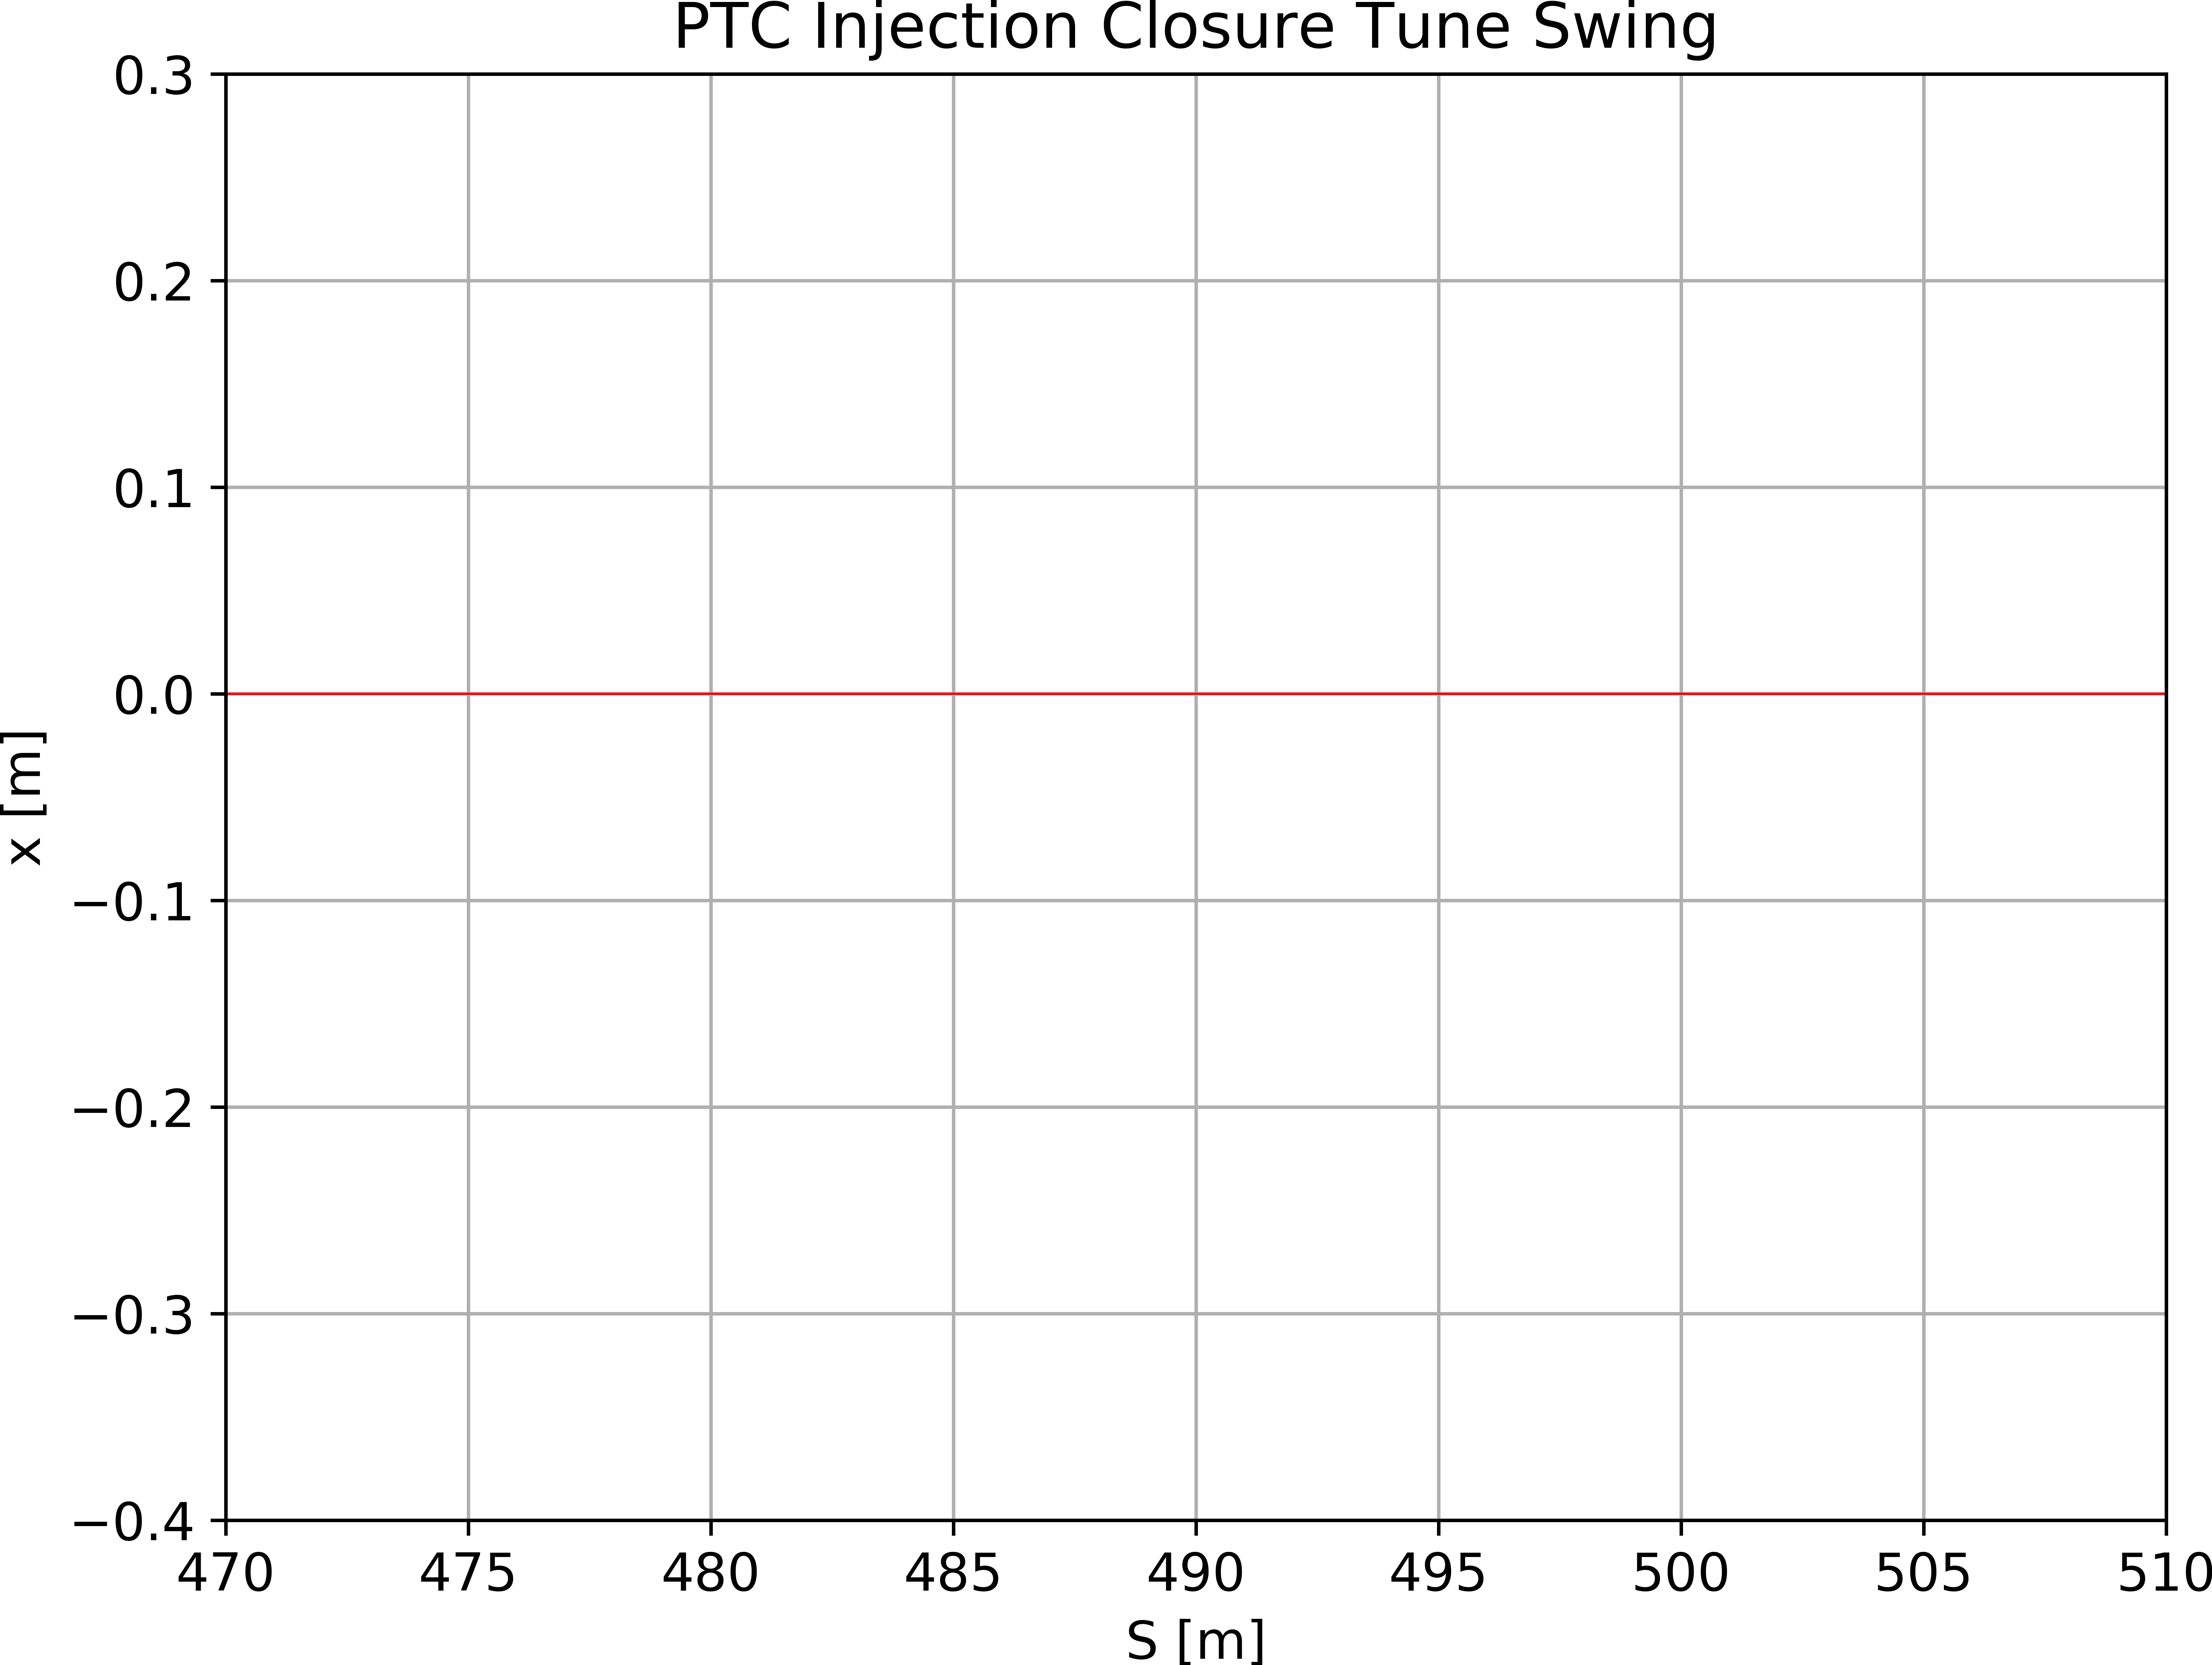
\includegraphics[width=0.3\textwidth]{No_Sext/01_MULTIPOLE/PTC_Closed_Orbit01_MULTIPOLE_zoom.png}~~~~~
            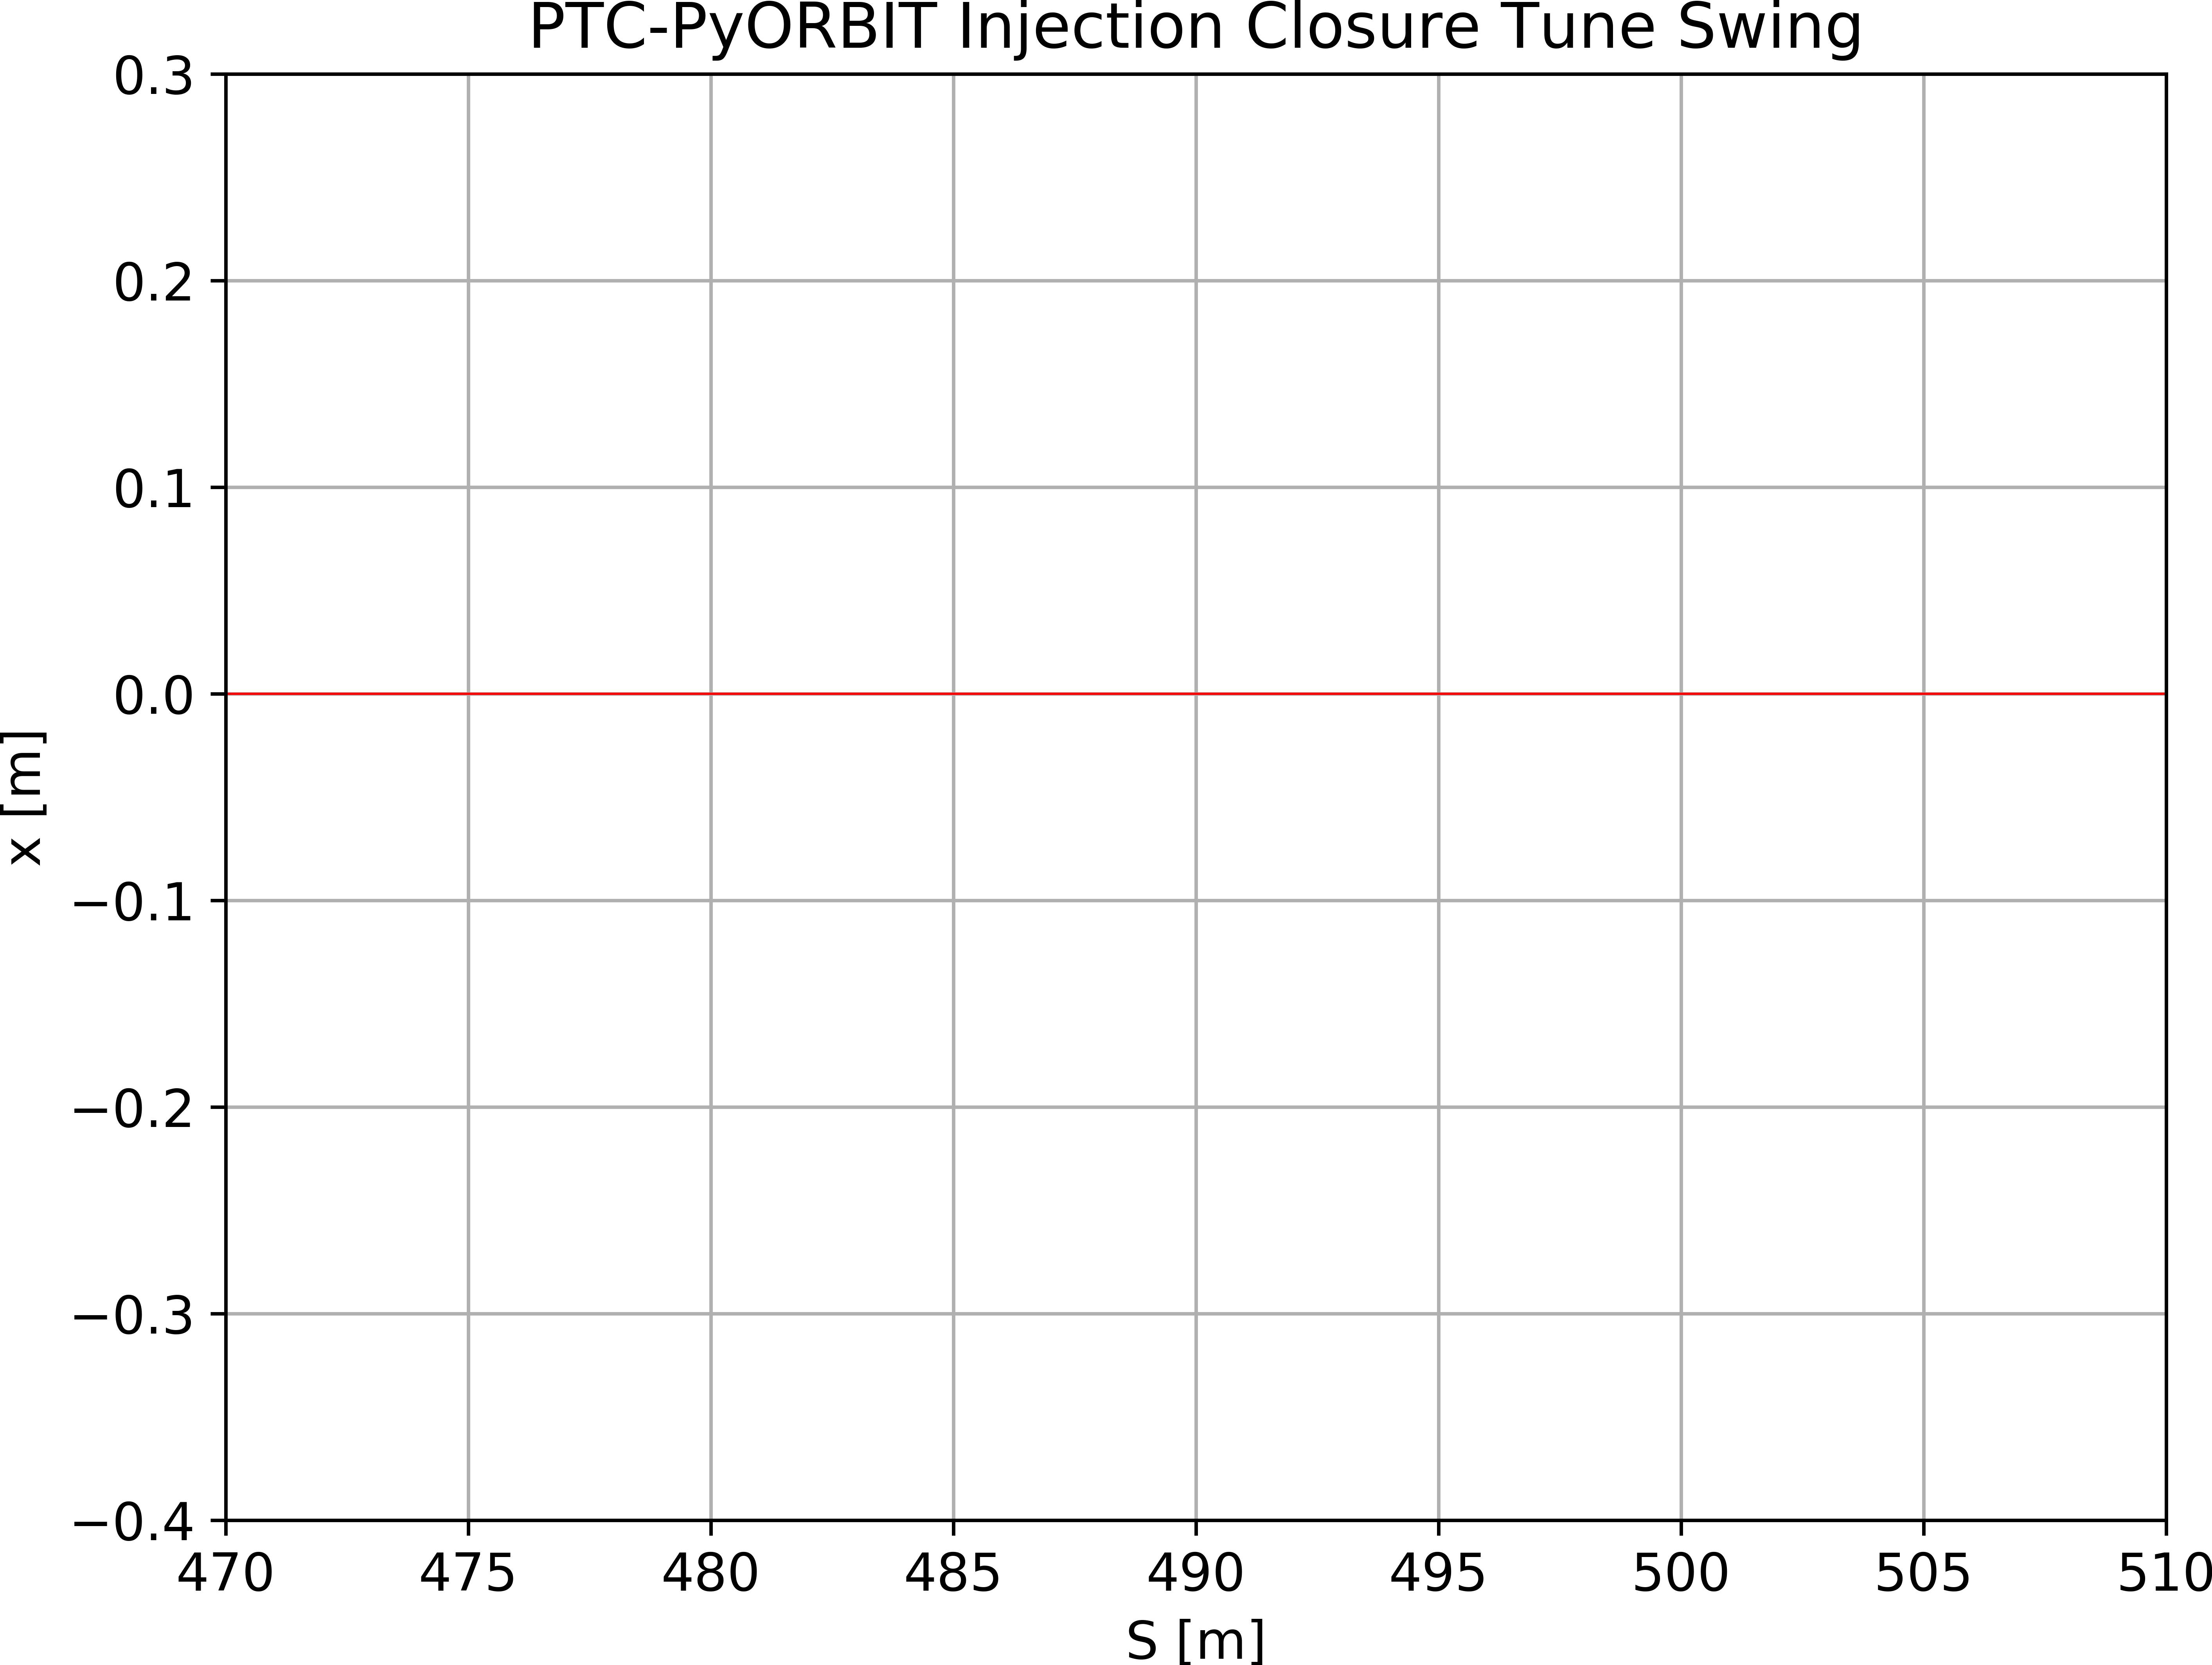
\includegraphics[width=0.3\textwidth]{No_Sext/01_MULTIPOLE/PTC-PyORBIT_Closed_Orbit01_MULTIPOLE_zoom.png}
            \caption{Horizontal closed orbit for MULTIPOLE: MAD-X, PTC, PyORBIT.}
            \label{fig:01_CO_zoom}
        \end{figure}
    }
    \frame{
        \frametitle{QUADRUPOLE (as errors) Closed Orbit}
         \begin{figure}
            \centering
            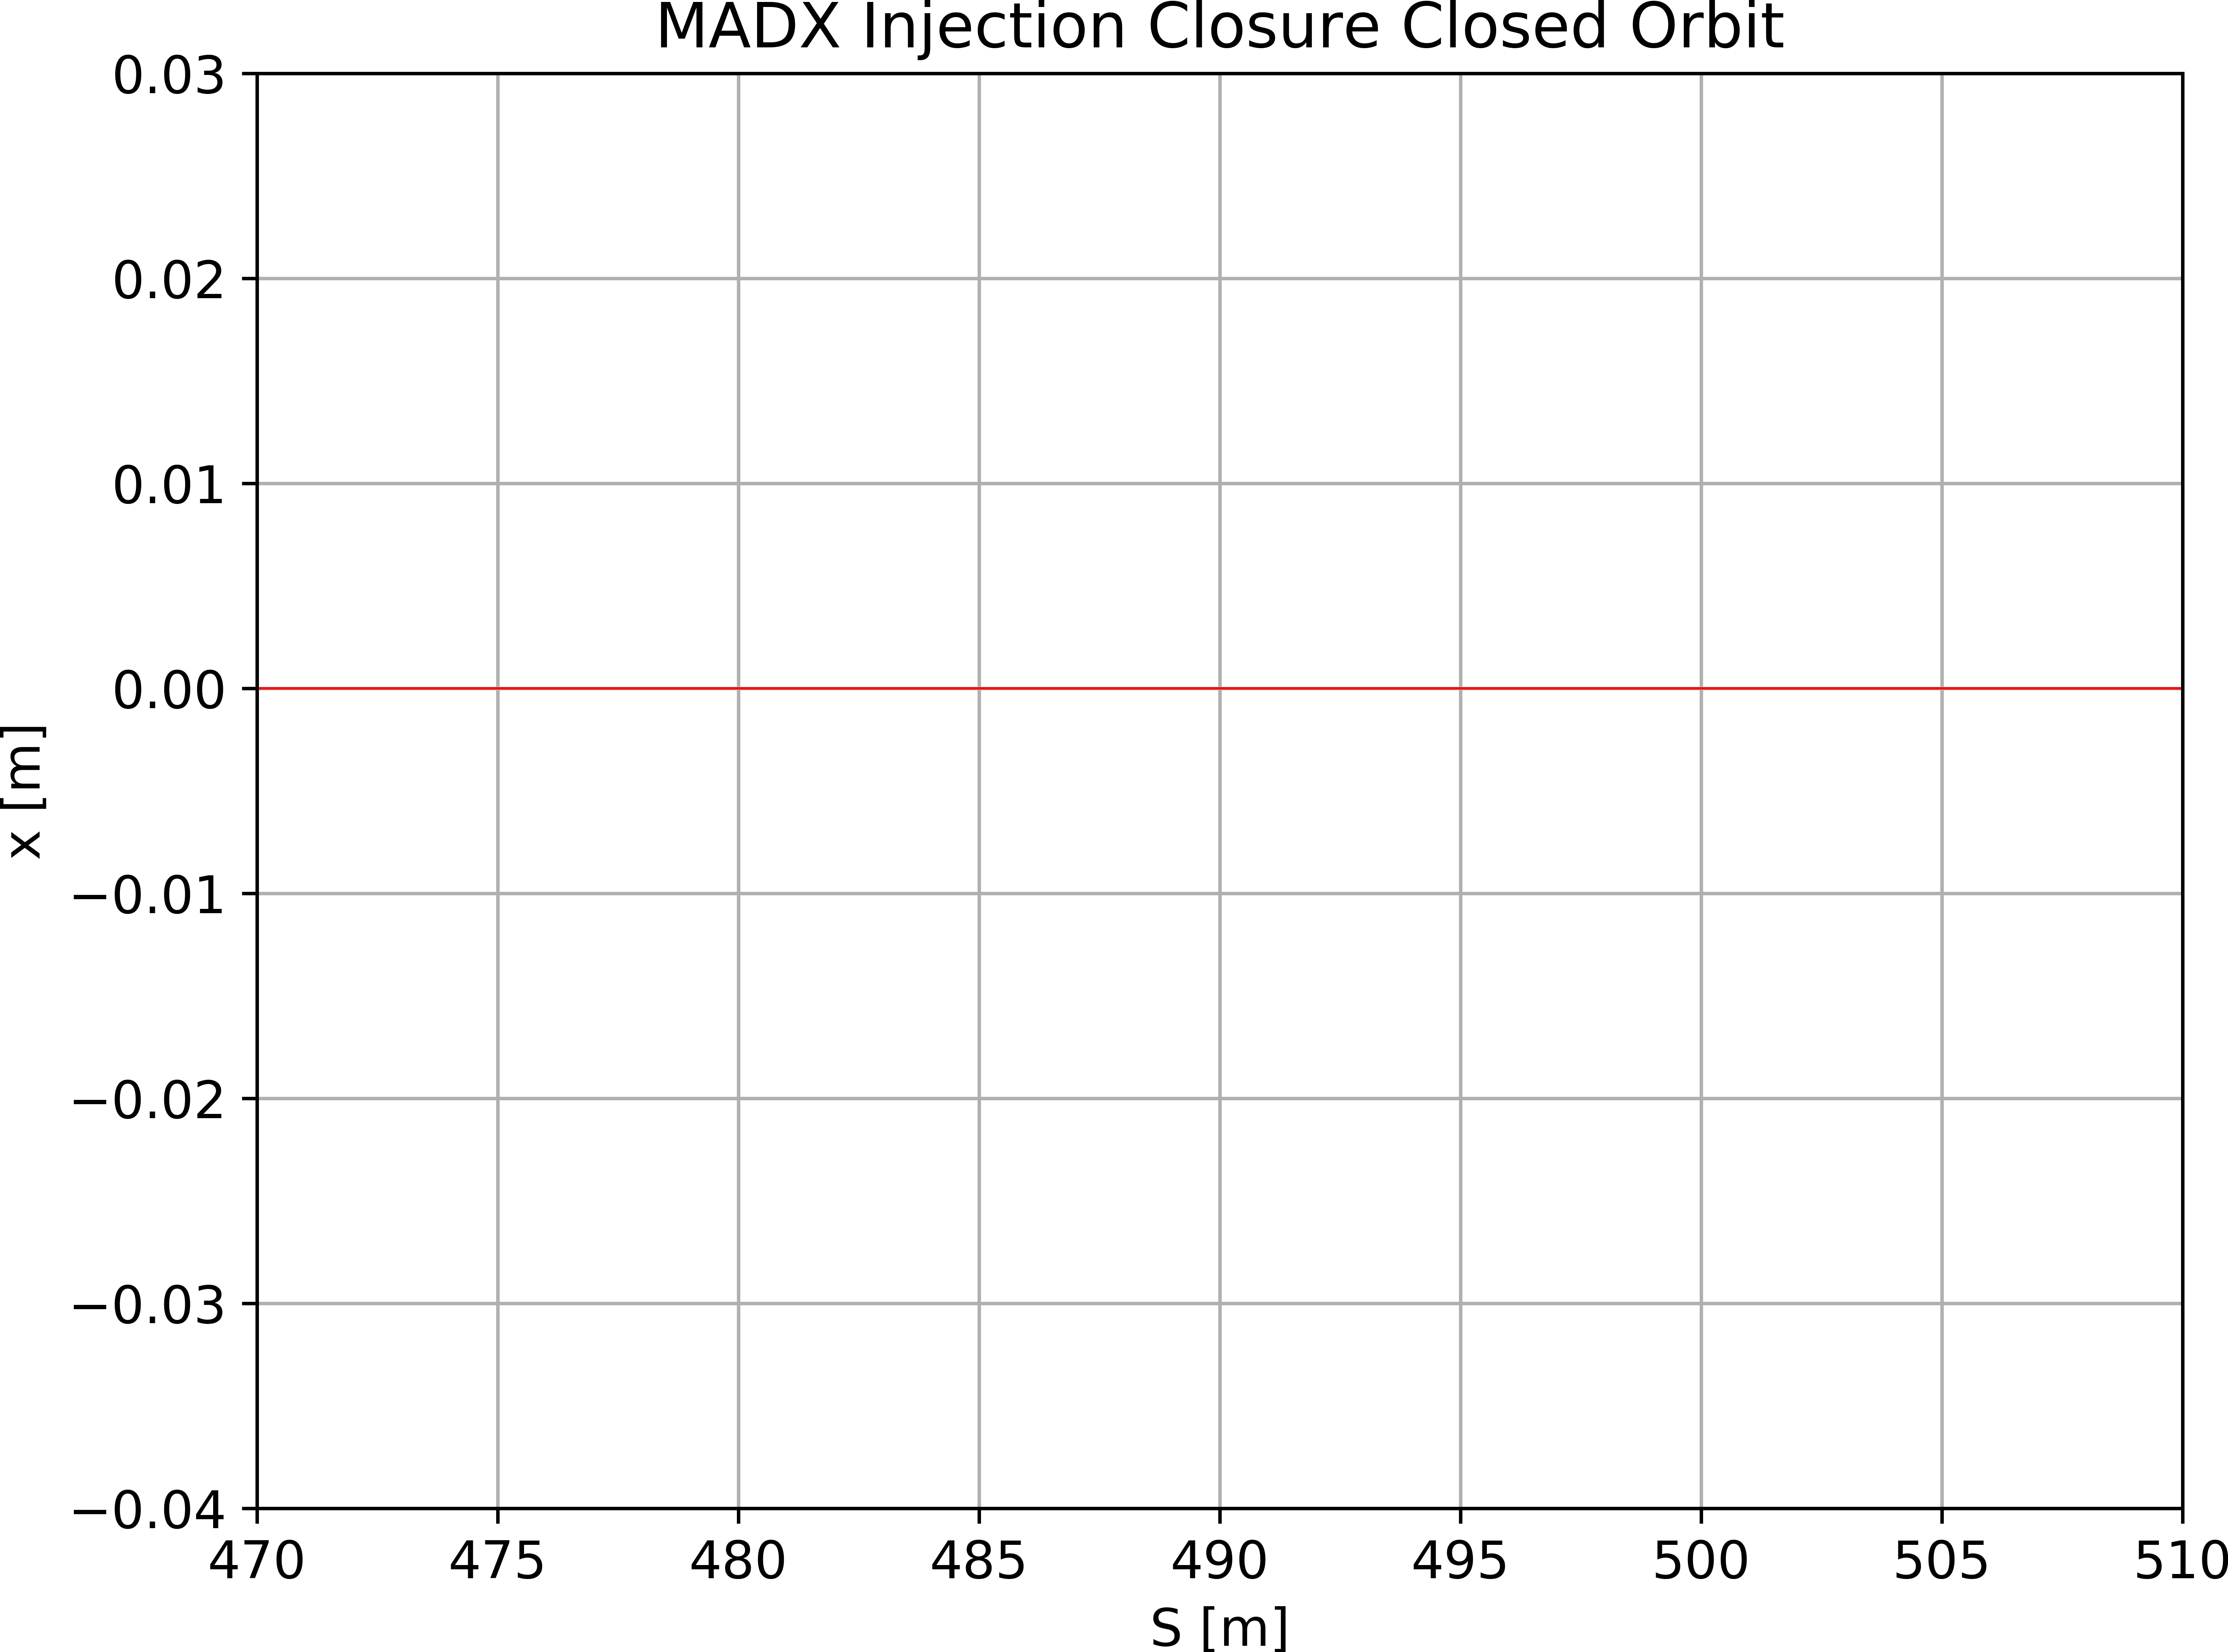
\includegraphics[width=0.3\textwidth]{No_Sext/02_QUADRUPOLE/MADX_Closed_Orbit02_QUADRUPOLE_zoom.png}~~~~~
            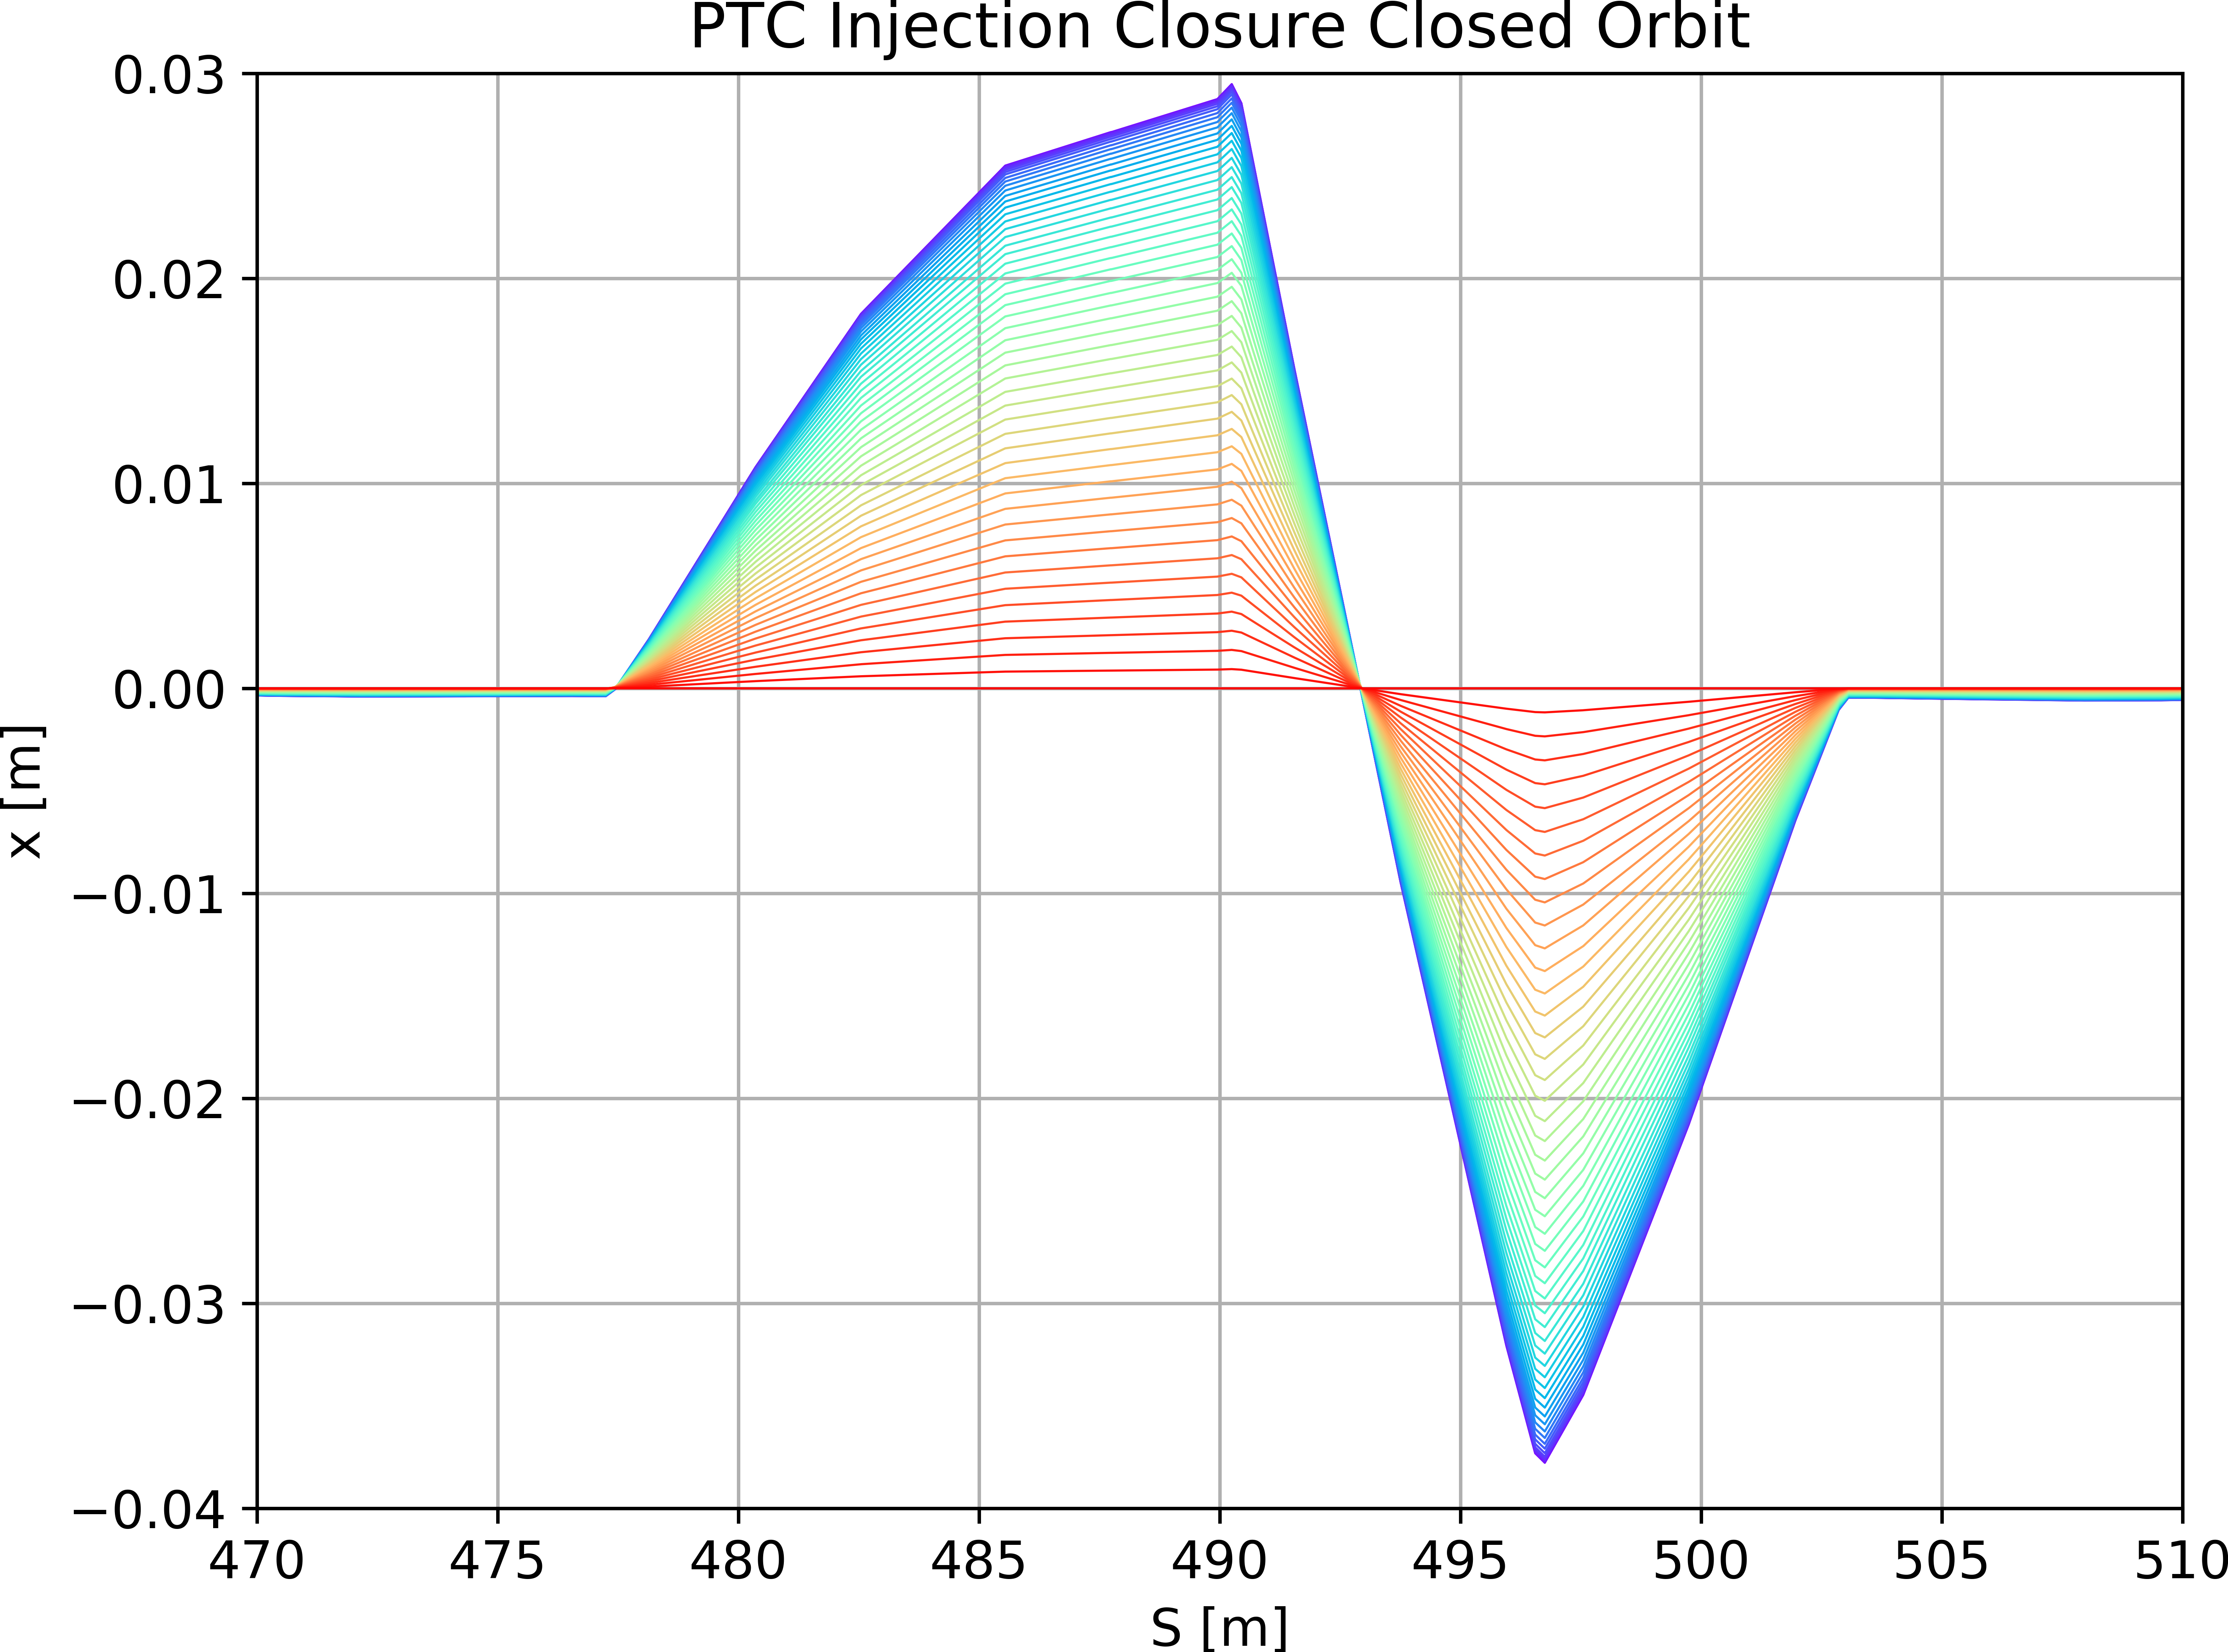
\includegraphics[width=0.3\textwidth]{No_Sext/02_QUADRUPOLE/PTC_Closed_Orbit02_QUADRUPOLE_zoom.png}~~~~~
            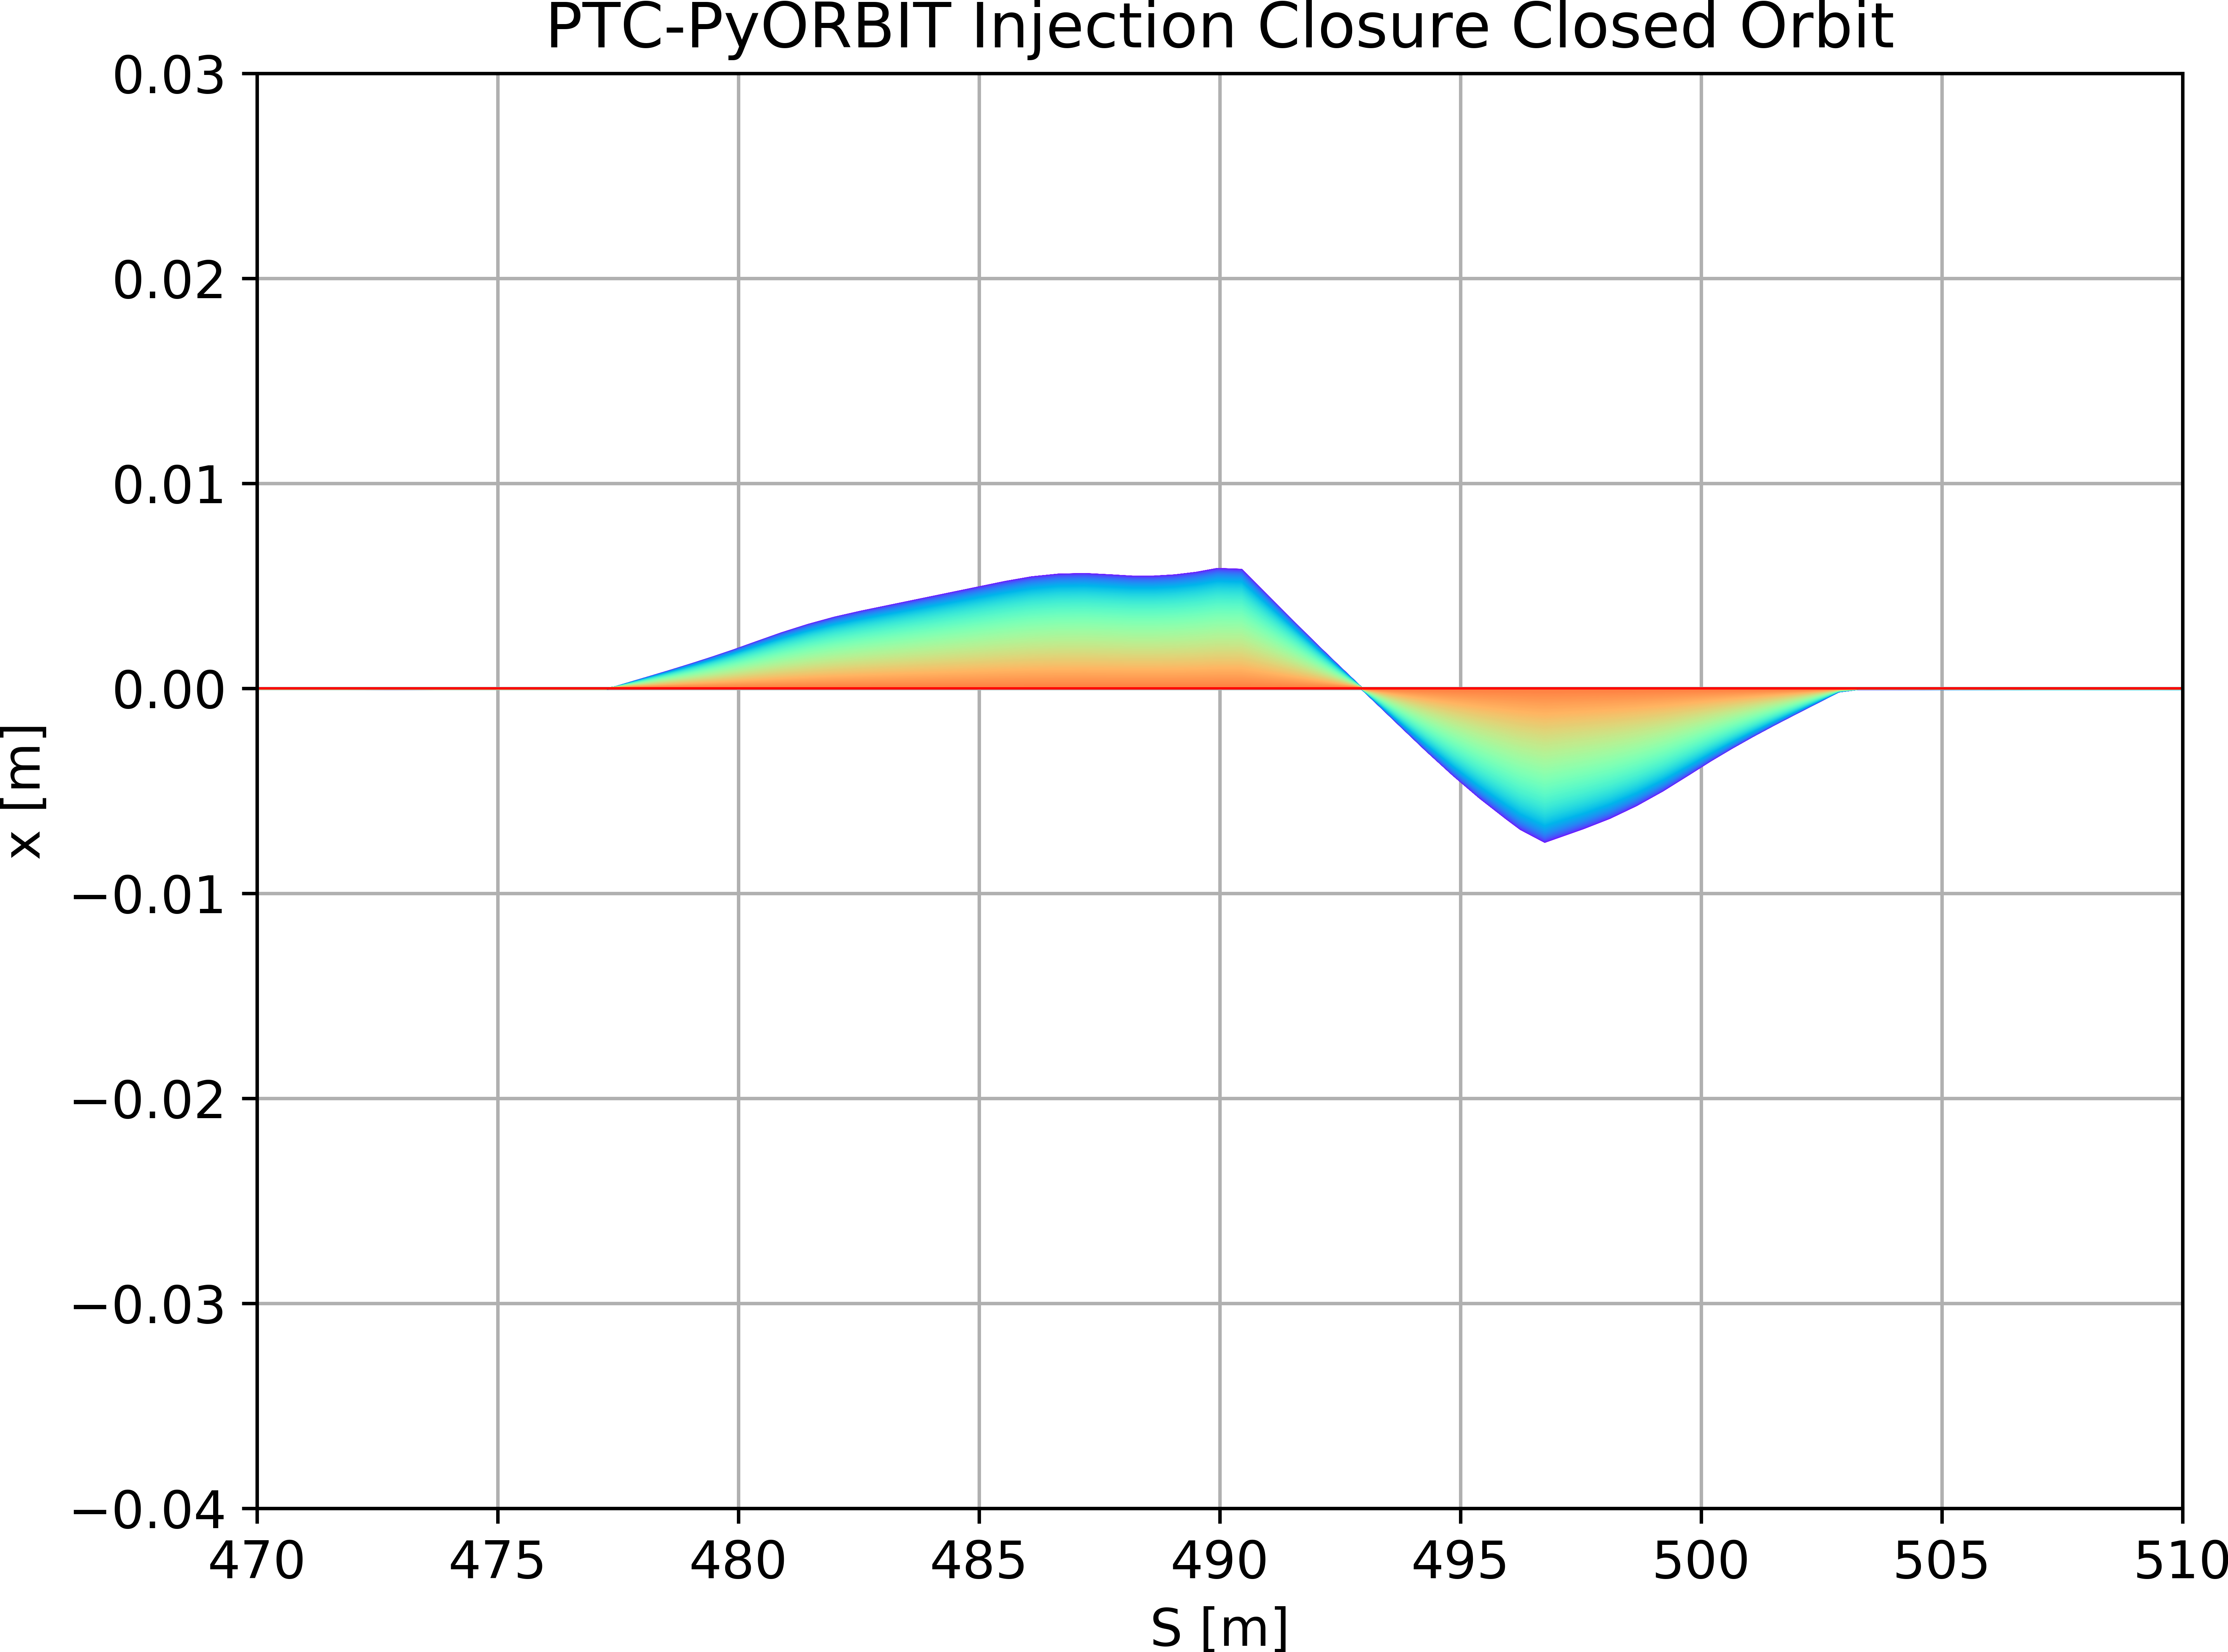
\includegraphics[width=0.3\textwidth]{No_Sext/02_QUADRUPOLE/PTC-PyORBIT_Closed_Orbit02_QUADRUPOLE_zoom.png}
            \caption{Horizontal closed orbit for QUADRUPOLE: MAD-X, PTC, PyORBIT.}
            \label{fig:02_CO_zoom}
        \end{figure}
    }
    \frame{
        \frametitle{SBEND (as errors) Closed Orbit}
         \begin{figure}
            \centering
            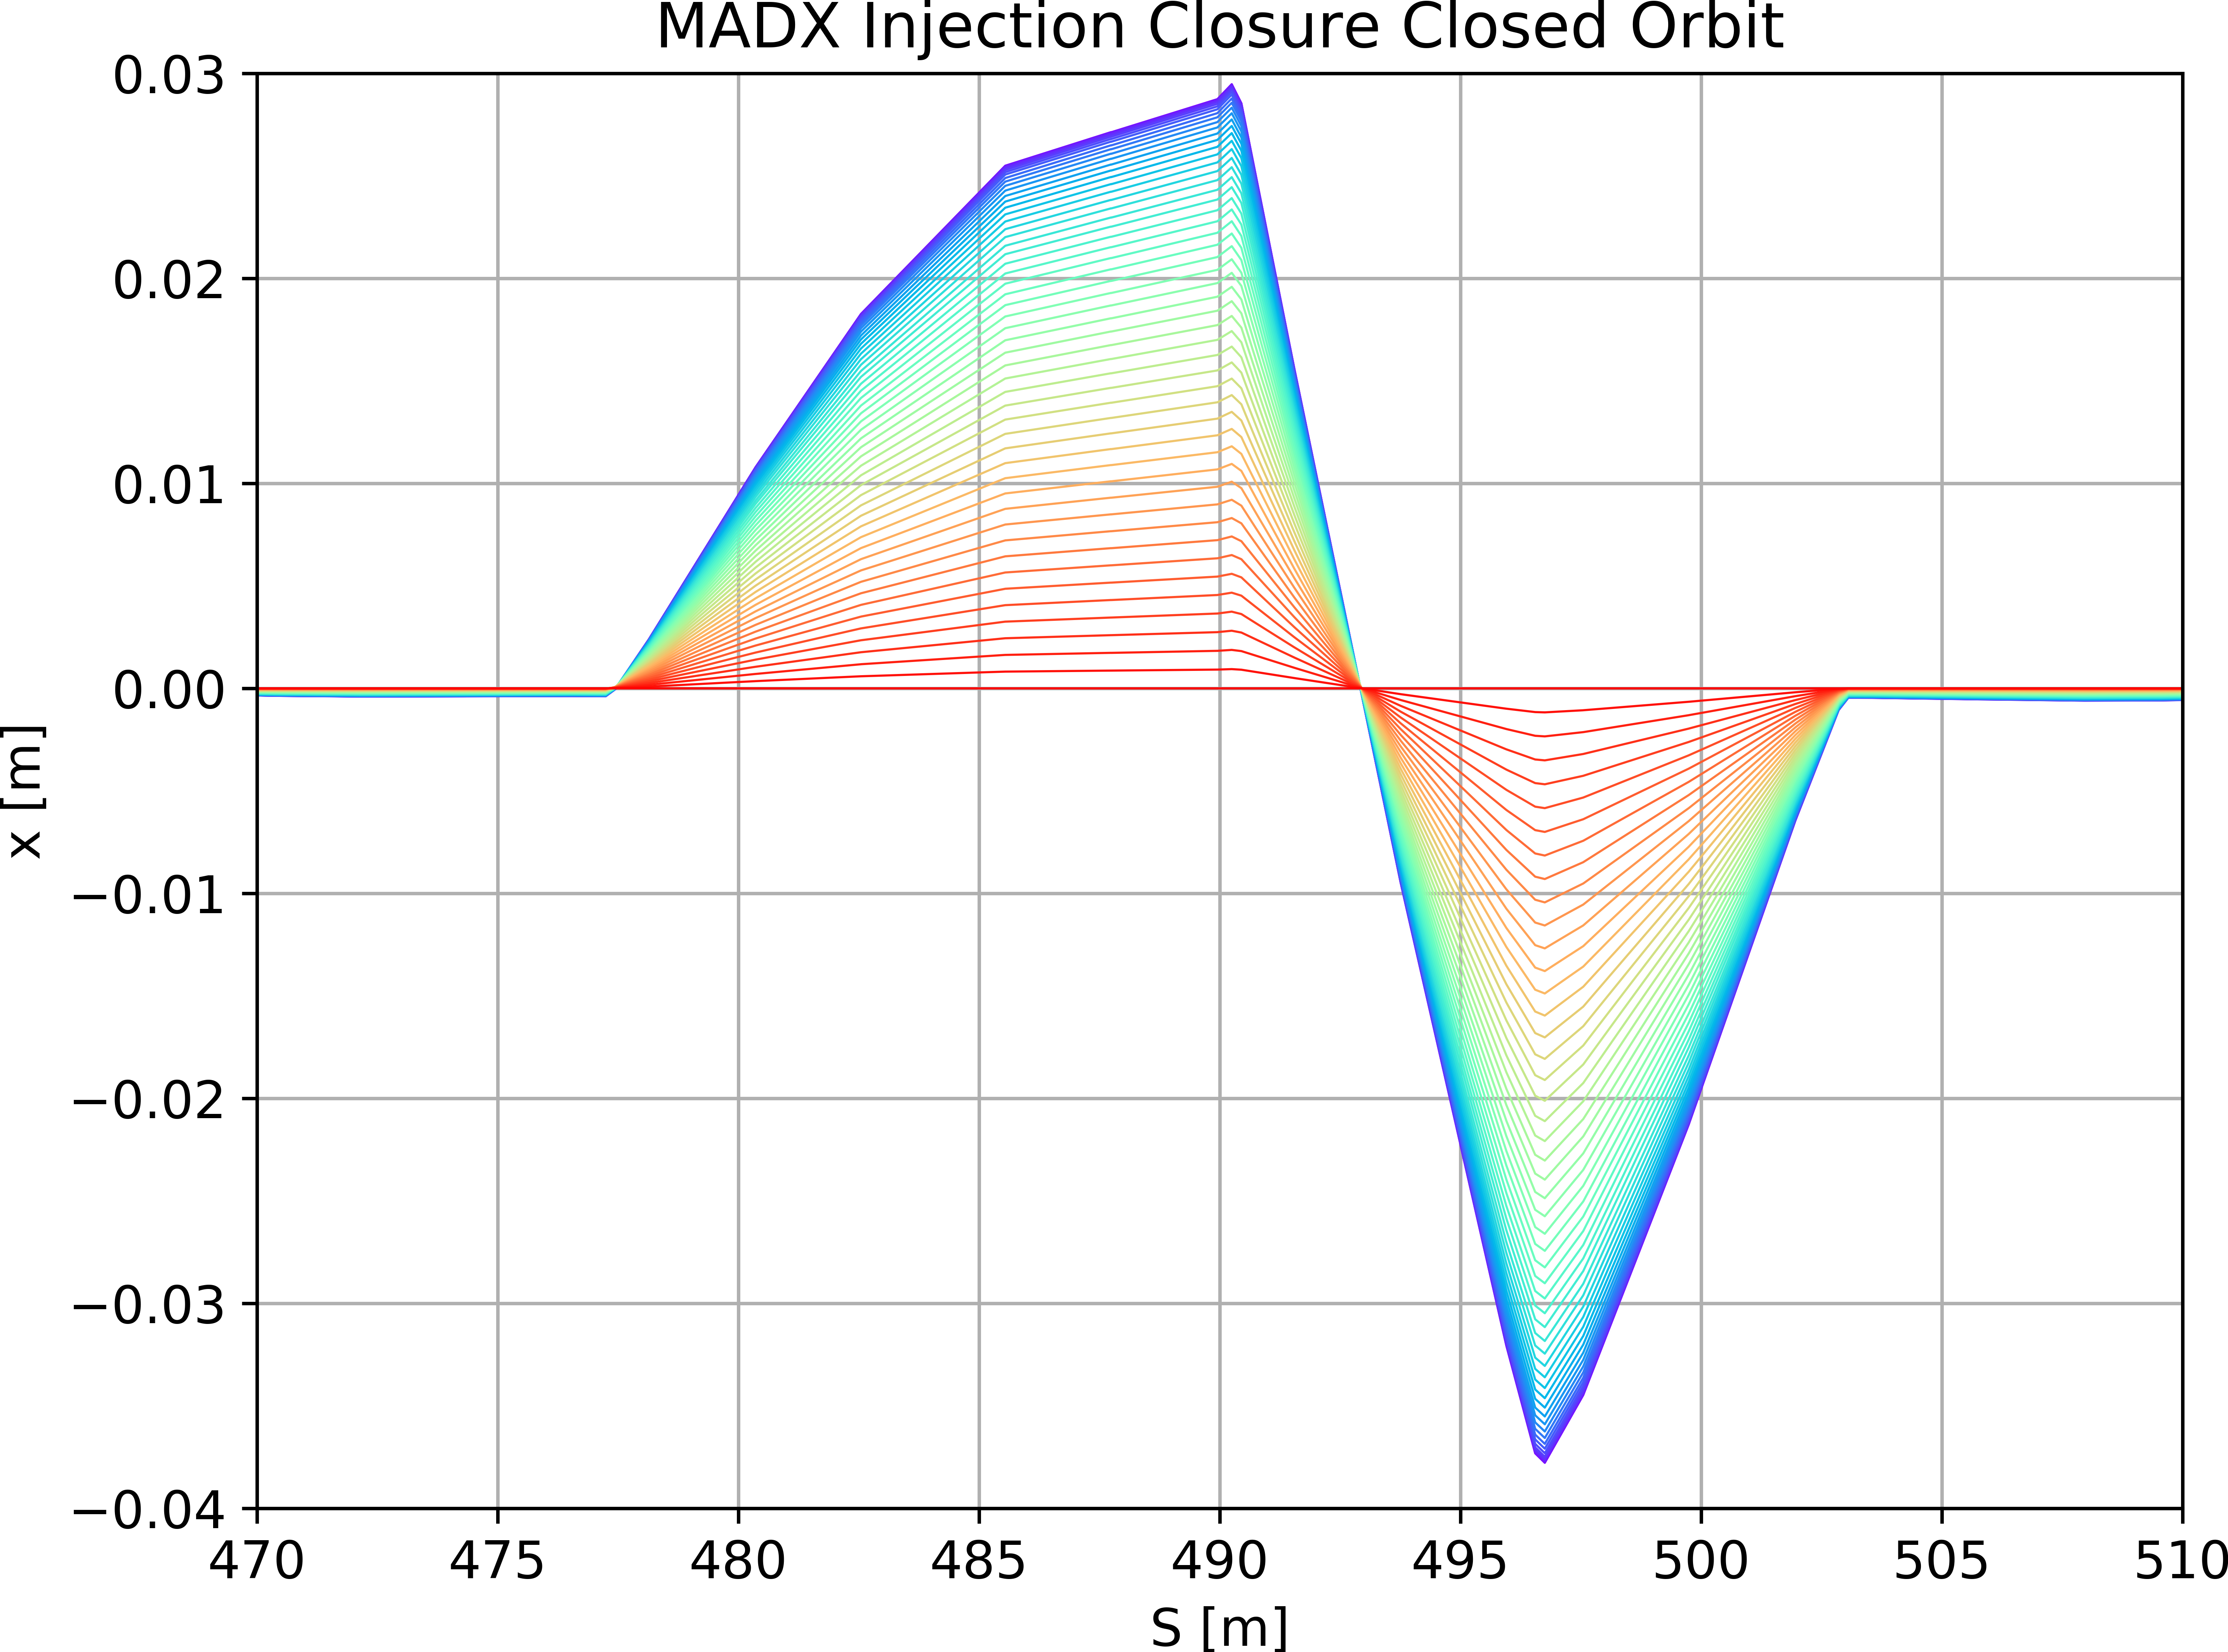
\includegraphics[width=0.3\textwidth]{No_Sext/03_SBEND/MADX_Closed_Orbit03_SBEND_zoom.png}~~~~~
            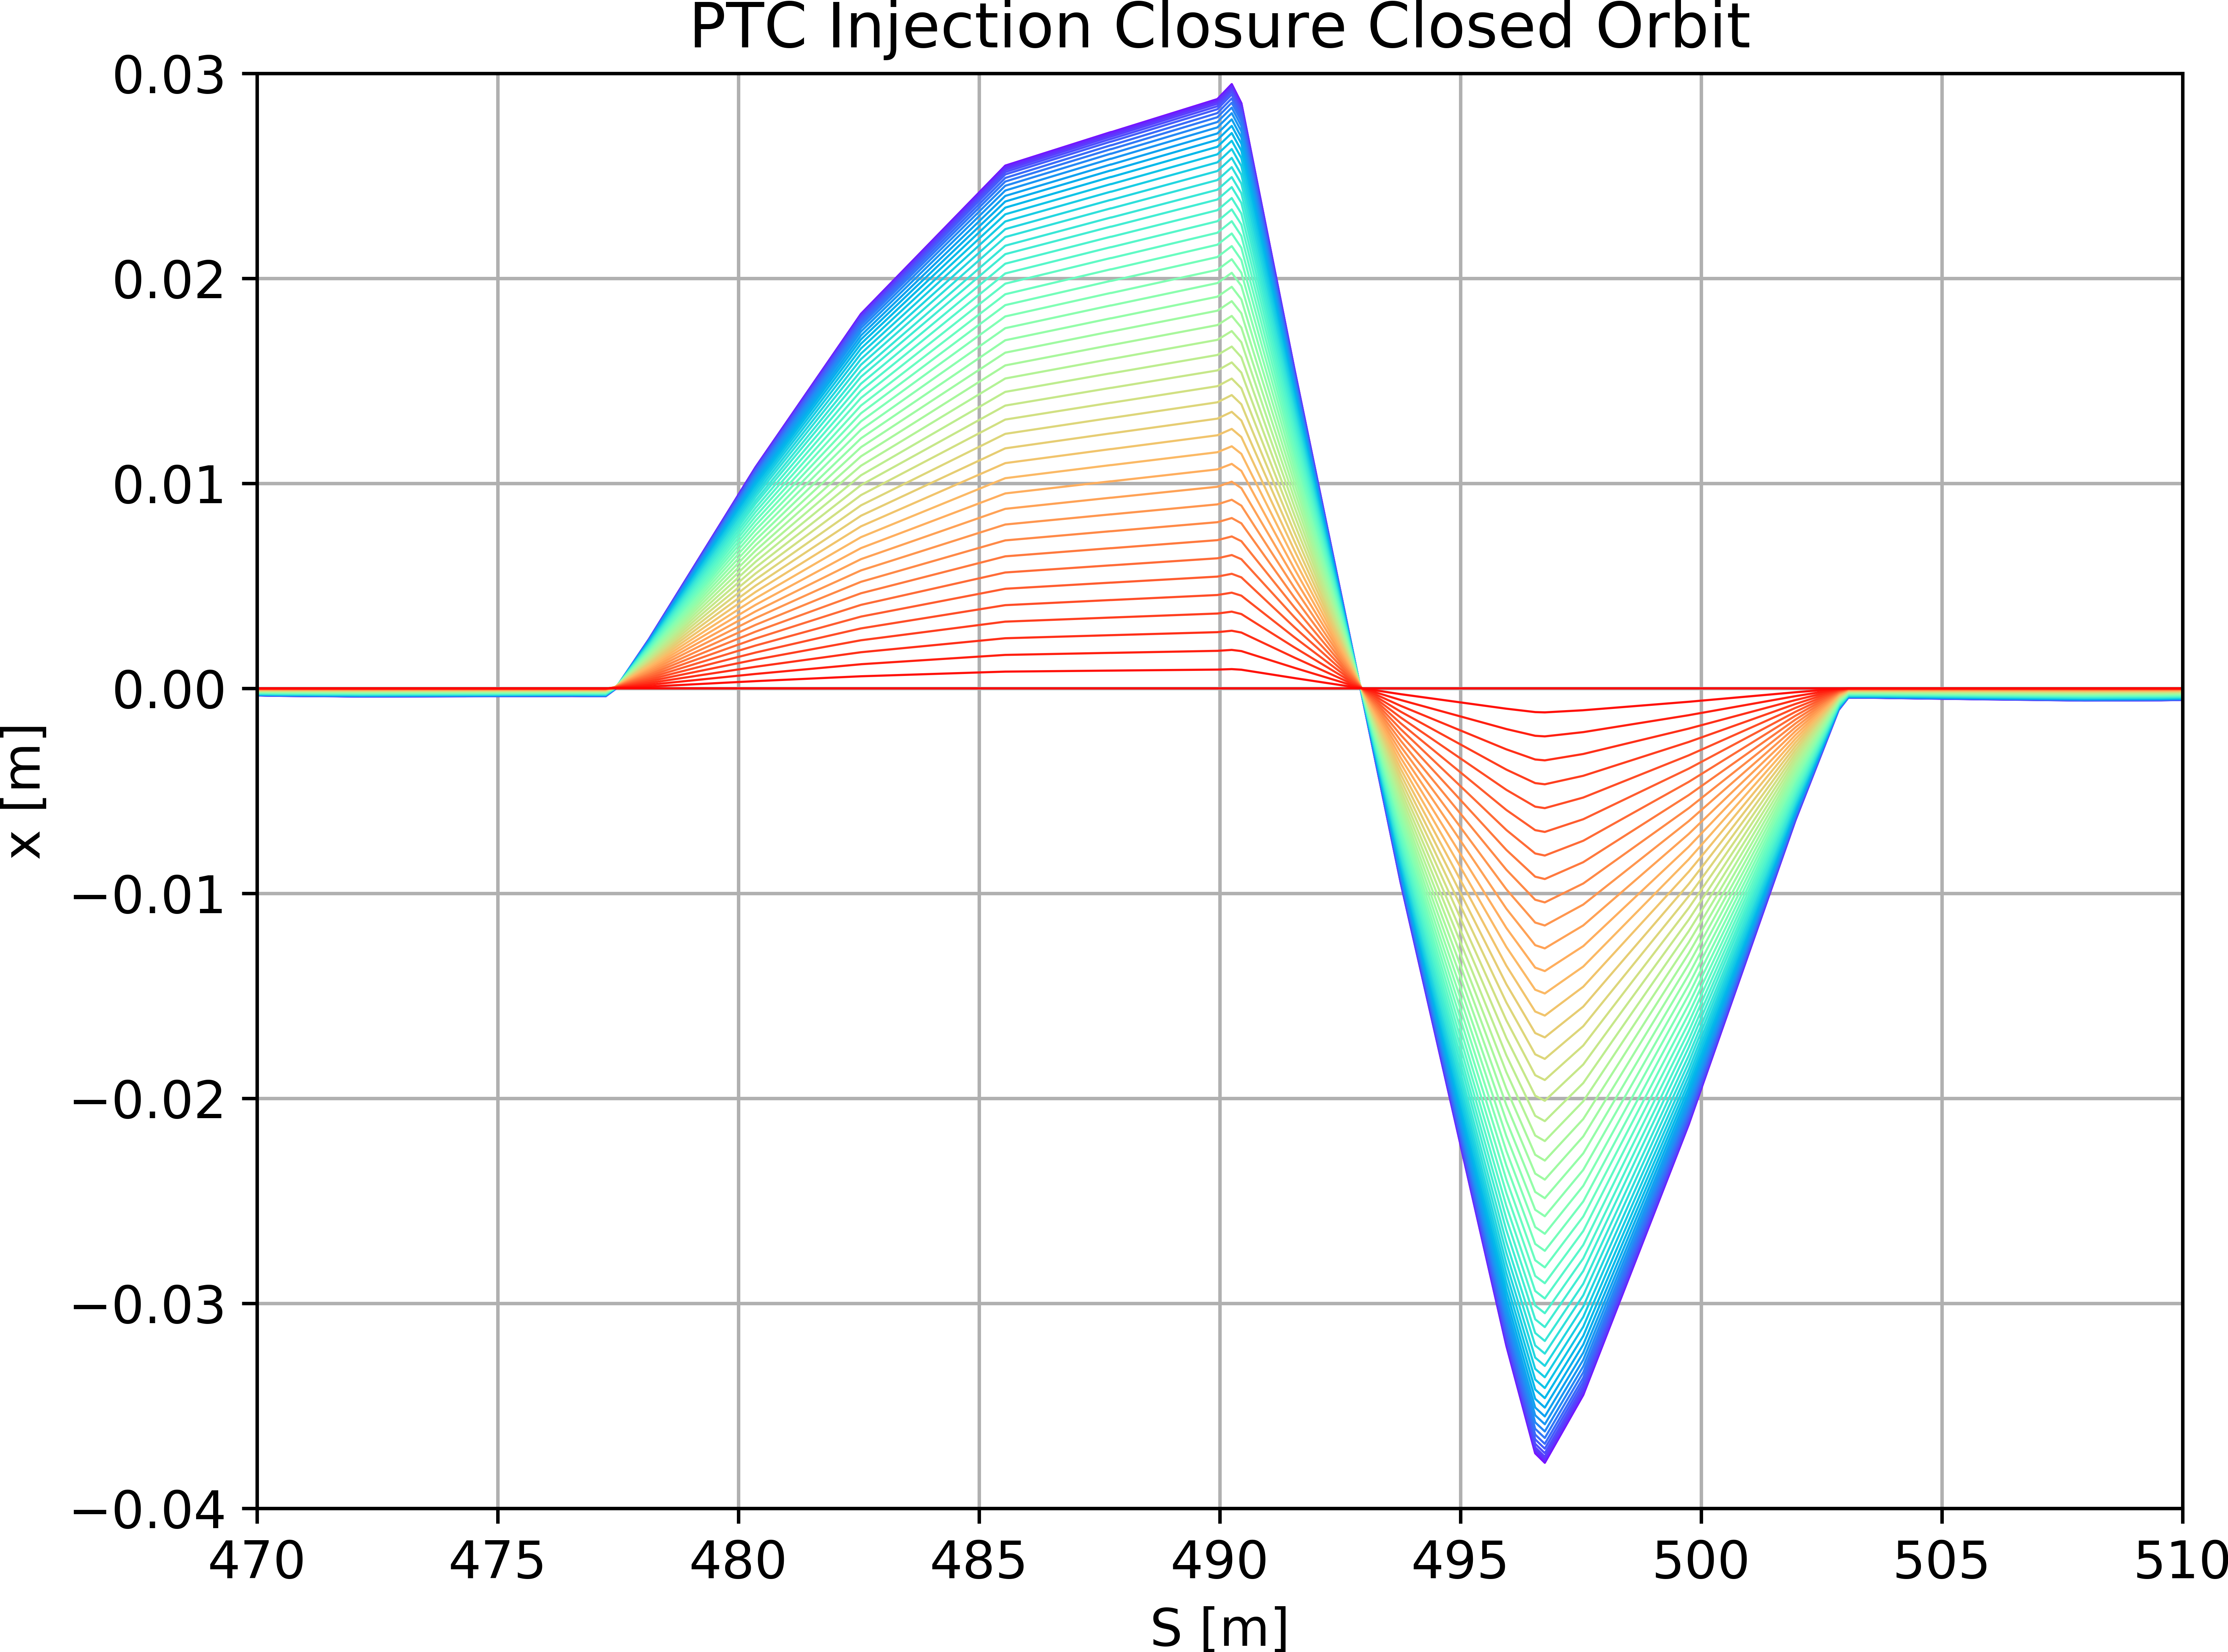
\includegraphics[width=0.3\textwidth]{No_Sext/03_SBEND/PTC_Closed_Orbit03_SBEND_zoom.png}~~~~~
            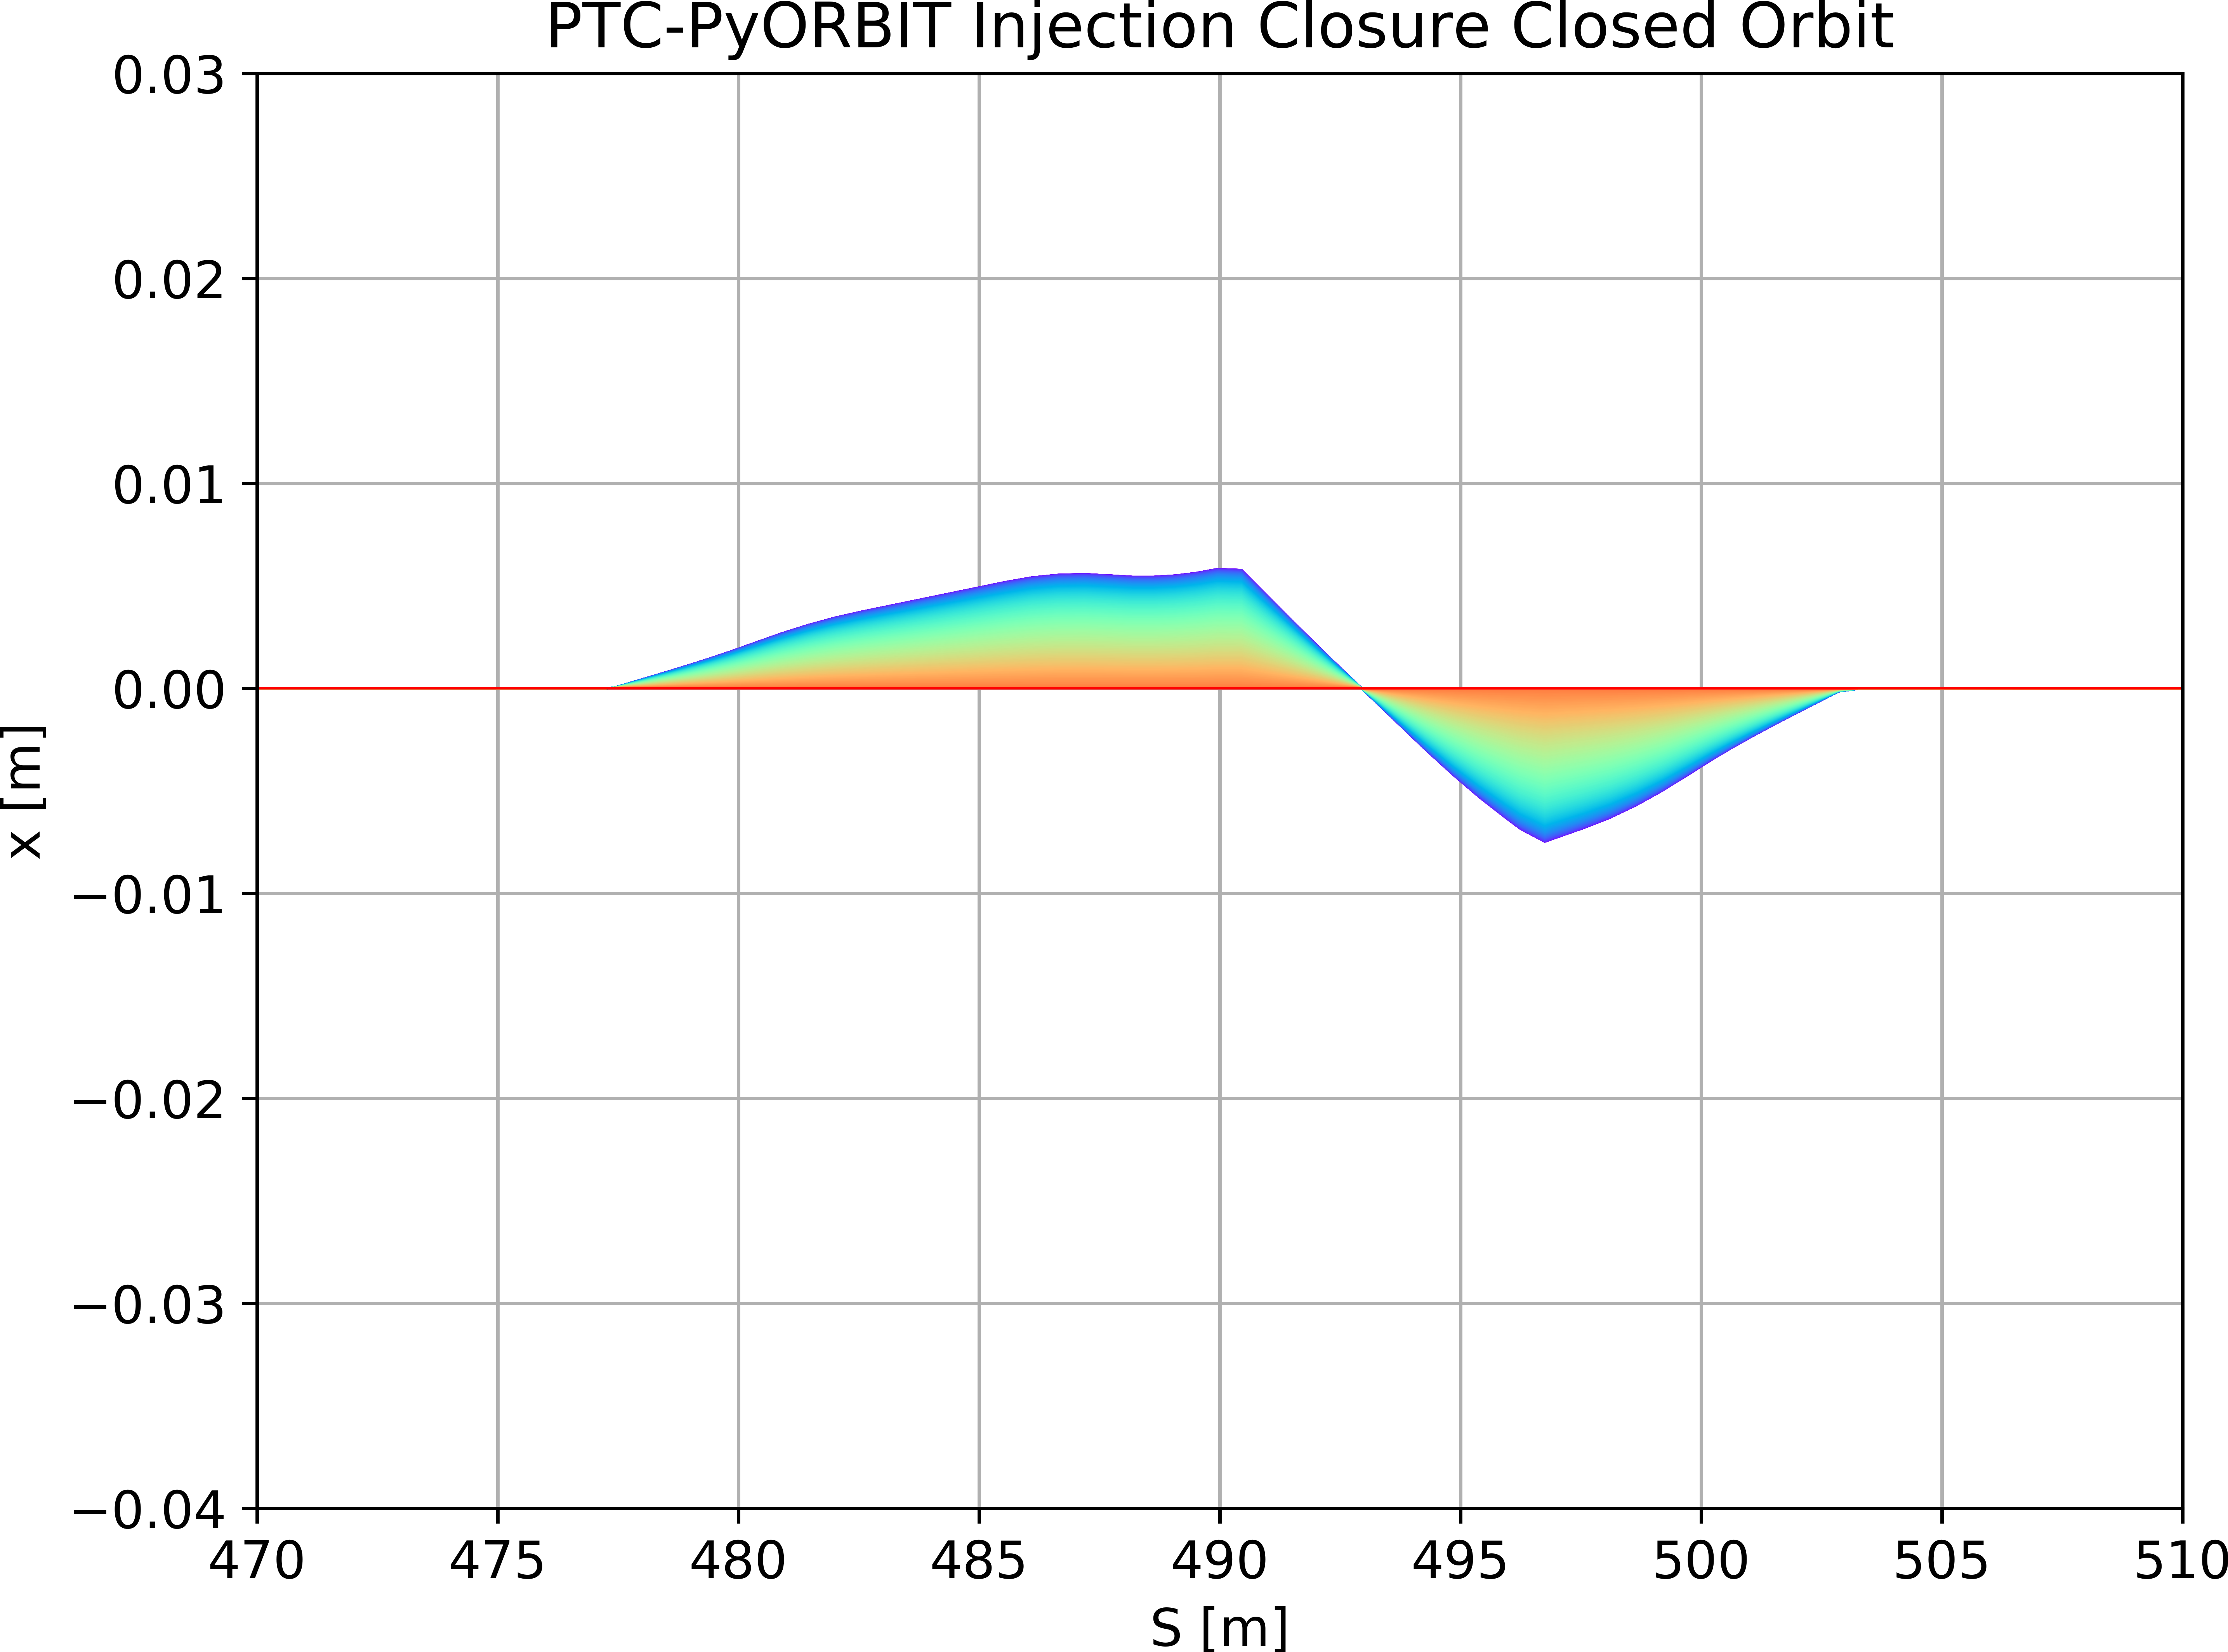
\includegraphics[width=0.3\textwidth]{No_Sext/03_SBEND/PTC-PyORBIT_Closed_Orbit03_SBEND_zoom.png}
            \caption{Horizontal closed orbit for split SBEND: MAD-X, PTC, PyORBIT.}
            \label{fig:03_CO_zoom}
        \end{figure}
    }
     \frame{
        \frametitle{QUADRUPOLE (as errors) Closed Orbit: Normalise PTC-PyORBIT table with length of element}
        Divide dipole component from MAD-X output table by length of element.
        
        \begin{figure}
            \centering
            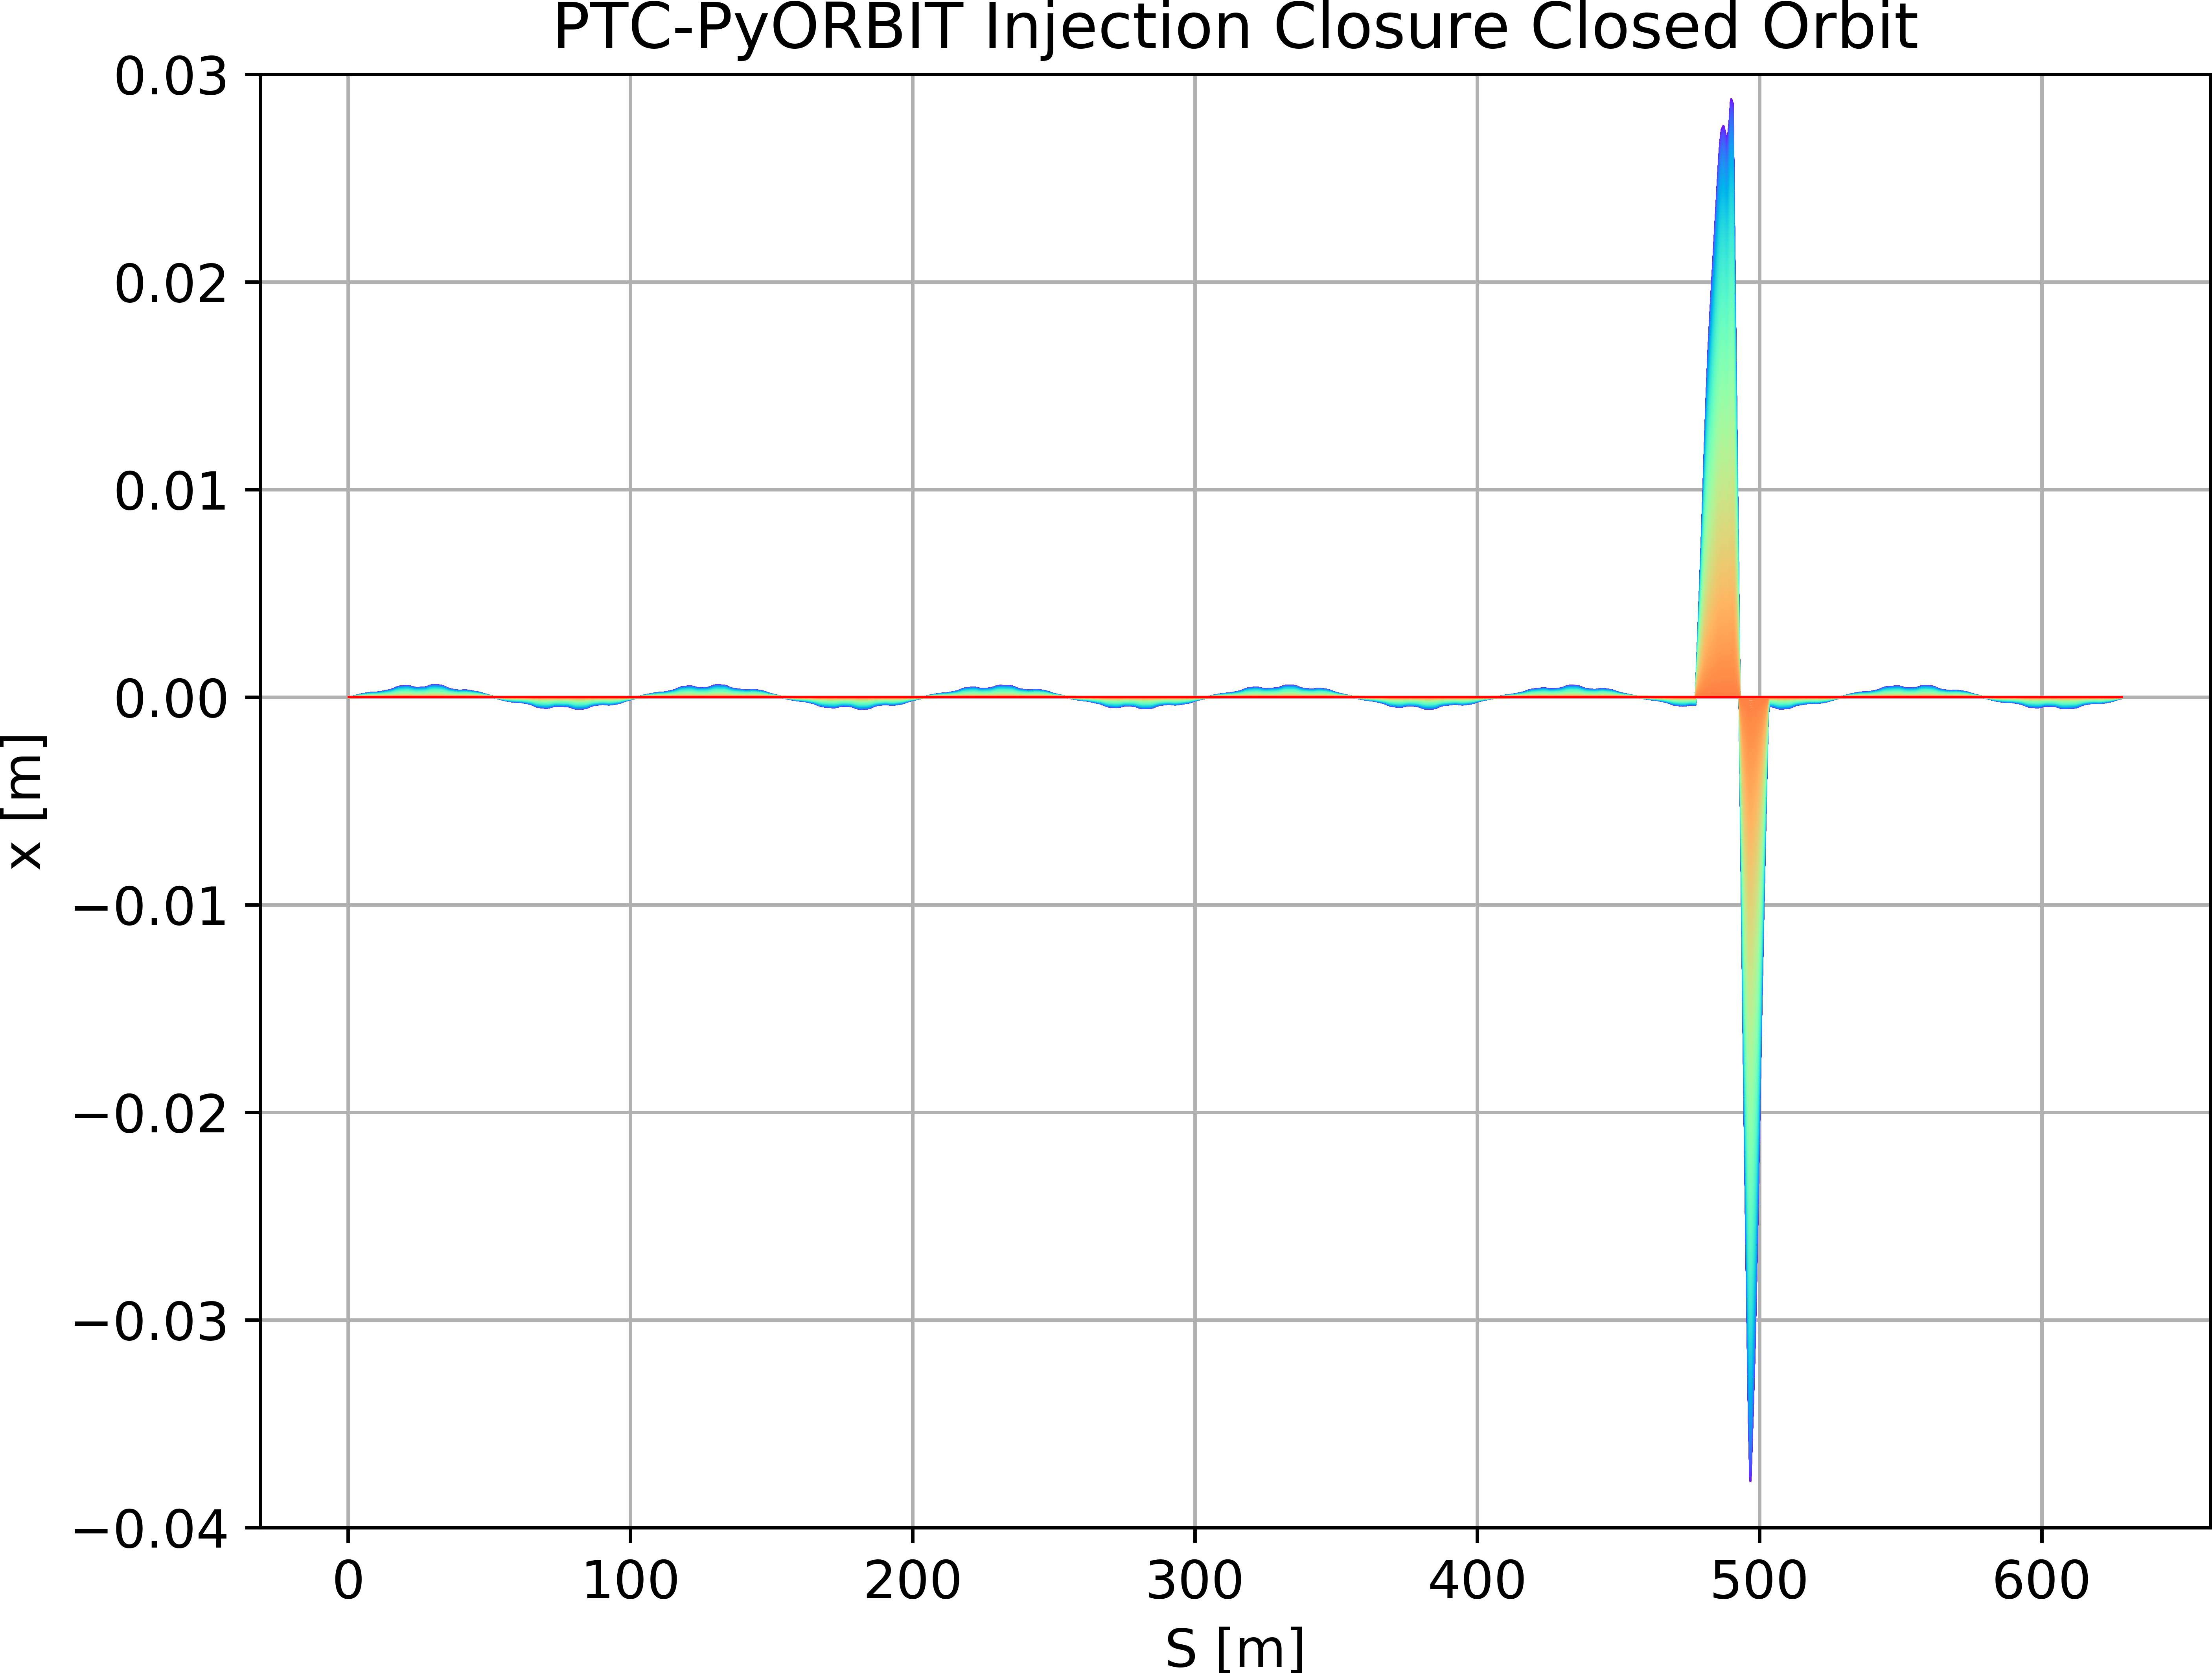
\includegraphics[width=0.3\textwidth]{No_Sext_Fudge/01_QUAD_f5/PTC-PyORBIT_Closed_Orbit02_QUADRUPOLE_fudge_5.png}~~~~~
             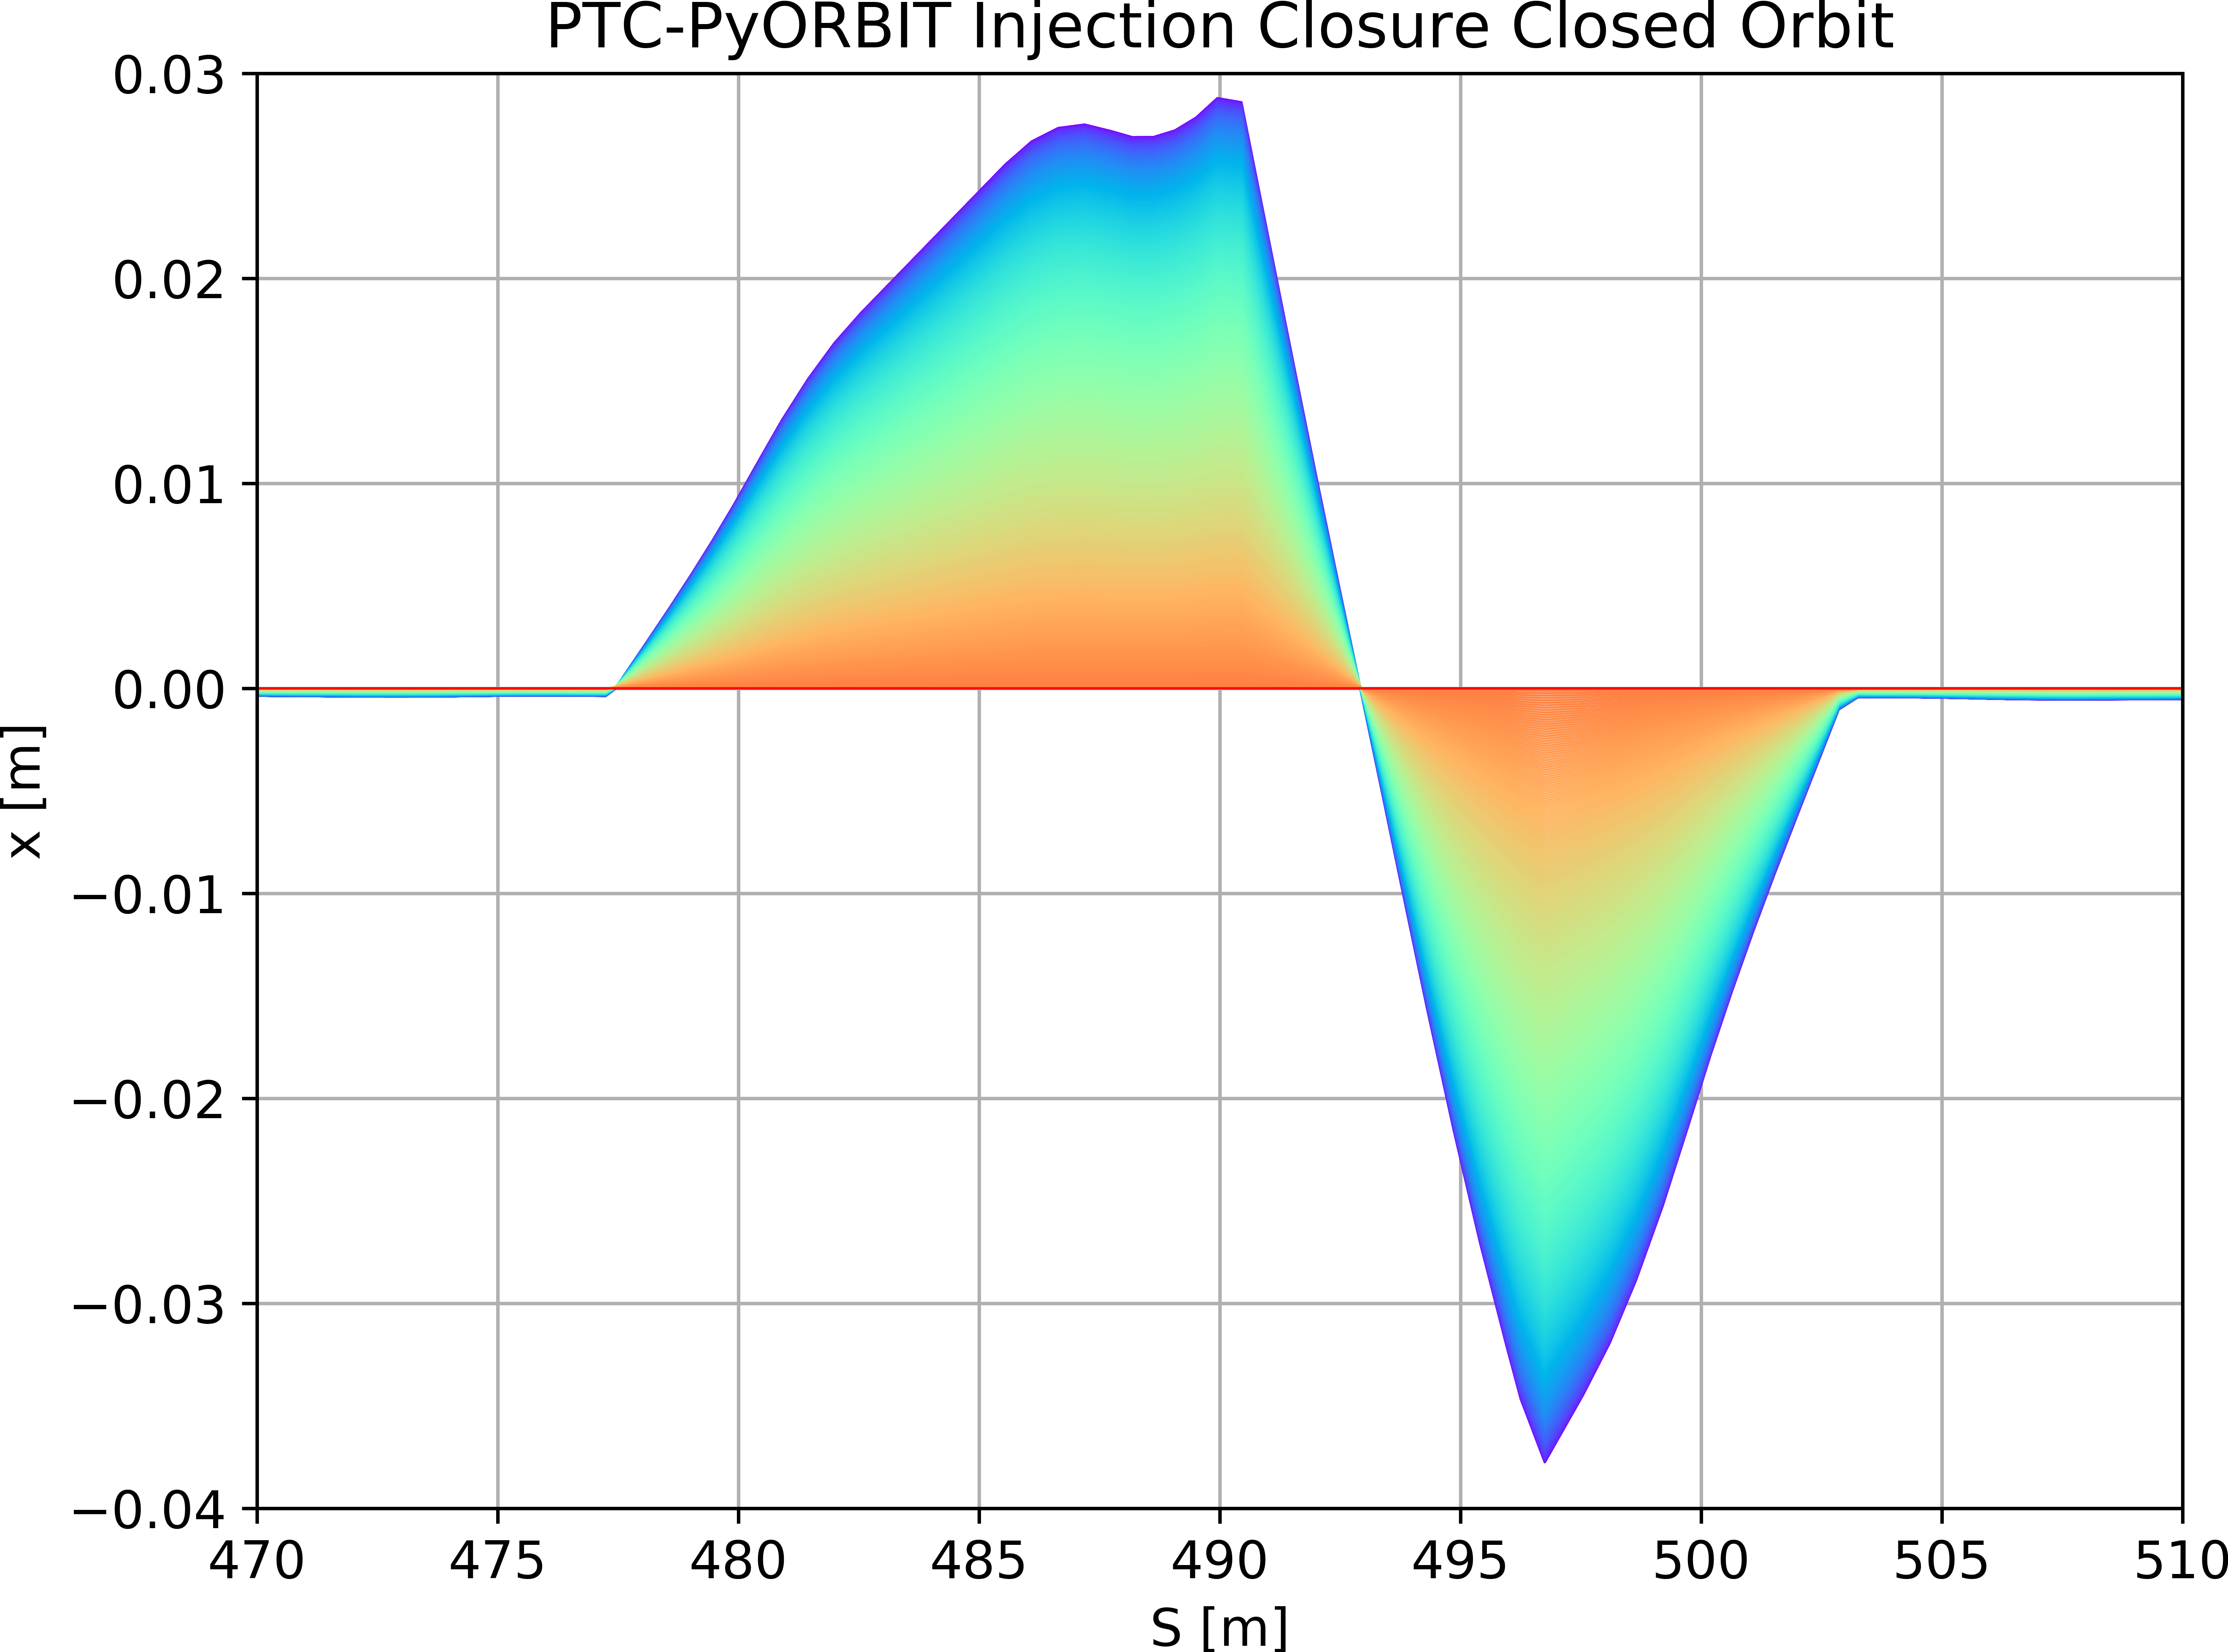
\includegraphics[width=0.3\textwidth]{No_Sext_Fudge/01_QUAD_f5/PTC-PyORBIT_Closed_Orbit02_QUADRUPOLE_fudge_5_zoom.png}
            \caption{Horizontal closed orbit for split SBEND: MAD-X, PTC, PyORBIT.}
            \label{fig:02_CO_fudge}
        \end{figure}
    }
    \frame{
        \frametitle{SBEND (as errors) Closed Orbit: Normalise PTC-PyORBIT table with length of element}
         Divide dipole component from MAD-X output table by length of element.
        \begin{figure}
            \centering
            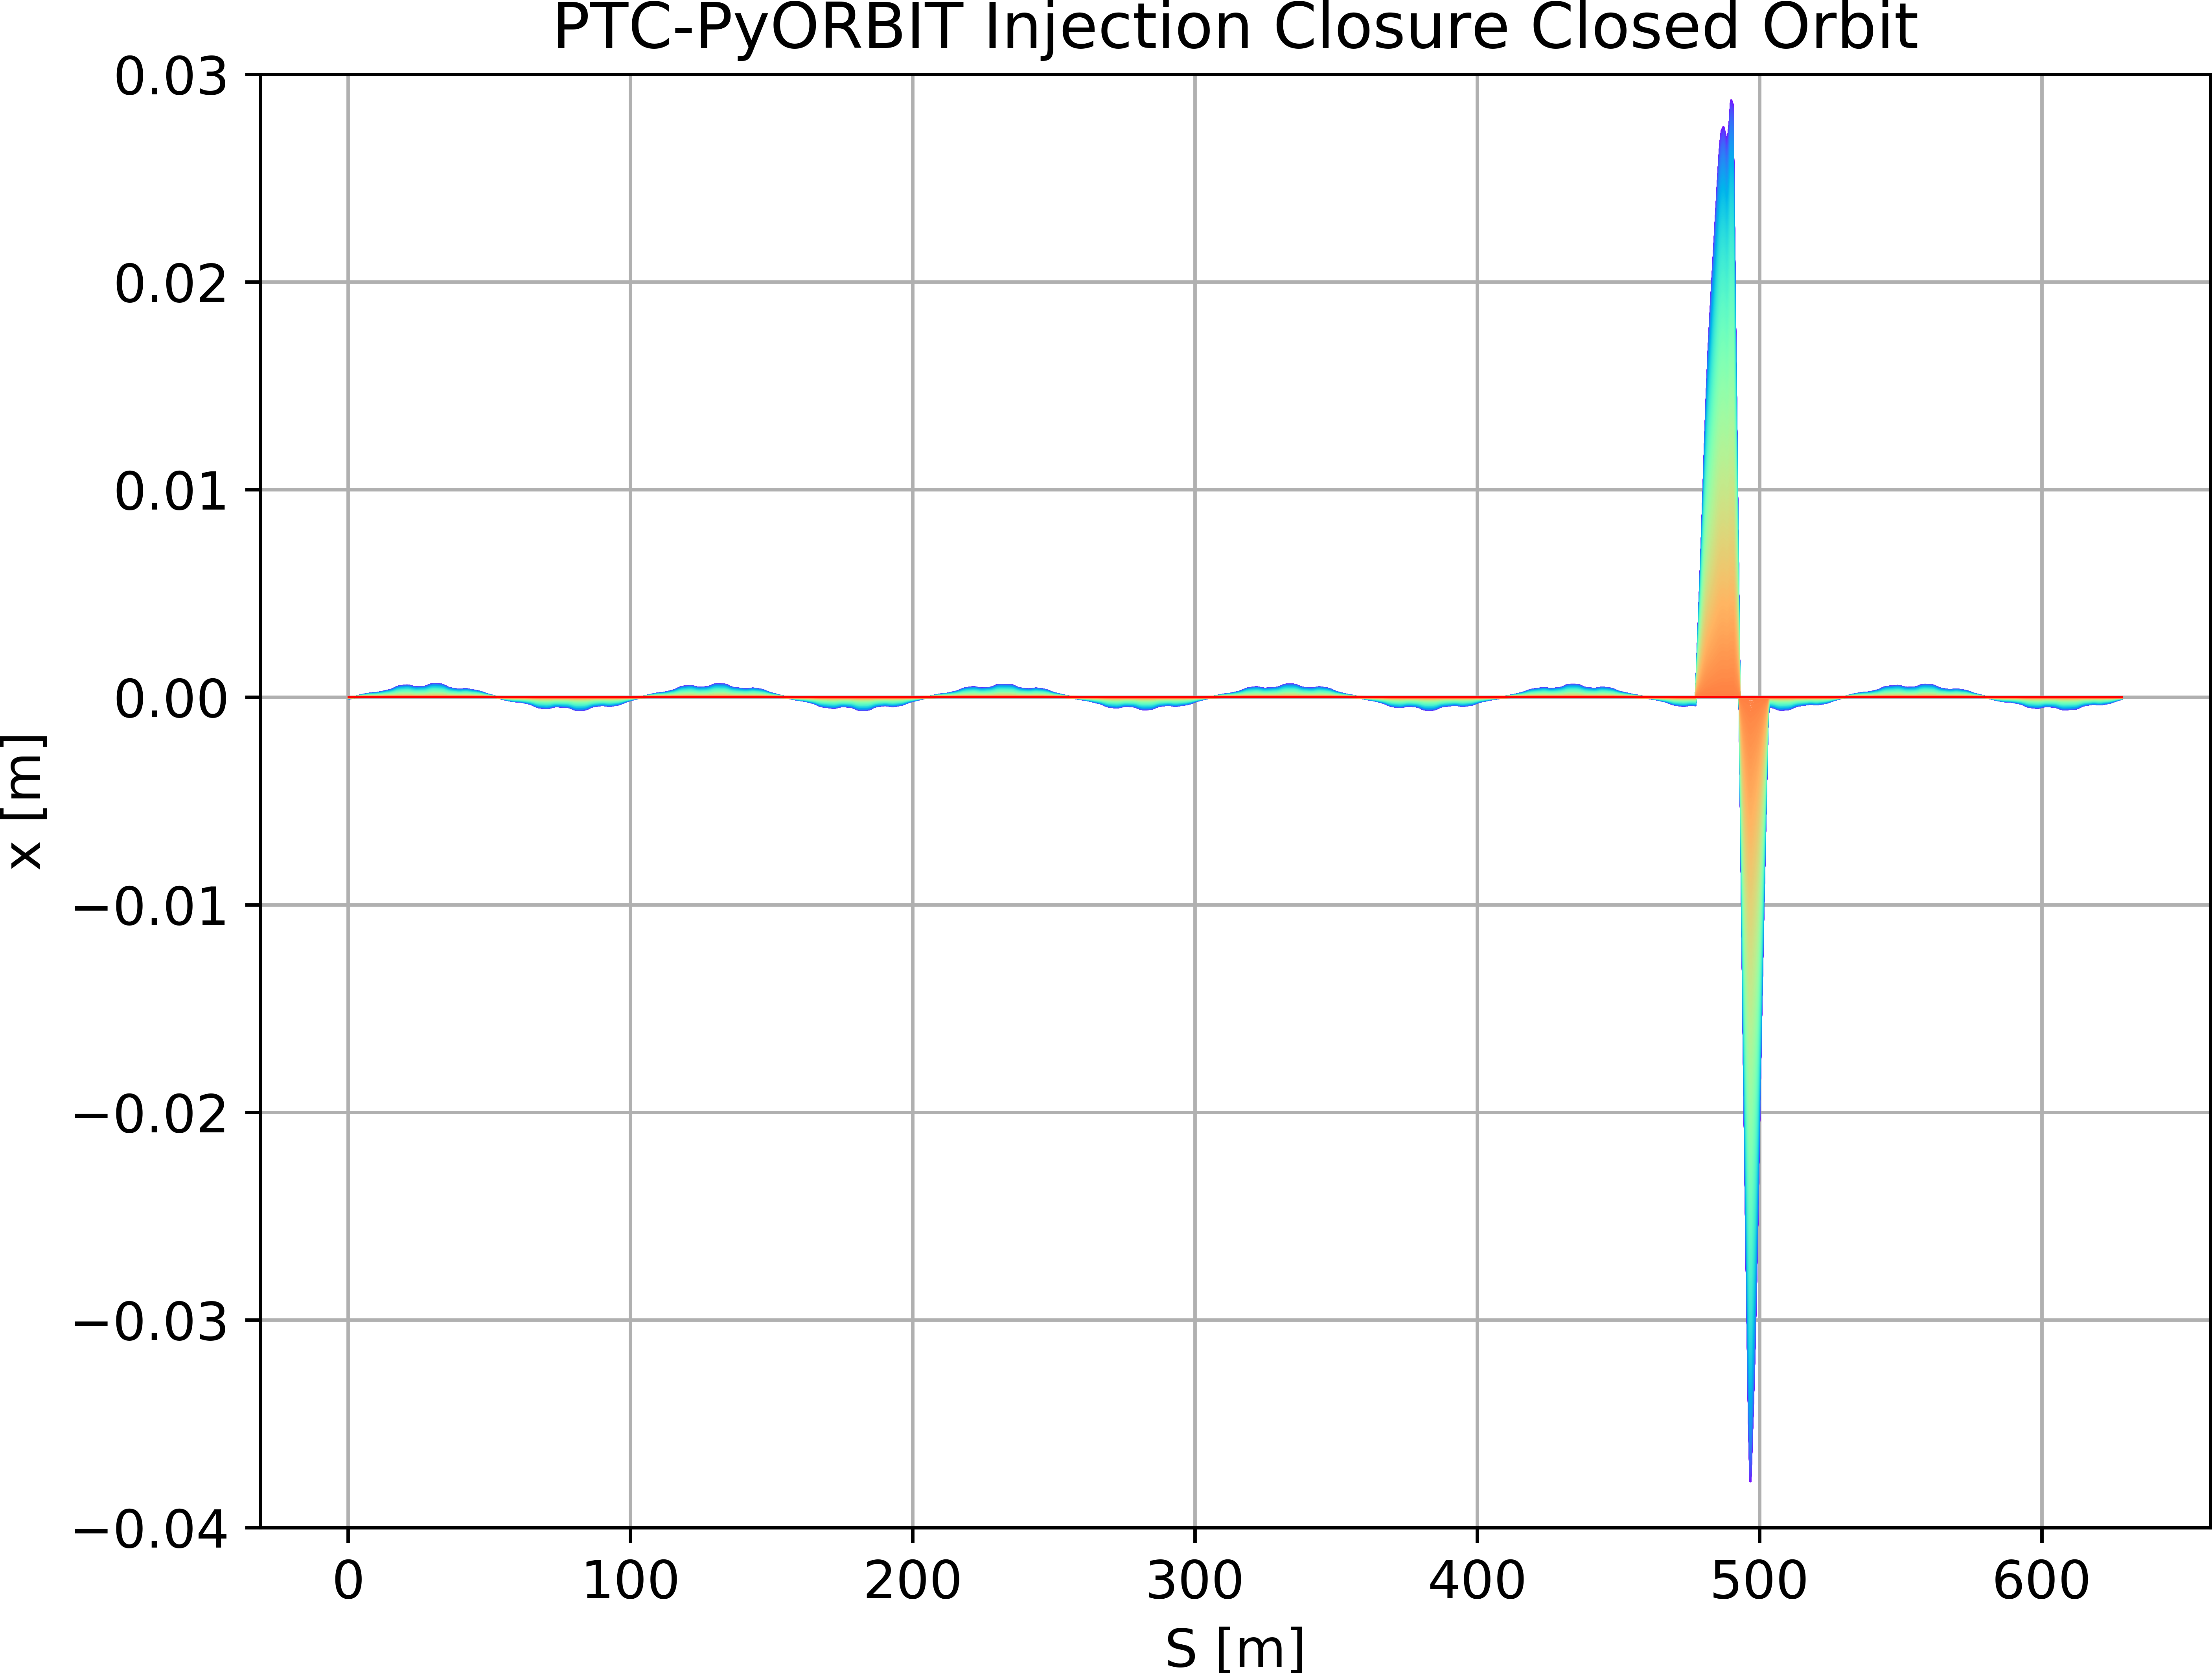
\includegraphics[width=0.3\textwidth]{No_Sext_Fudge/02_SBEND_f5/PTC-PyORBIT_Closed_Orbit03_SBEND_fudge_5.png}~~~~~
             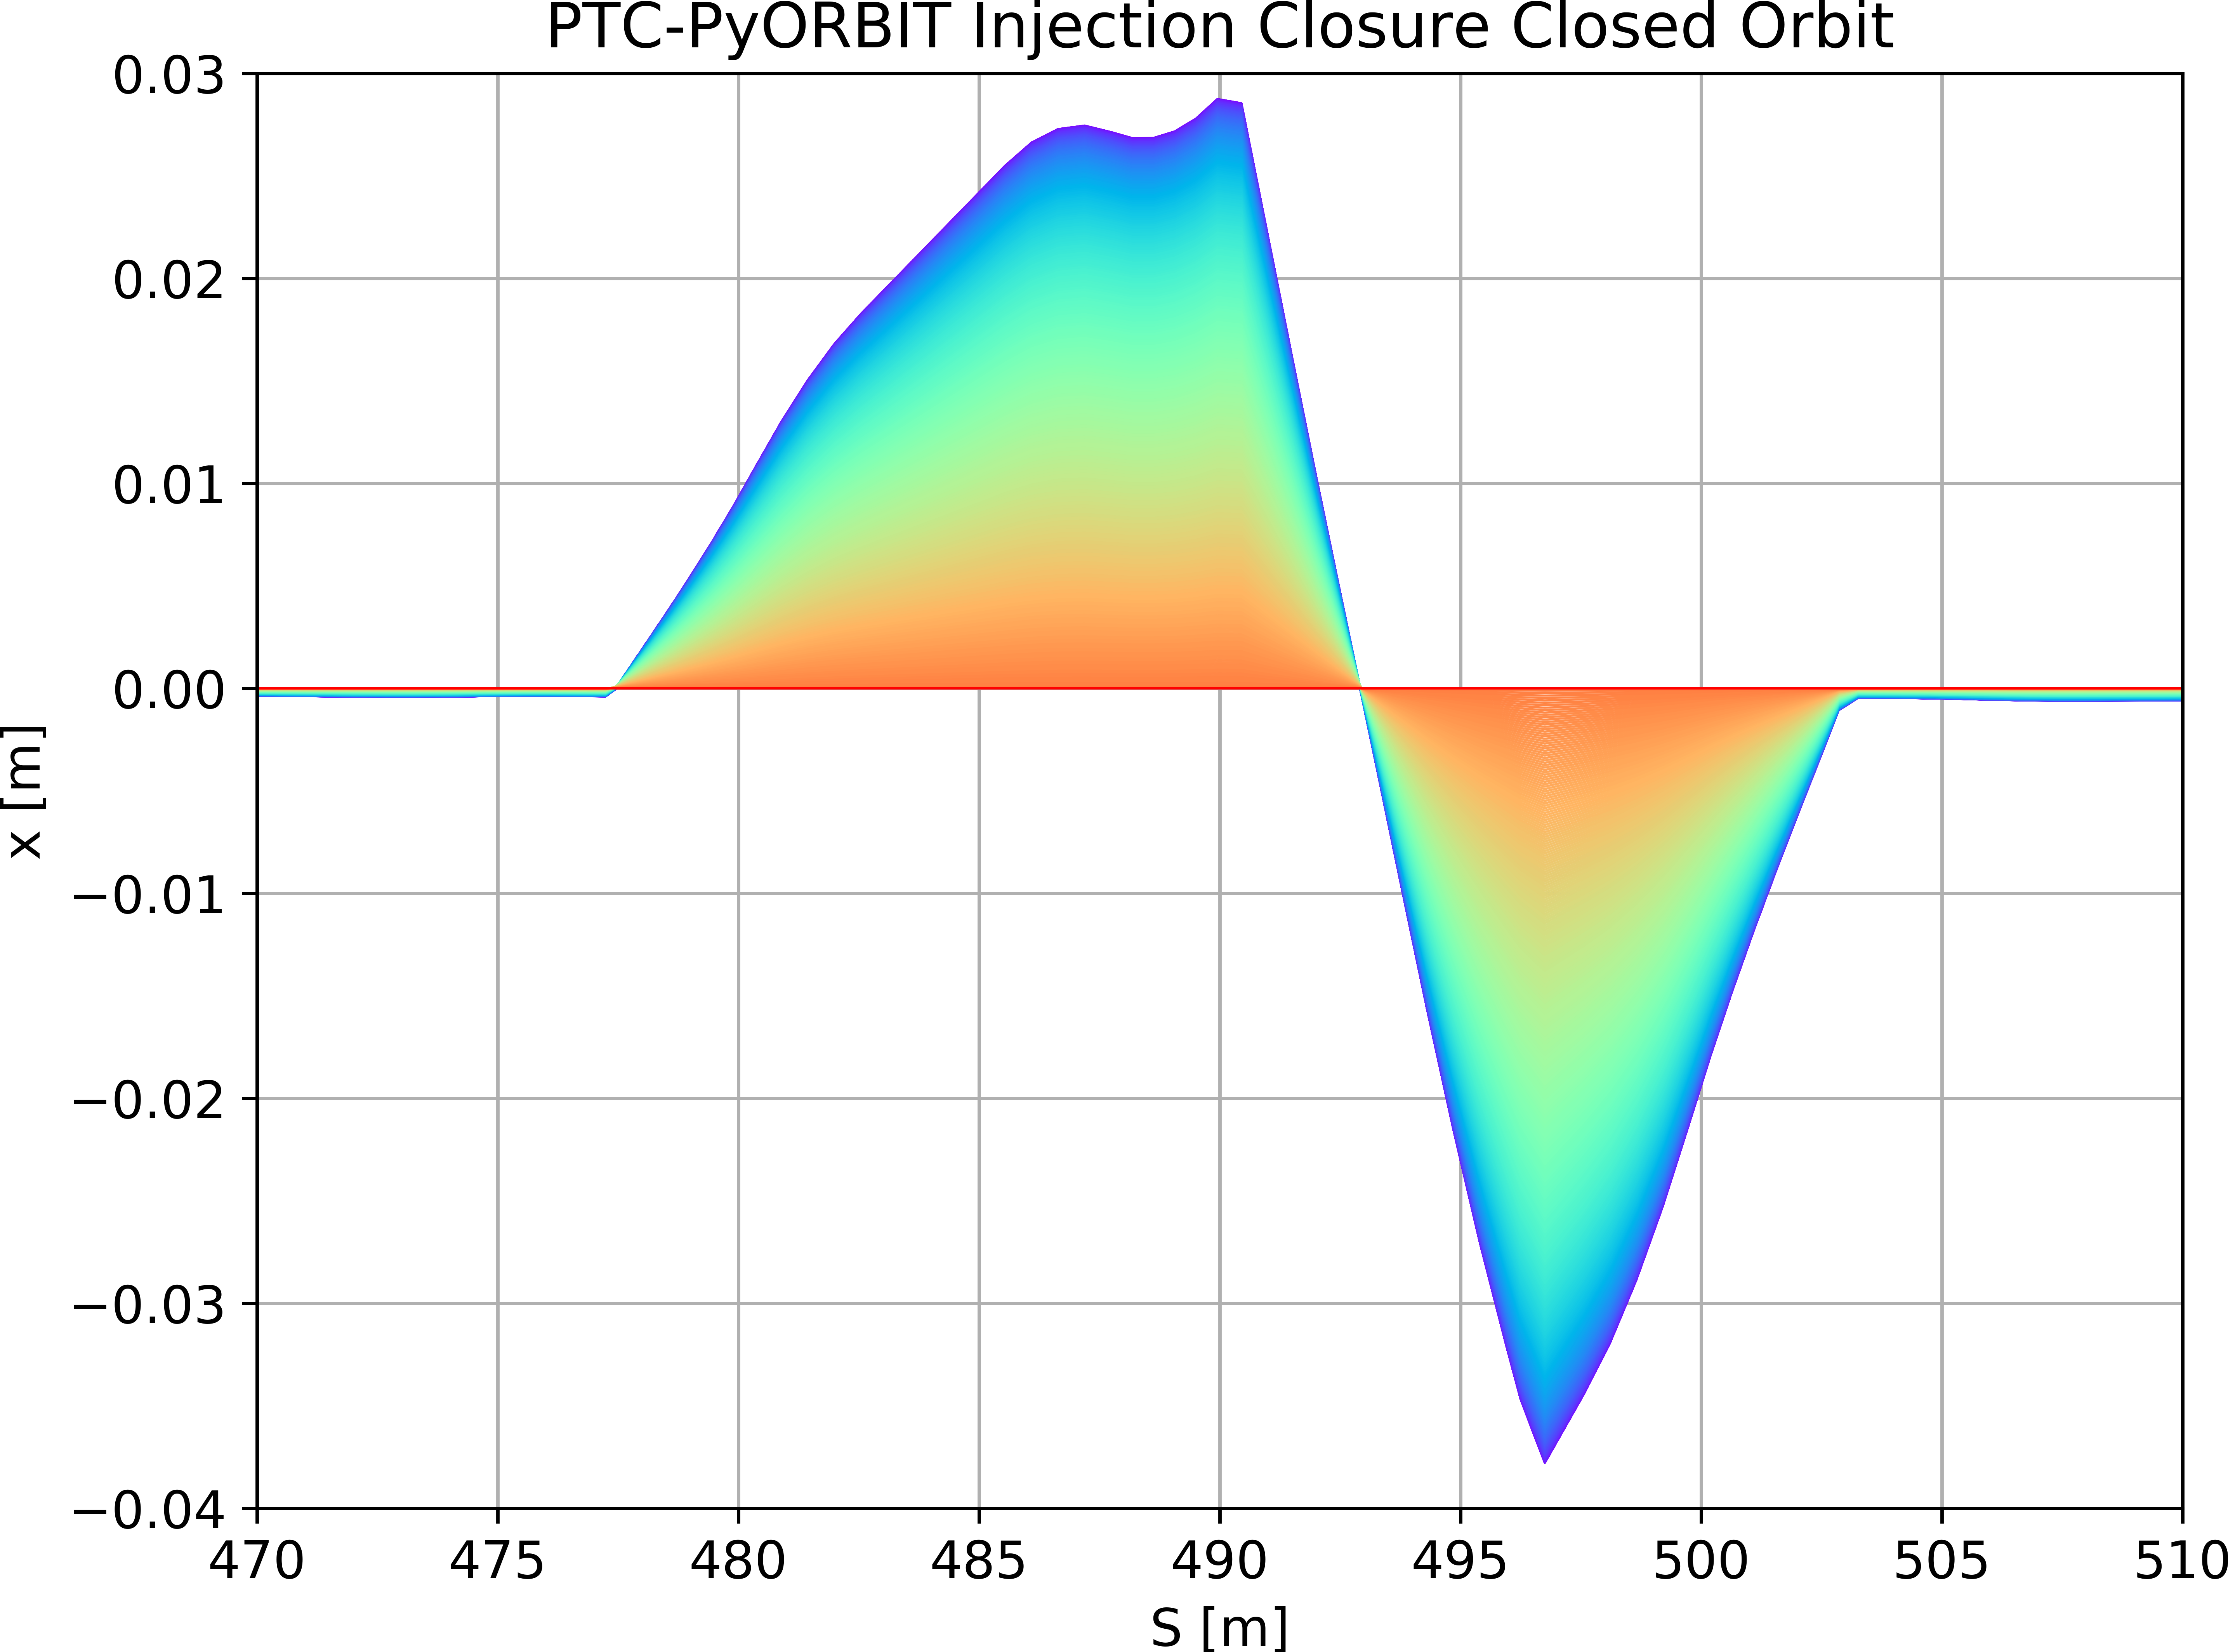
\includegraphics[width=0.3\textwidth]{No_Sext_Fudge/02_SBEND_f5/PTC-PyORBIT_Closed_Orbit03_SBEND_fudge_5_zoom.png}
            \caption{Horizontal closed orbit for split SBEND: MAD-X, PTC, PyORBIT.}
            \label{fig:02_CO_fudge}
        \end{figure}
    }
    
    \frame{
        \frametitle{Issues}
        \begin{itemize}
            \item Make sure to update PTC and PyORBIT every turn.
            \item Include calls to correct PTC files (energize lattice, update twiss, read final settings etc).
            \item Unknown environment bug on LXPlus and HPC-Batch: causes simulation to run without updating PTC every turn - for unknown reason. Now seems to work - not satisfied with not knowing more - will keep an eye out for future wierdness.
            \item Dipole component needed to be normalised when used in QUADRUPOLE and SBEND methods.
        \end{itemize}
    }

 
        
    \section{PS Transfer}
    
    \frame{
        \frametitle{Goals}
        
        \begin{itemize}
            \item To investigate the space charge contribution to beam envelope oscillations observed in the PS immediately after injection.
            \item Reproduce measurements performed using BGI and SEM Grids in PTC-PyORBIT in order to understand the contribution of space charge.
        \end{itemize}
    }
    
    \frame{
        \frametitle{Current Plan}
        
        \begin{itemize}
            \item Start with matched distribution and track without space charge.
            \item Add dispersion mismatch as constant factor (will obtain parameterised values from Selim/Matthew soon).
            \item Start with PTC TWISS to match distribution, later use end of transfer line values transported to BGI/SEM position (to be provided by Selim/Matthew).
        \end{itemize}
        
        Note: all simulations run at the nominal working point of (Q$_x$, Q$_y$) = (6.21, 6.24).
    }
    
    \frame{
        \frametitle{Matched Distribution}
        
        \begin{block}{No Space Charge} Mismatch of factor 0\% and +10\%.
        \end{block}
        
        \begin{itemize}
            \item Had to correct units of dE (factor 1E3).
            \item Matching not correct.
            \item Abandon and use tomo distribution.
        \end{itemize}
    }
    
    \frame{
        \frametitle{Matched Distribution Longitudinal Motion}
        
        \begin{figure}
            \centering
            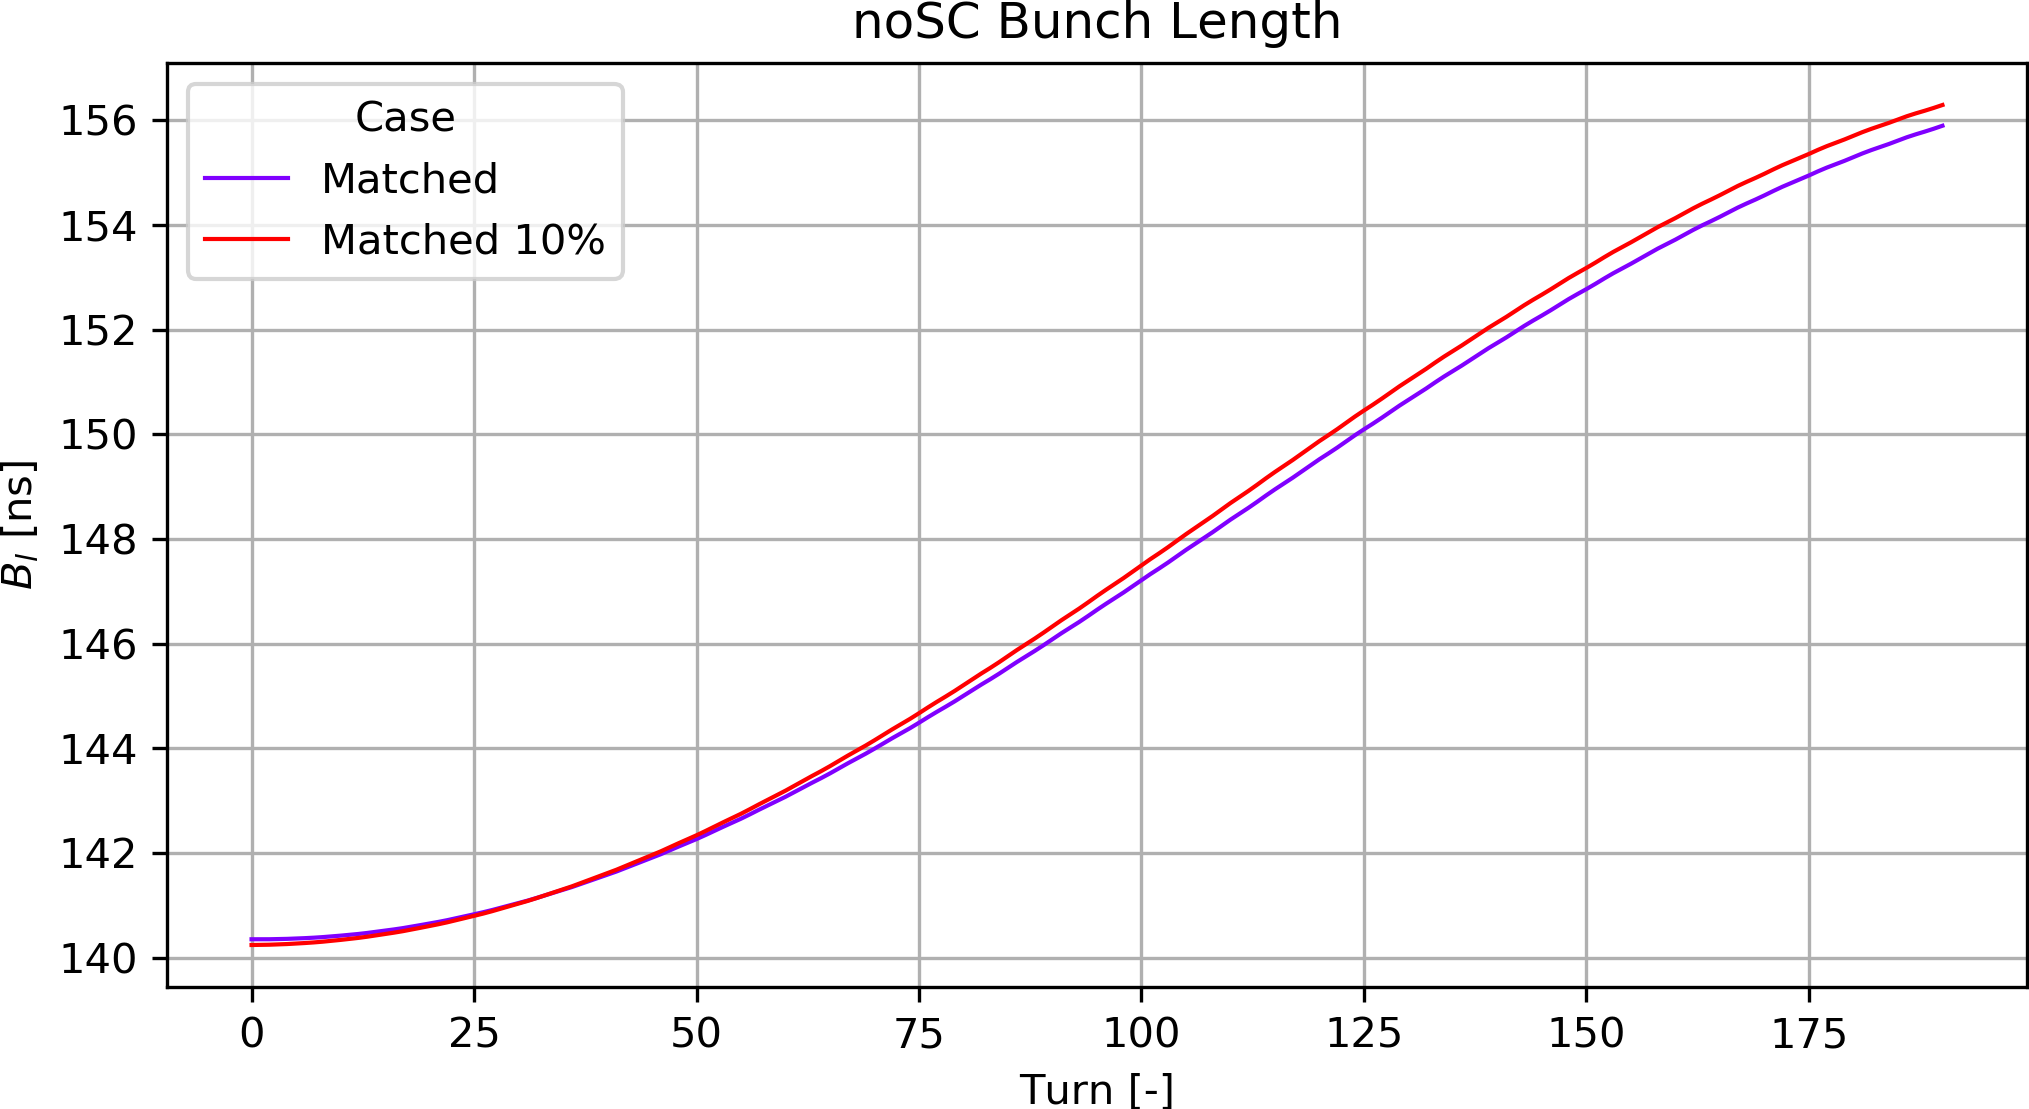
\includegraphics[width=0.45\textwidth]{PS_Transfer/Matched/SEM_Matched_noSC_bunchlength.png}~~~~
            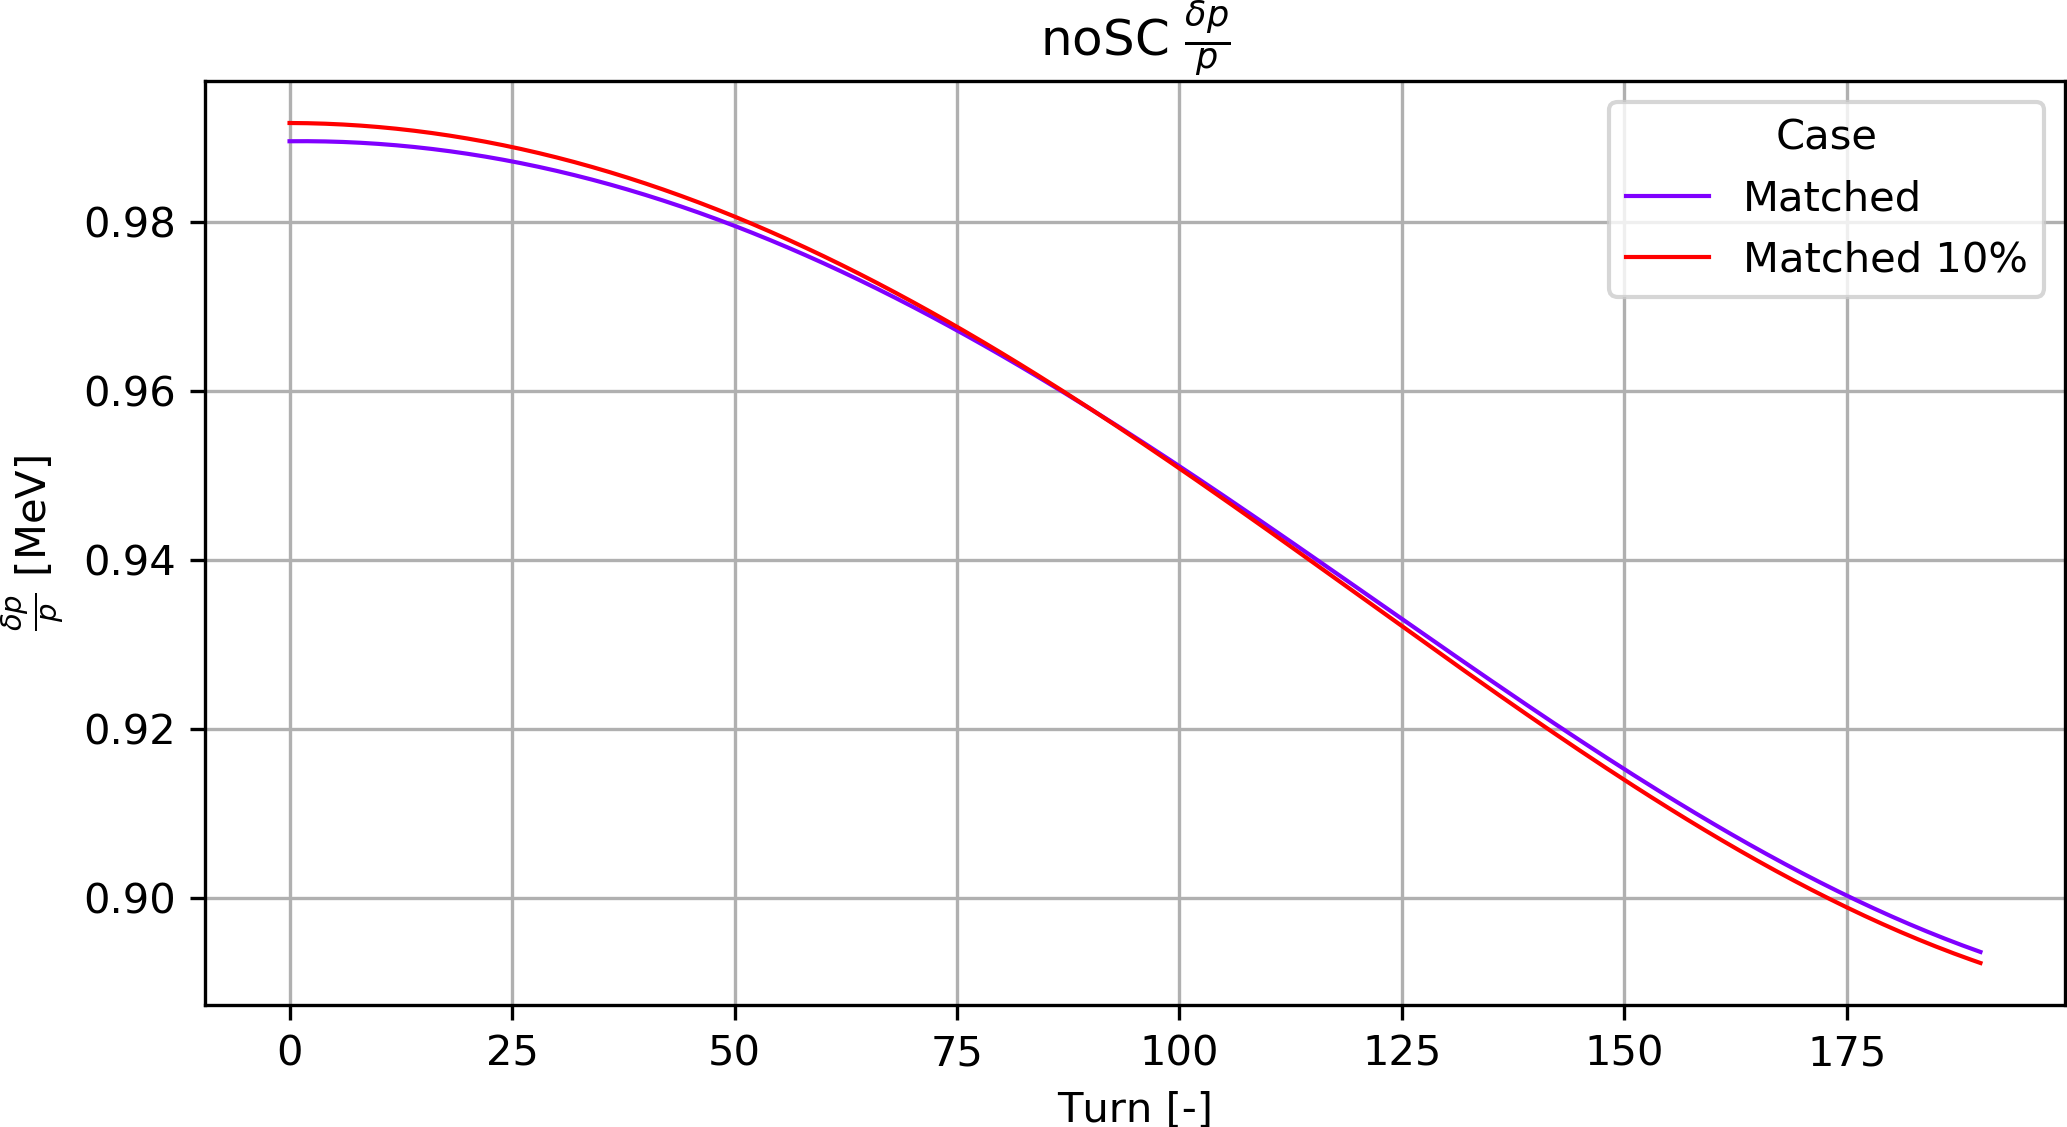
\includegraphics[width=0.45\textwidth]{PS_Transfer/Matched/SEM_Matched_noSC_dpp_rms.png}
            \caption{Longitudinal motion for \texttt{matched} distribution: oscillations larger than expected - indicates mismatch.}
            \label{fig:matched_longitudinal}
        \end{figure}
    }
    
    \frame{
        \frametitle{Matched Distribution Horizontal Dispersion}
        
        \begin{figure}
            \centering
            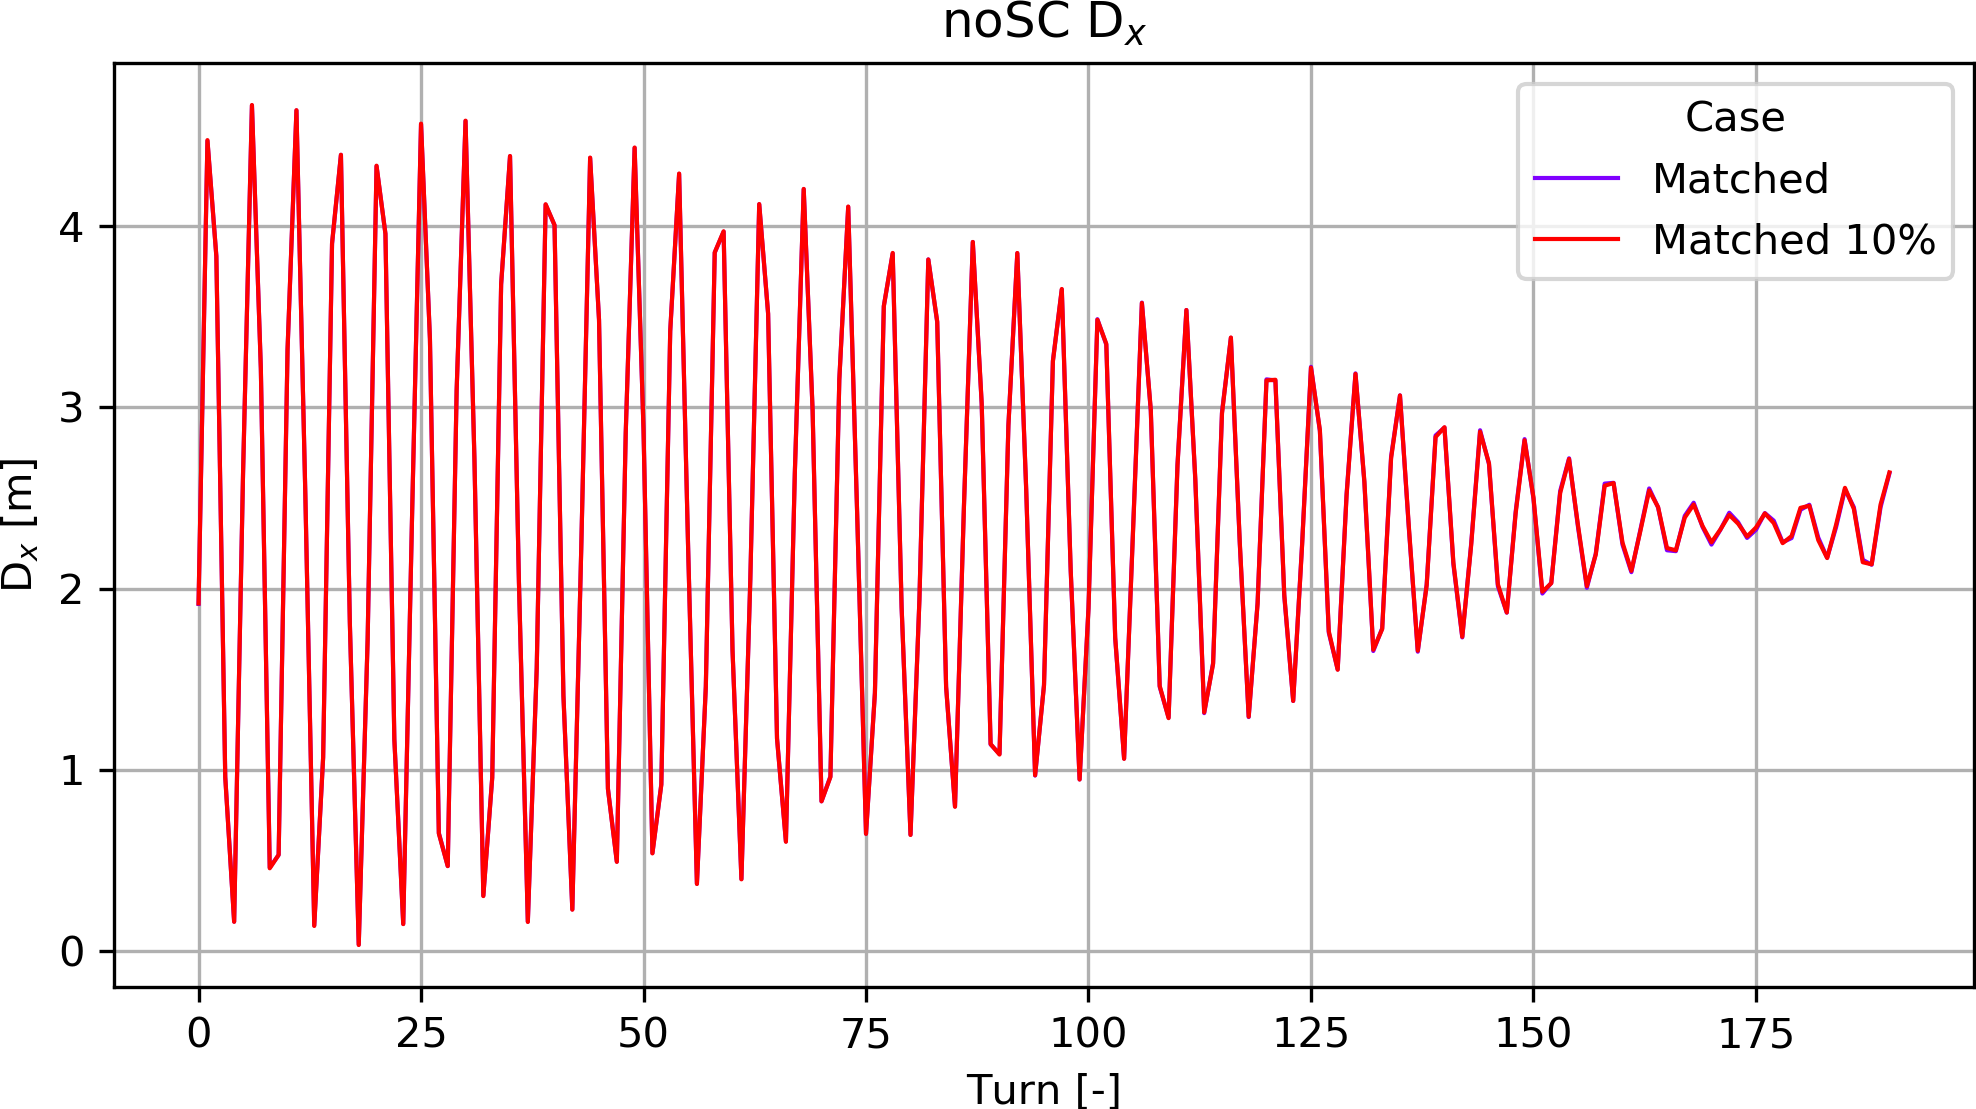
\includegraphics[width=0.45\textwidth]{PS_Transfer/Matched/SEM_Matched_noSC_D_x.png}~~~~
            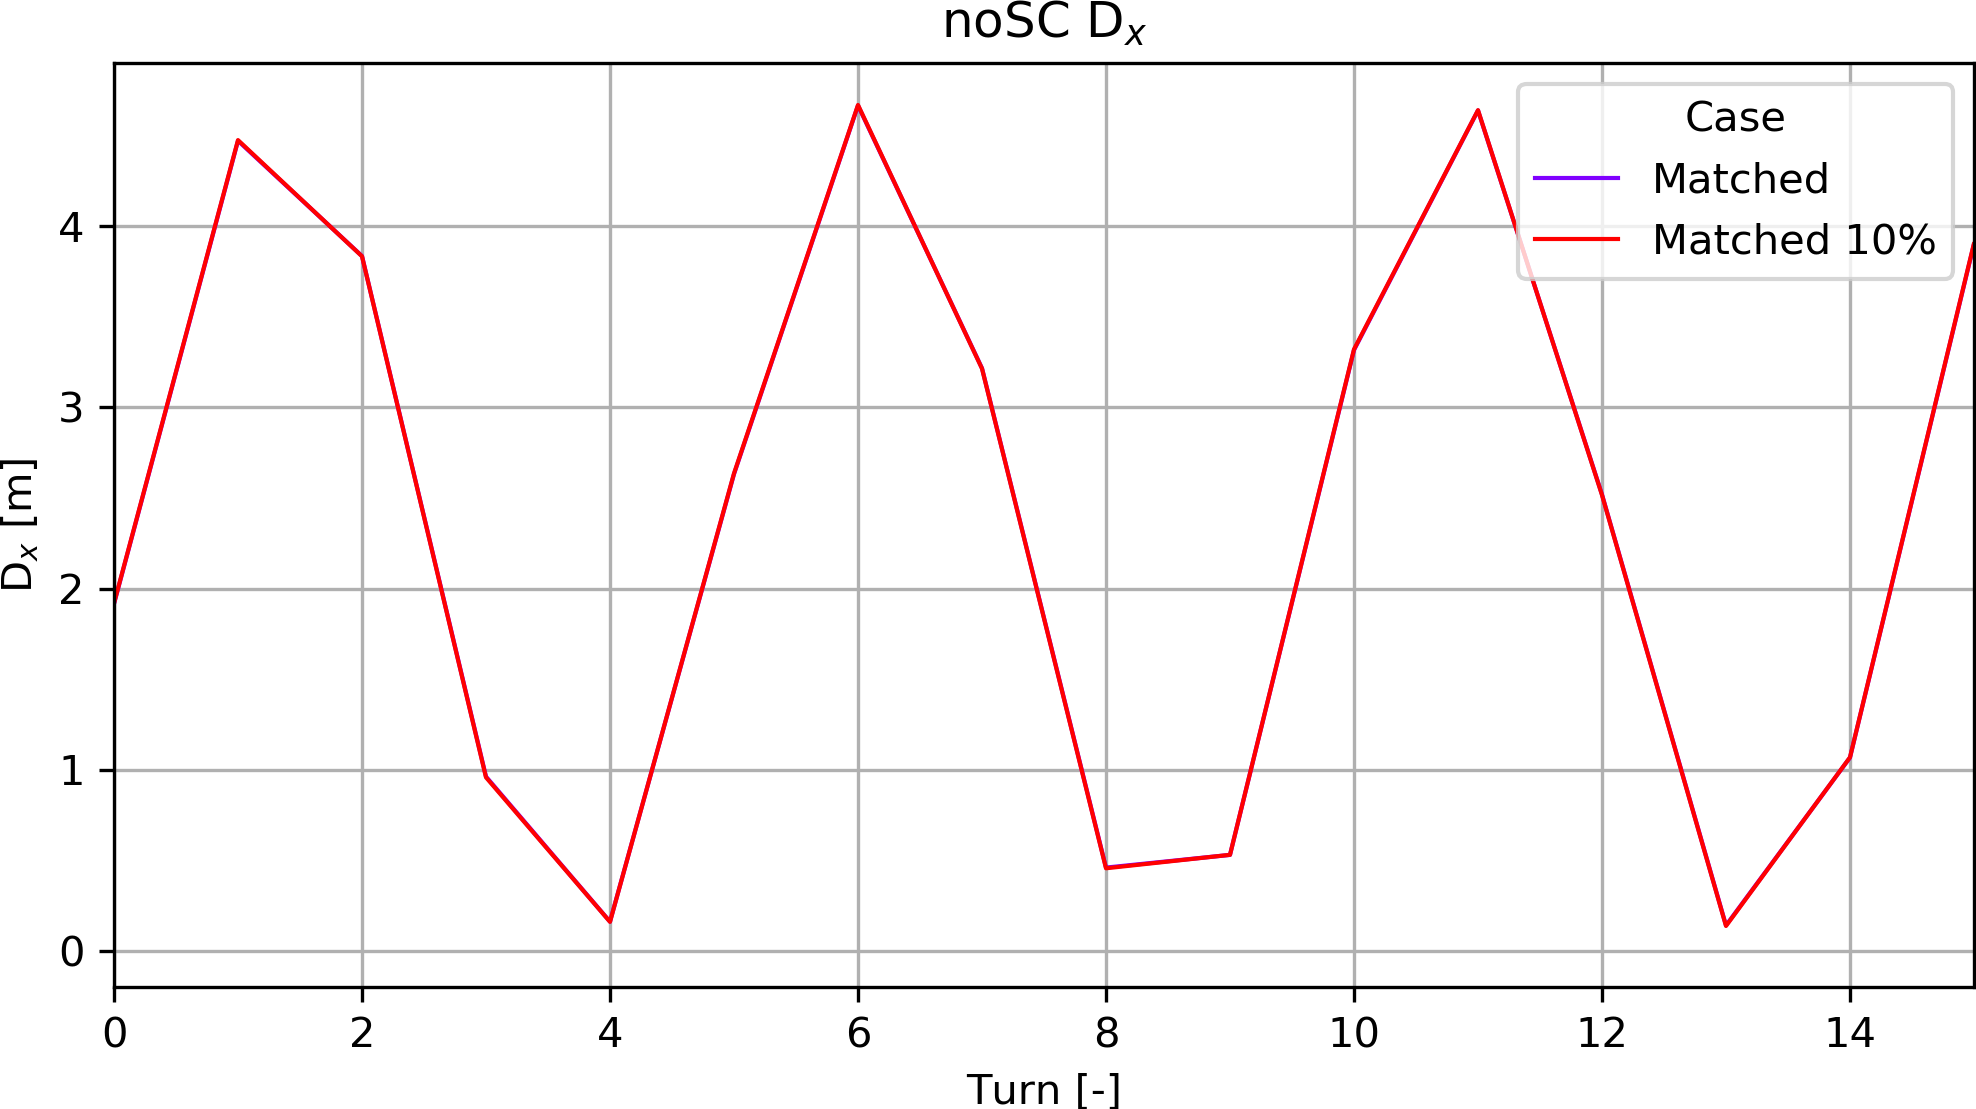
\includegraphics[width=0.45\textwidth]{PS_Transfer/Matched/SEM_Matched_noSC_zoom_D_x.png}
            \caption{Horizontal dispersion for \texttt{matched} distribution: 10\% mismatch identical to 0\% mismatch - indicates existing mismatch already larger than 10\%.}
            \label{fig:matched_dispersion}
        \end{figure}
    }
    
    \frame{
        \frametitle{Matched Distribution Emittances}
        
        \begin{figure}
            \centering
            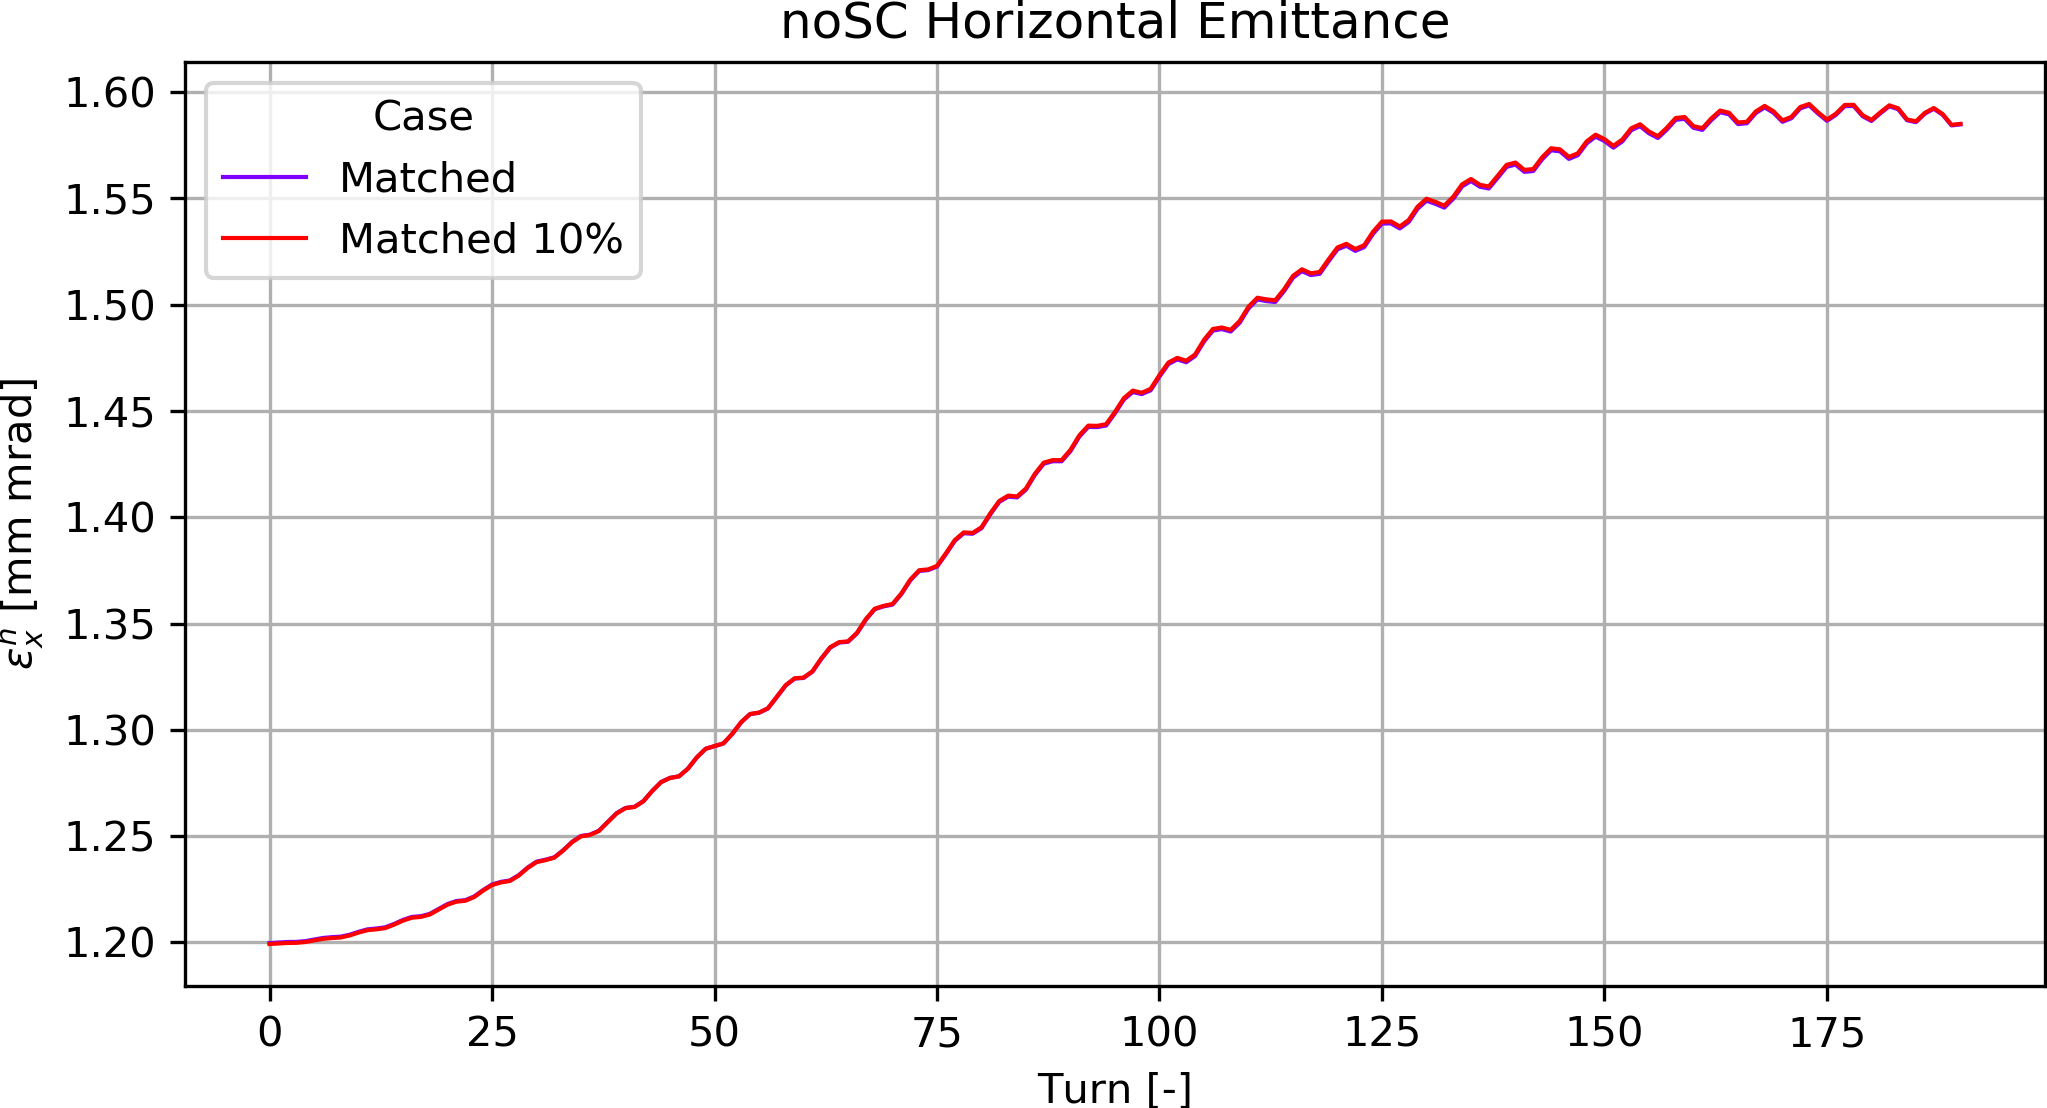
\includegraphics[width=0.45\textwidth]{PS_Transfer/Matched/SEM_Matched_noSC_epsn_x.png}~~~~
            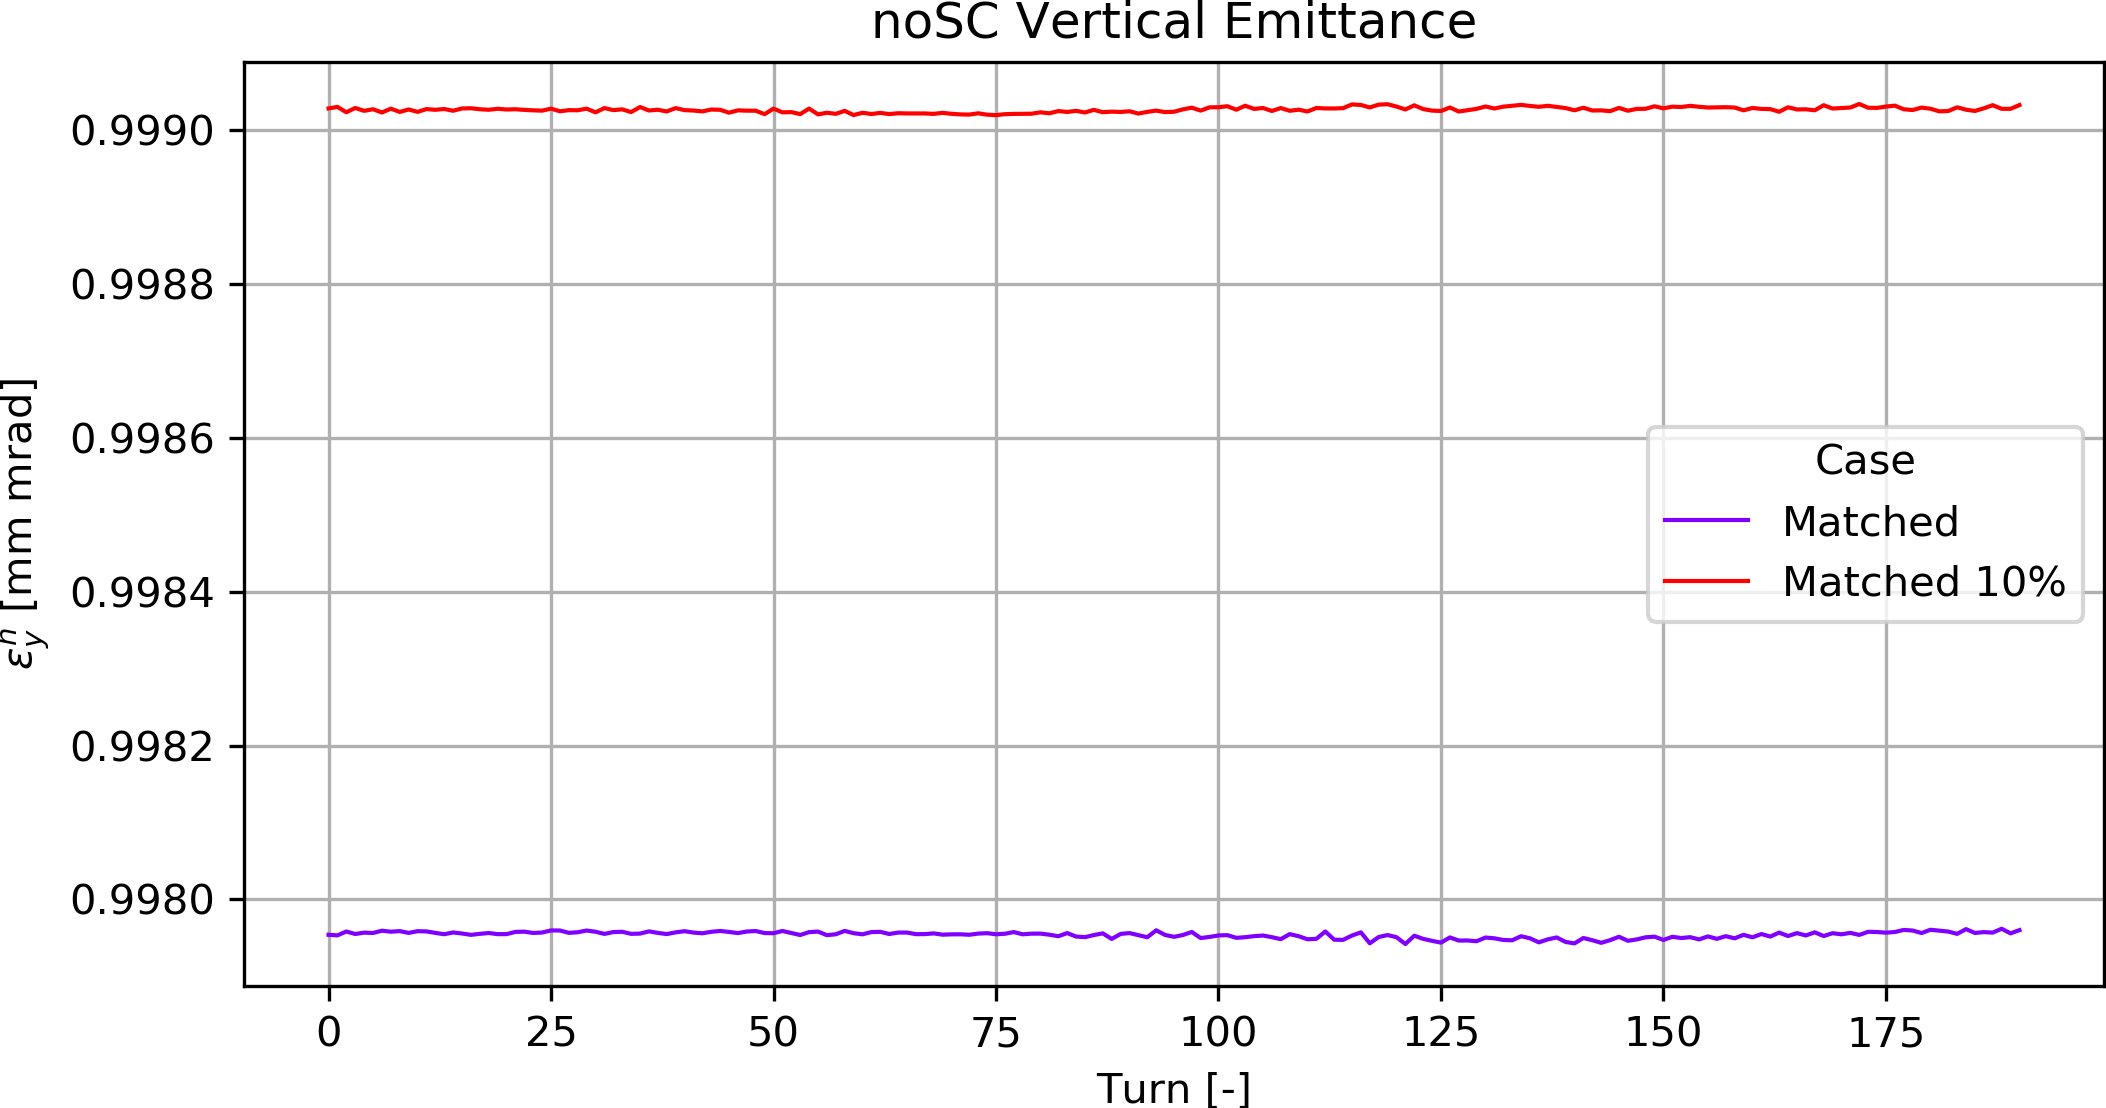
\includegraphics[width=0.45\textwidth]{PS_Transfer/Matched/SEM_Matched_noSC_epsn_y.png}
            \caption{Emittances for \texttt{matched} distribution: 10\% mismatch identical to 0\% mismatch - indicates existing mismatch already larger than 10\%.}
            \label{fig:matched_emittances}
        \end{figure}
    }
    
    \frame{
        \frametitle{Tomo Distribution}
        \begin{block}{No Space Charge} Mismatch of factor 0\%, +10\%, +20\%, and +30\%.
        \end{block}
    }
    
      \frame{
        \frametitle{Tomo Distribution Longitudinal Motion (No Space Charge)}
        
        \begin{figure}
            \centering
            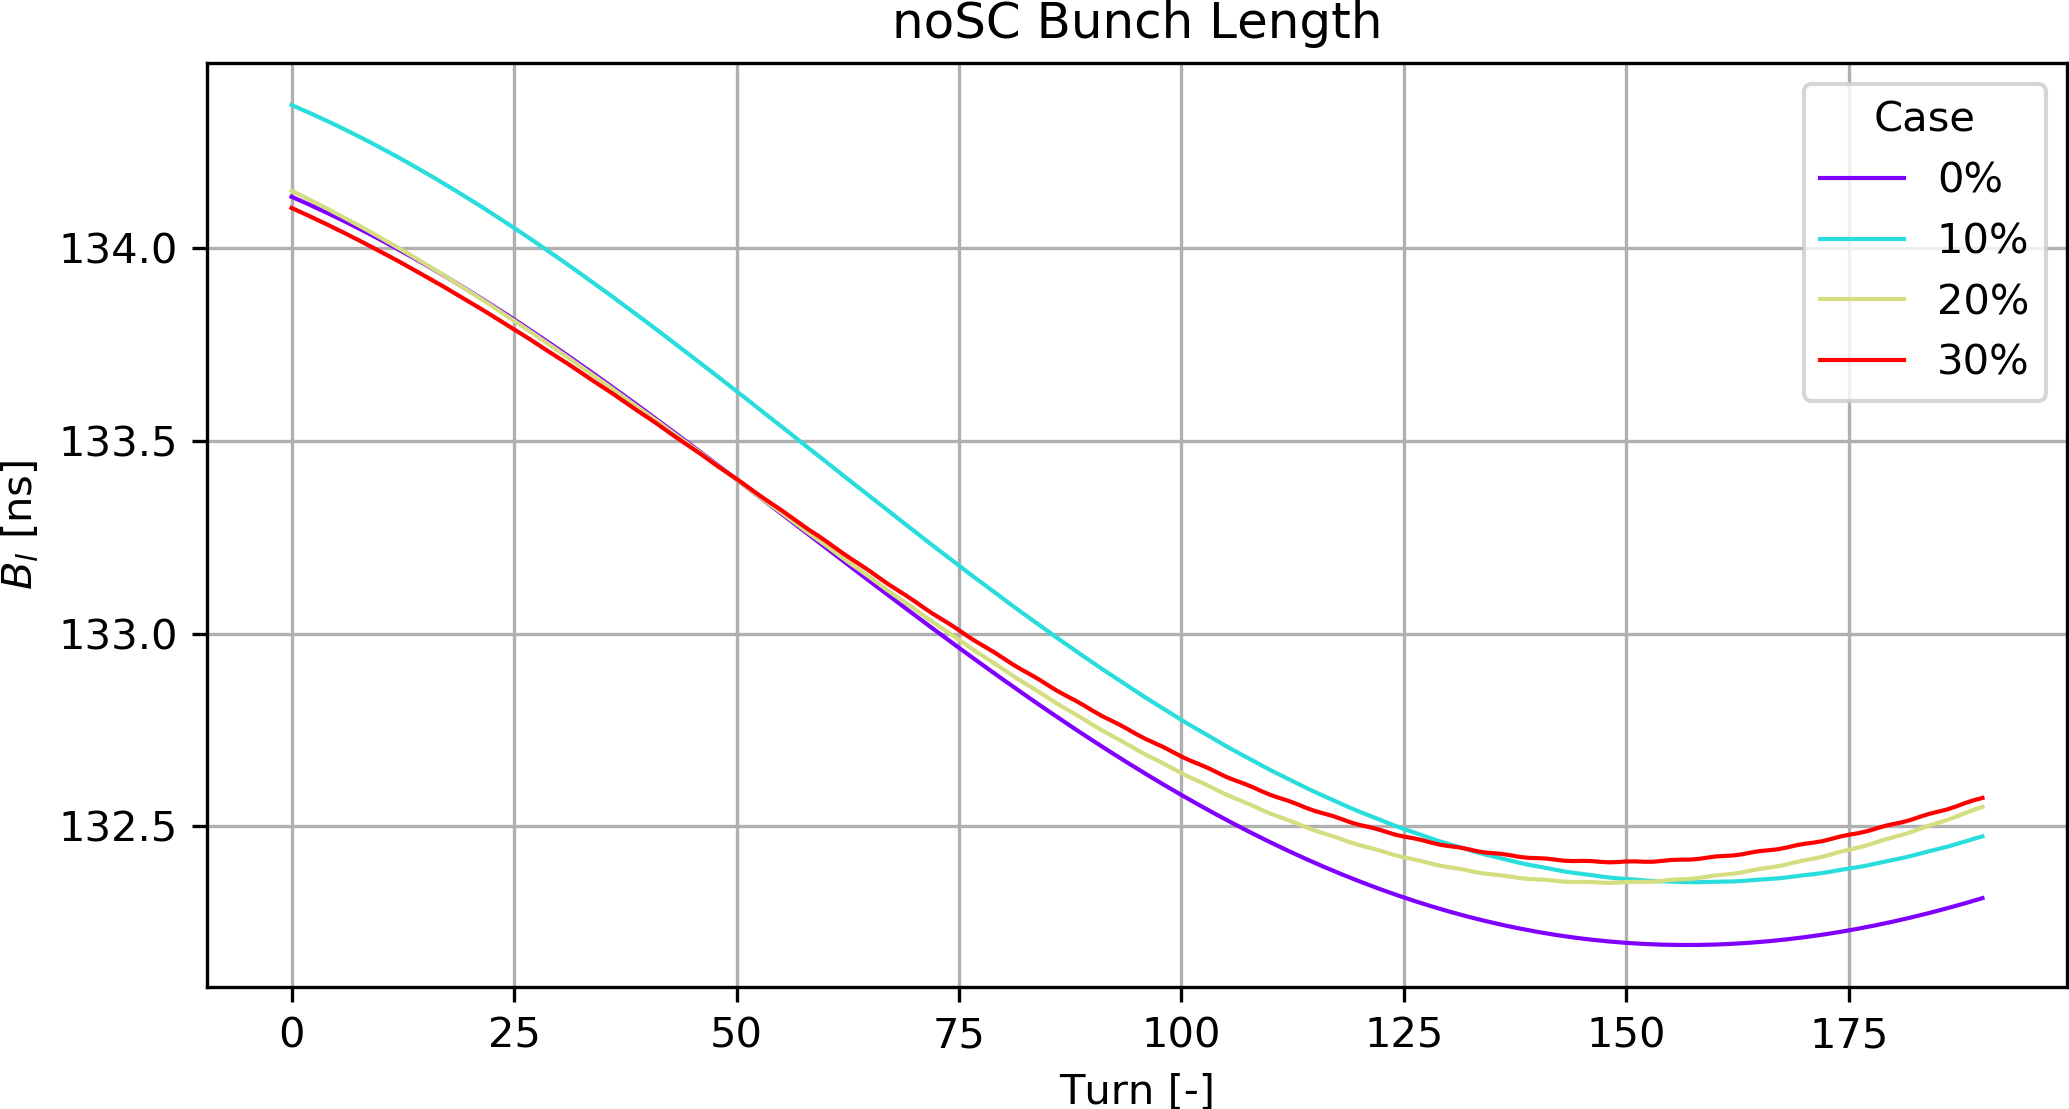
\includegraphics[width=0.45\textwidth]{PS_Transfer/NoSC/SEM_Tomo_noSC_bunchlength.png}~~~~
            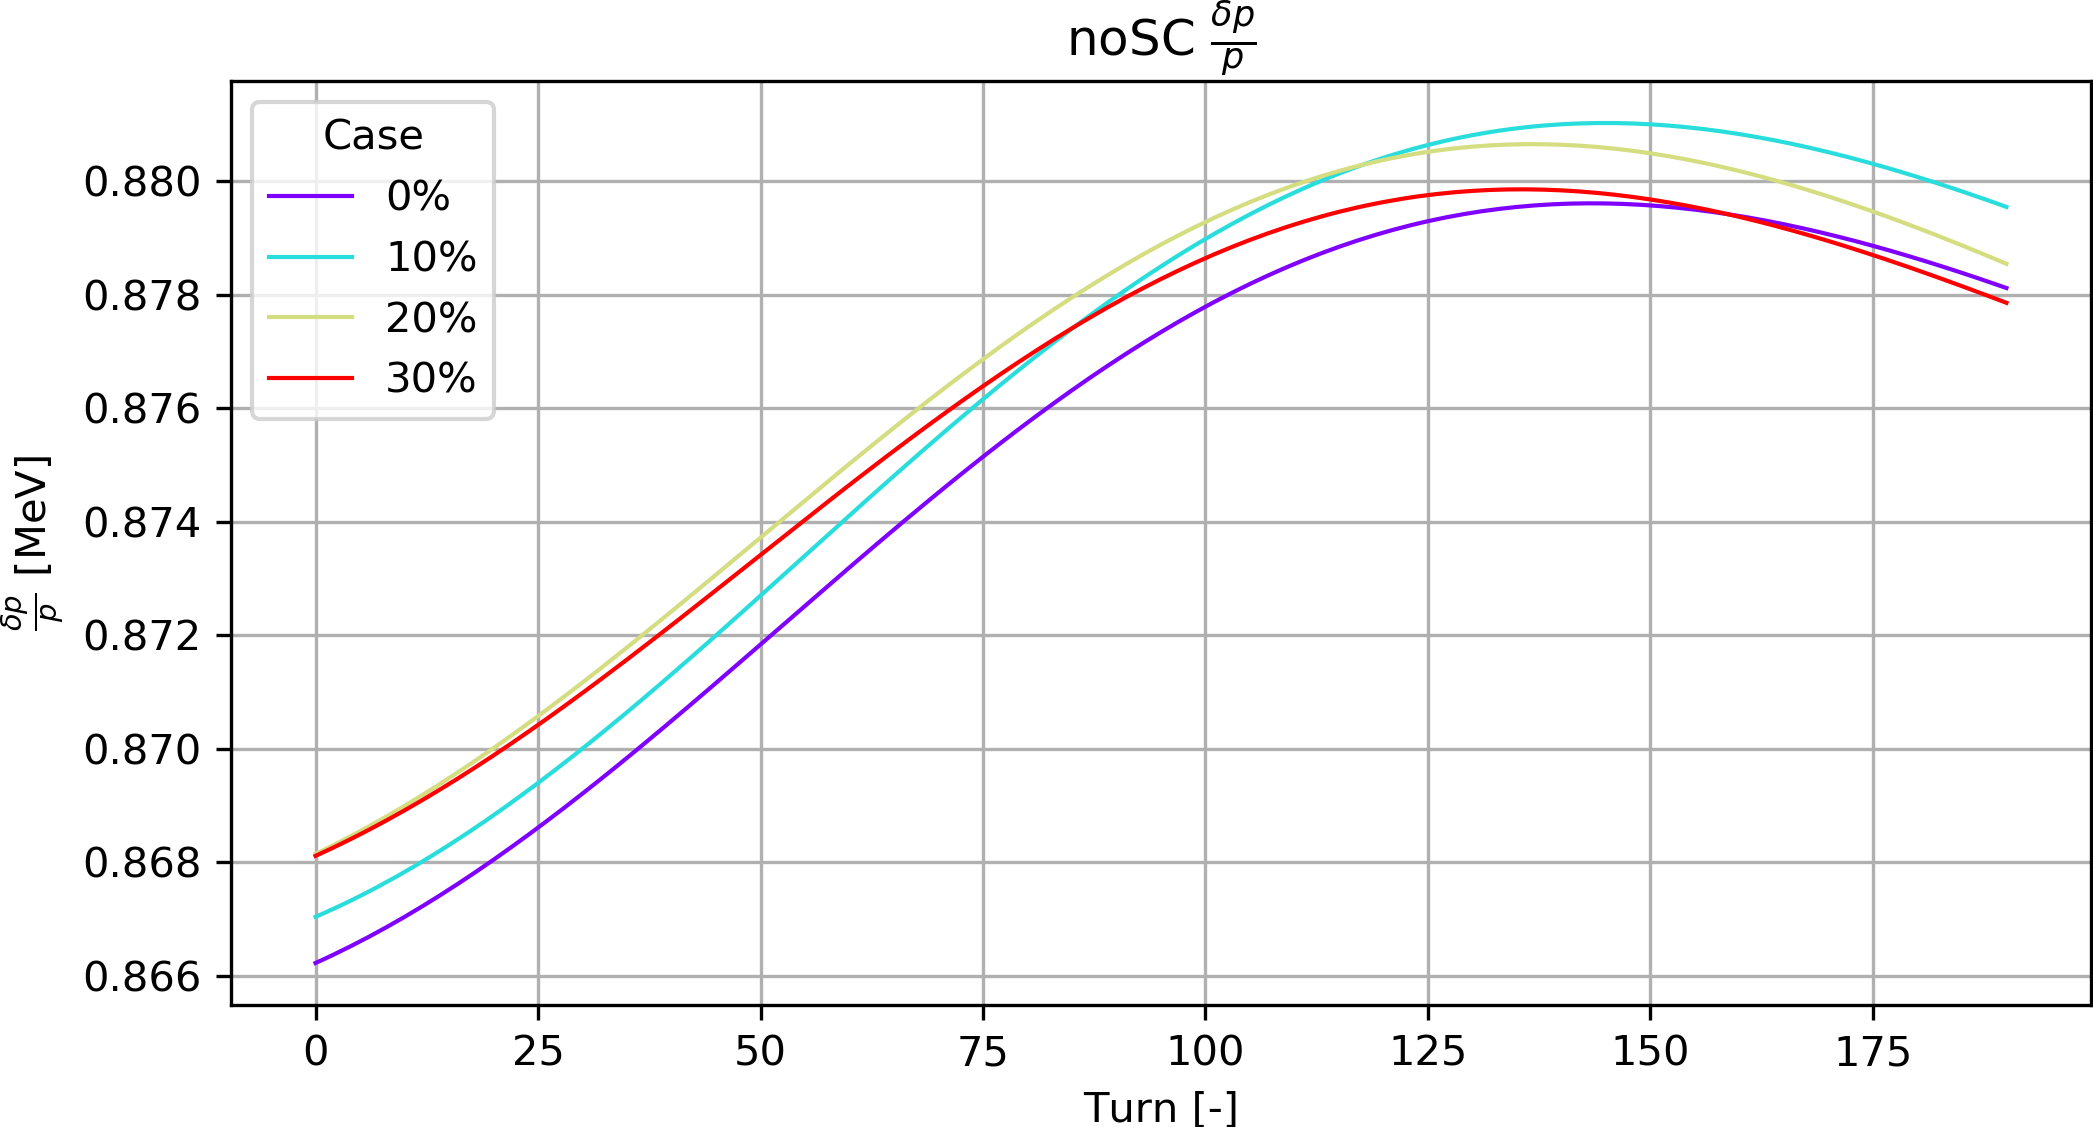
\includegraphics[width=0.45\textwidth]{PS_Transfer/NoSC/SEM_Tomo_noSC_dpp_rms.png}
            \caption{Longitudinal motion for \texttt{tomo} distribution: oscillation magnitude as expected.}
            \label{fig:tomo_longitudinal}
        \end{figure}
    }
    
    \frame{
        \frametitle{Tomo Distribution Horizontal Dispersion (No Space Charge)}
        
        \begin{figure}
            \centering
            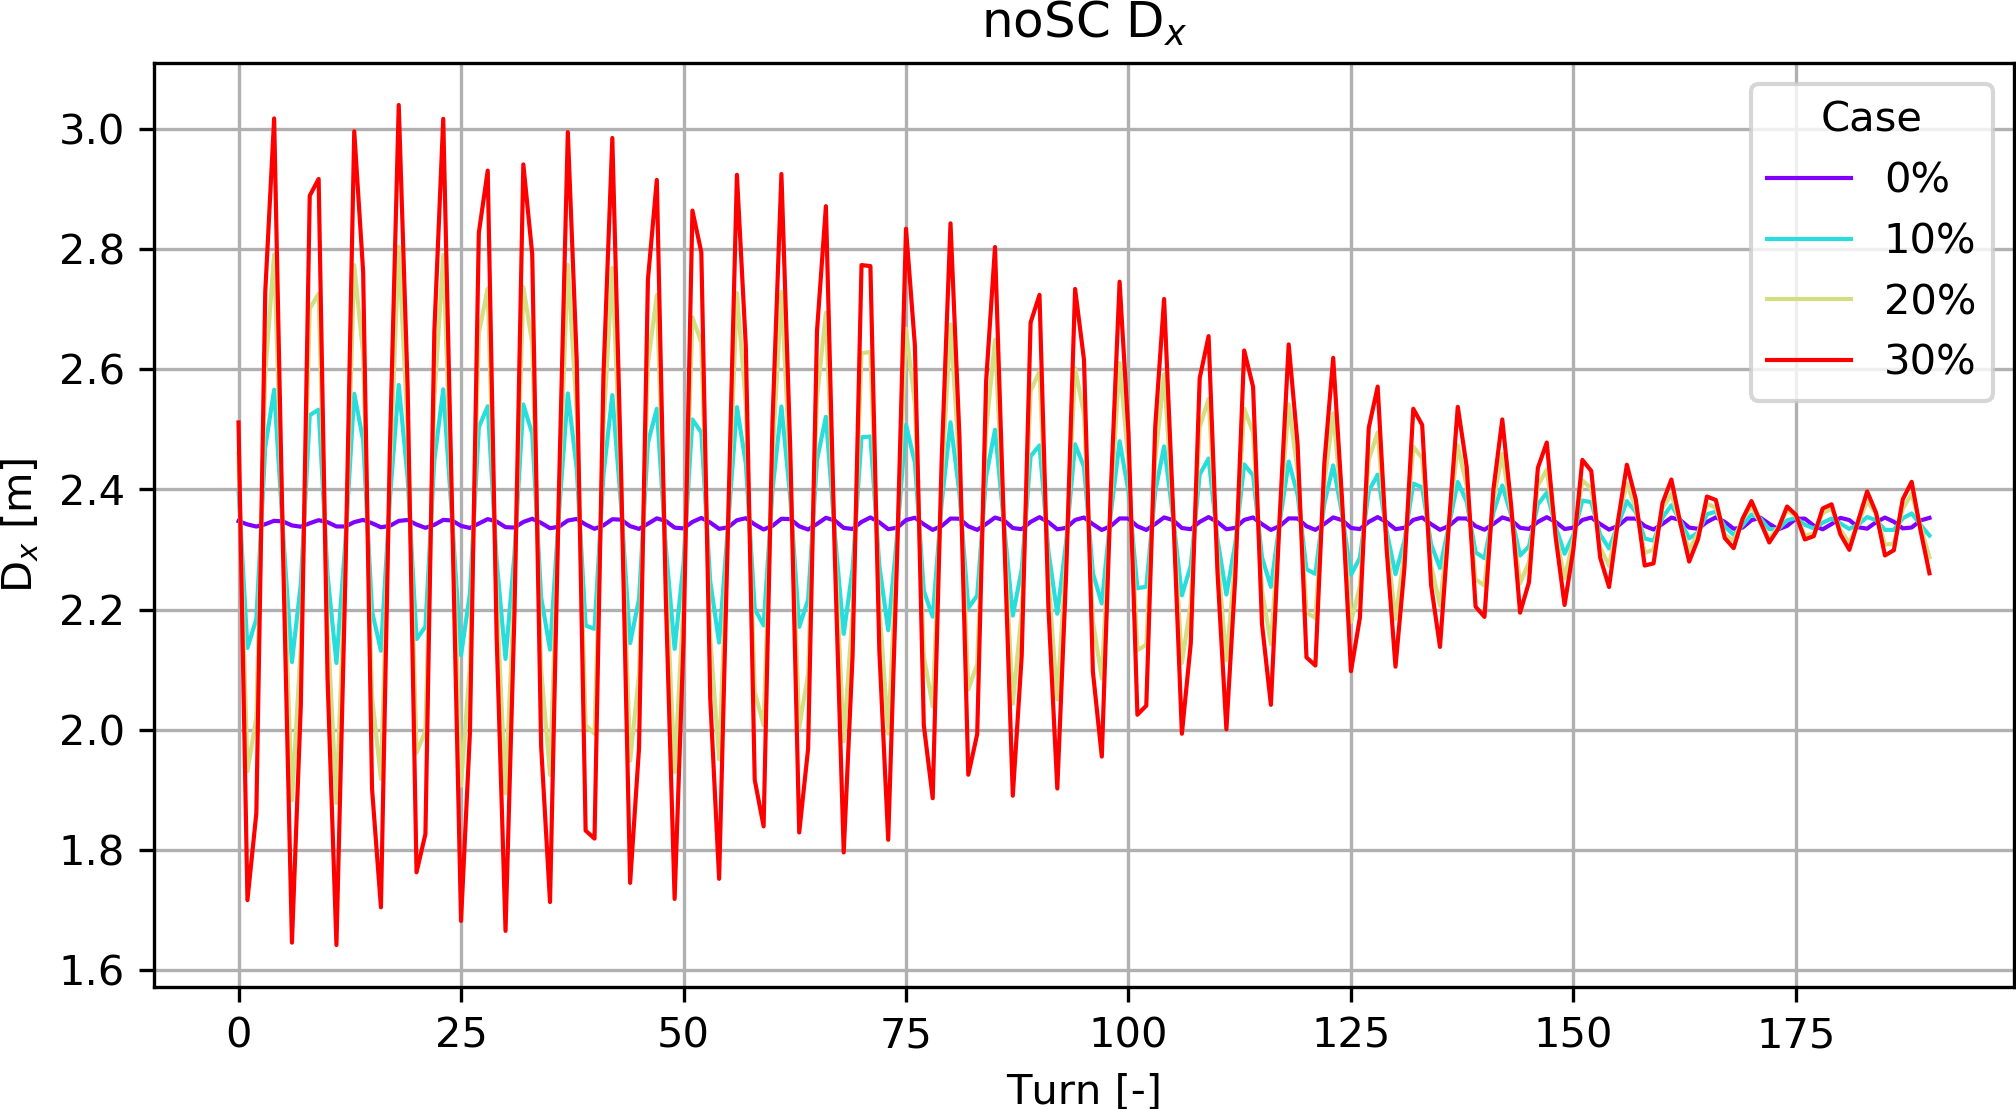
\includegraphics[width=0.45\textwidth]{PS_Transfer/NoSC/SEM_Tomo_noSC_D_x.png}~~~~
            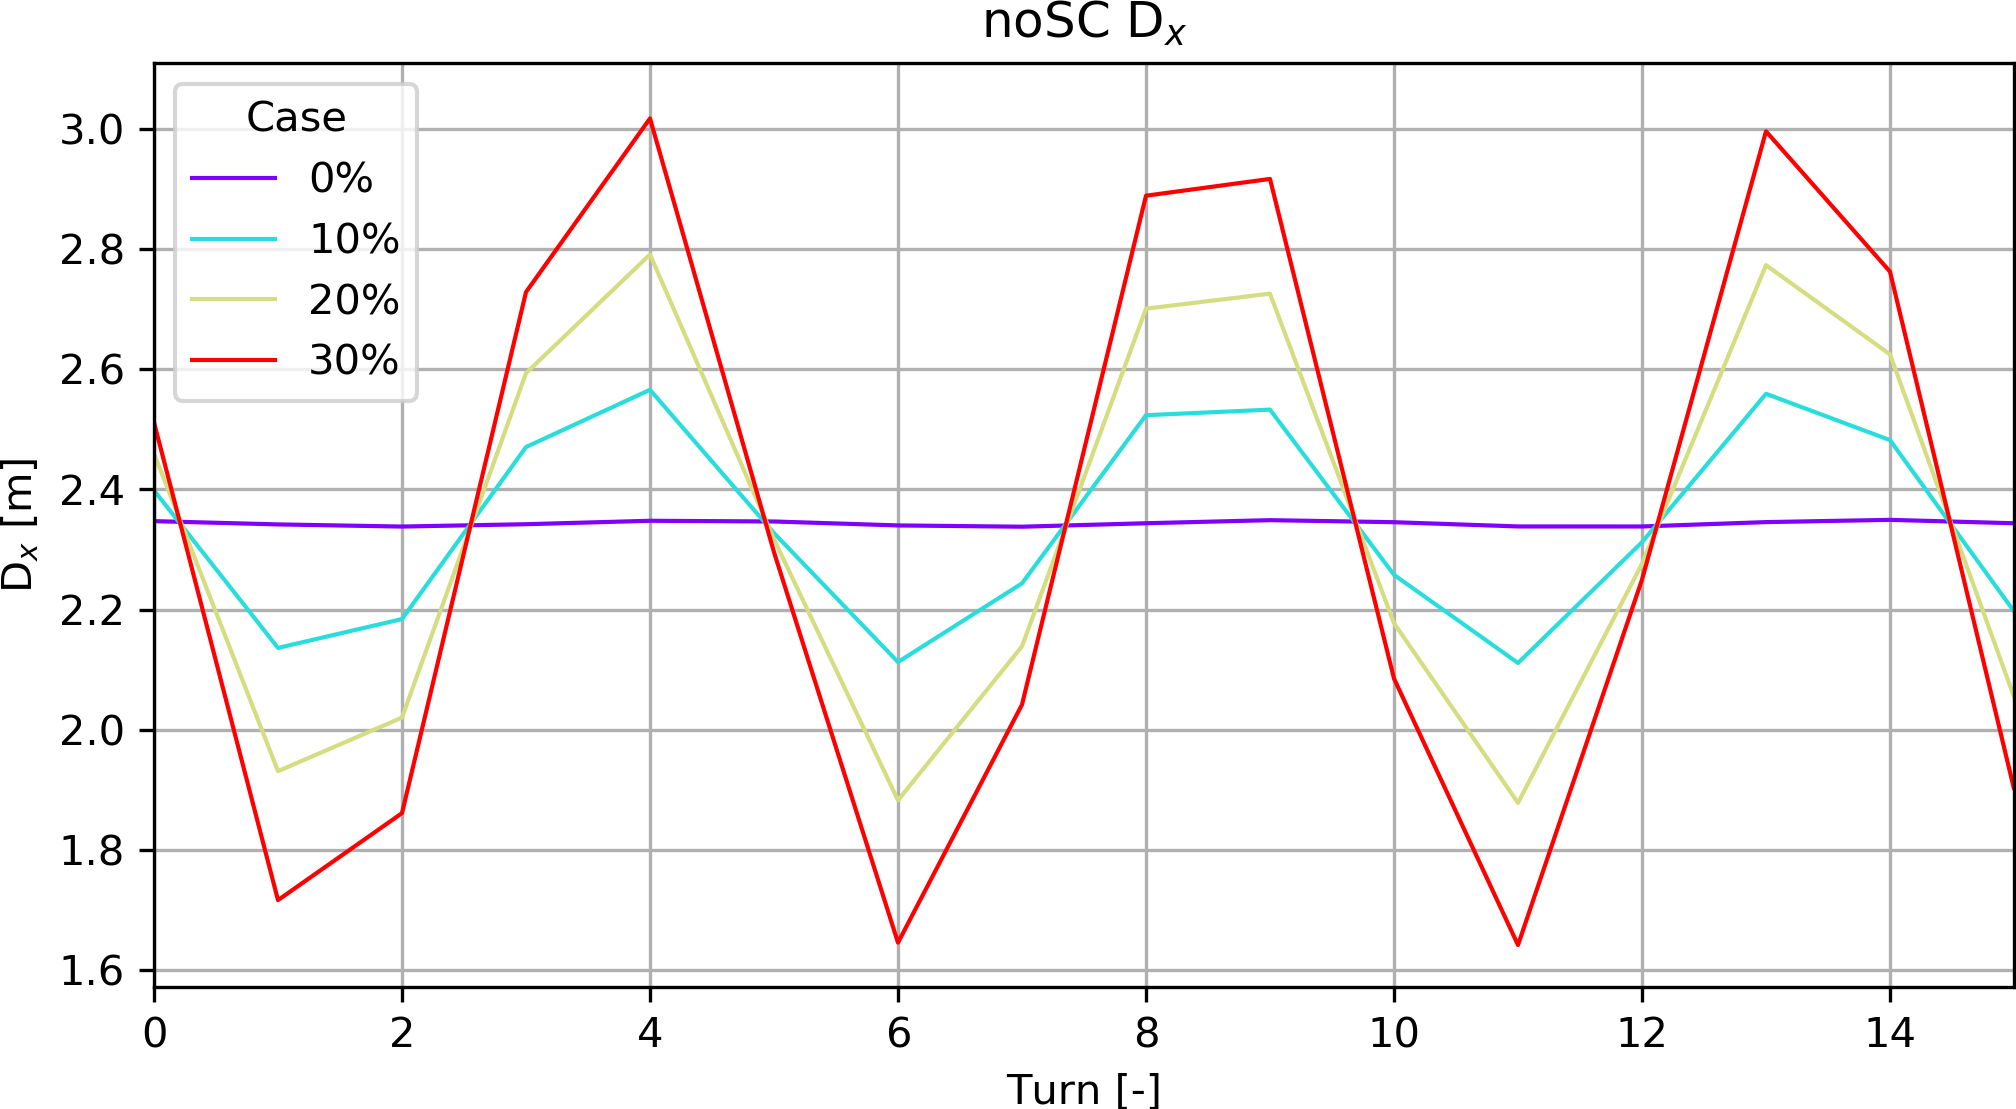
\includegraphics[width=0.45\textwidth]{PS_Transfer/NoSC/SEM_Tomo_noSC_zoom_D_x.png}
            \caption{Horizontal dispersion for \texttt{tomo} distribution: oscillation magnitude is a function of mismatch as expected.}
            \label{fig:tomo_dispersion}
        \end{figure}
    }
    
    \frame{
        \frametitle{Tomo Distribution Emittances (No Space Charge)}
        
        \begin{figure}
            \centering
            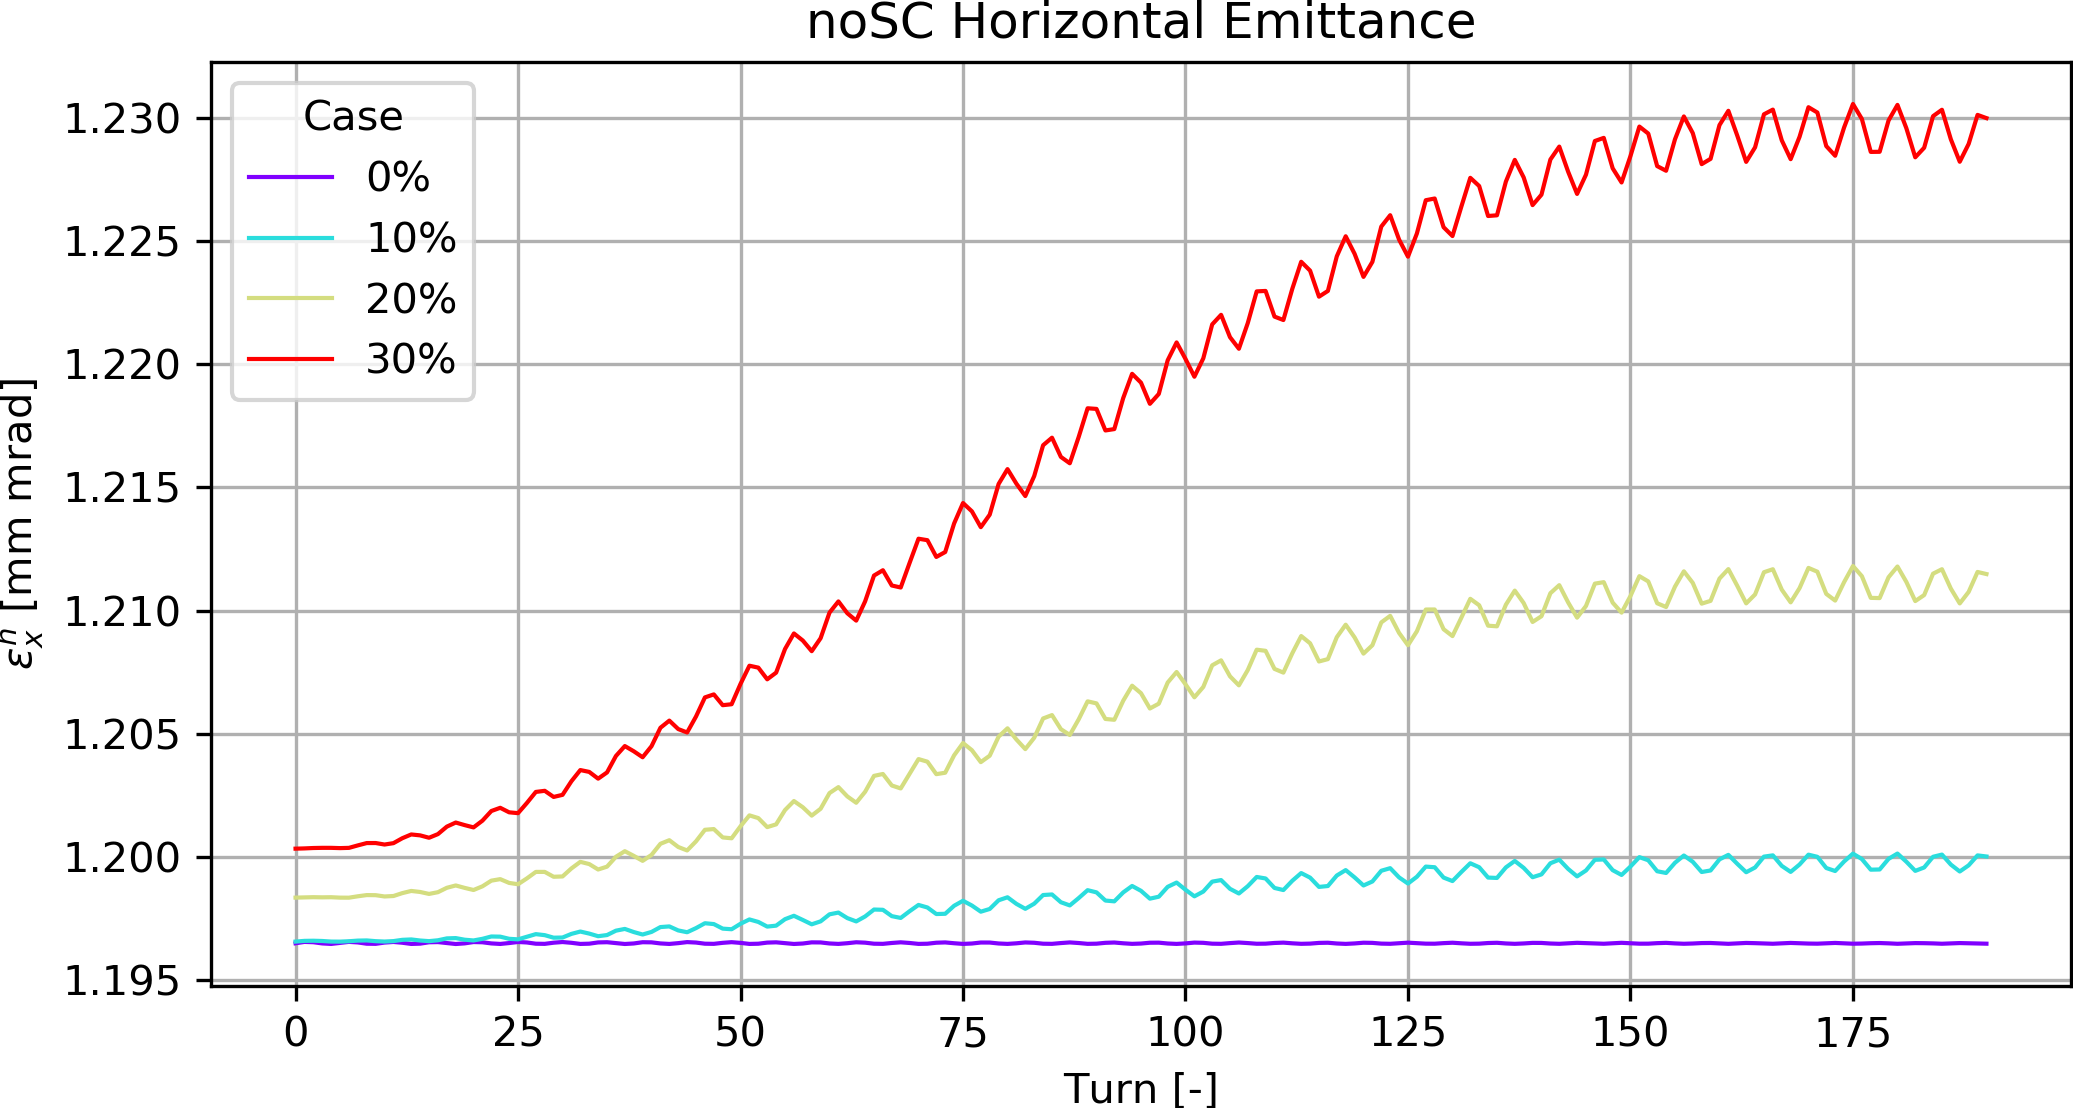
\includegraphics[width=0.45\textwidth]{PS_Transfer/NoSC/SEM_Tomo_noSC_epsn_x.png}~~~~
            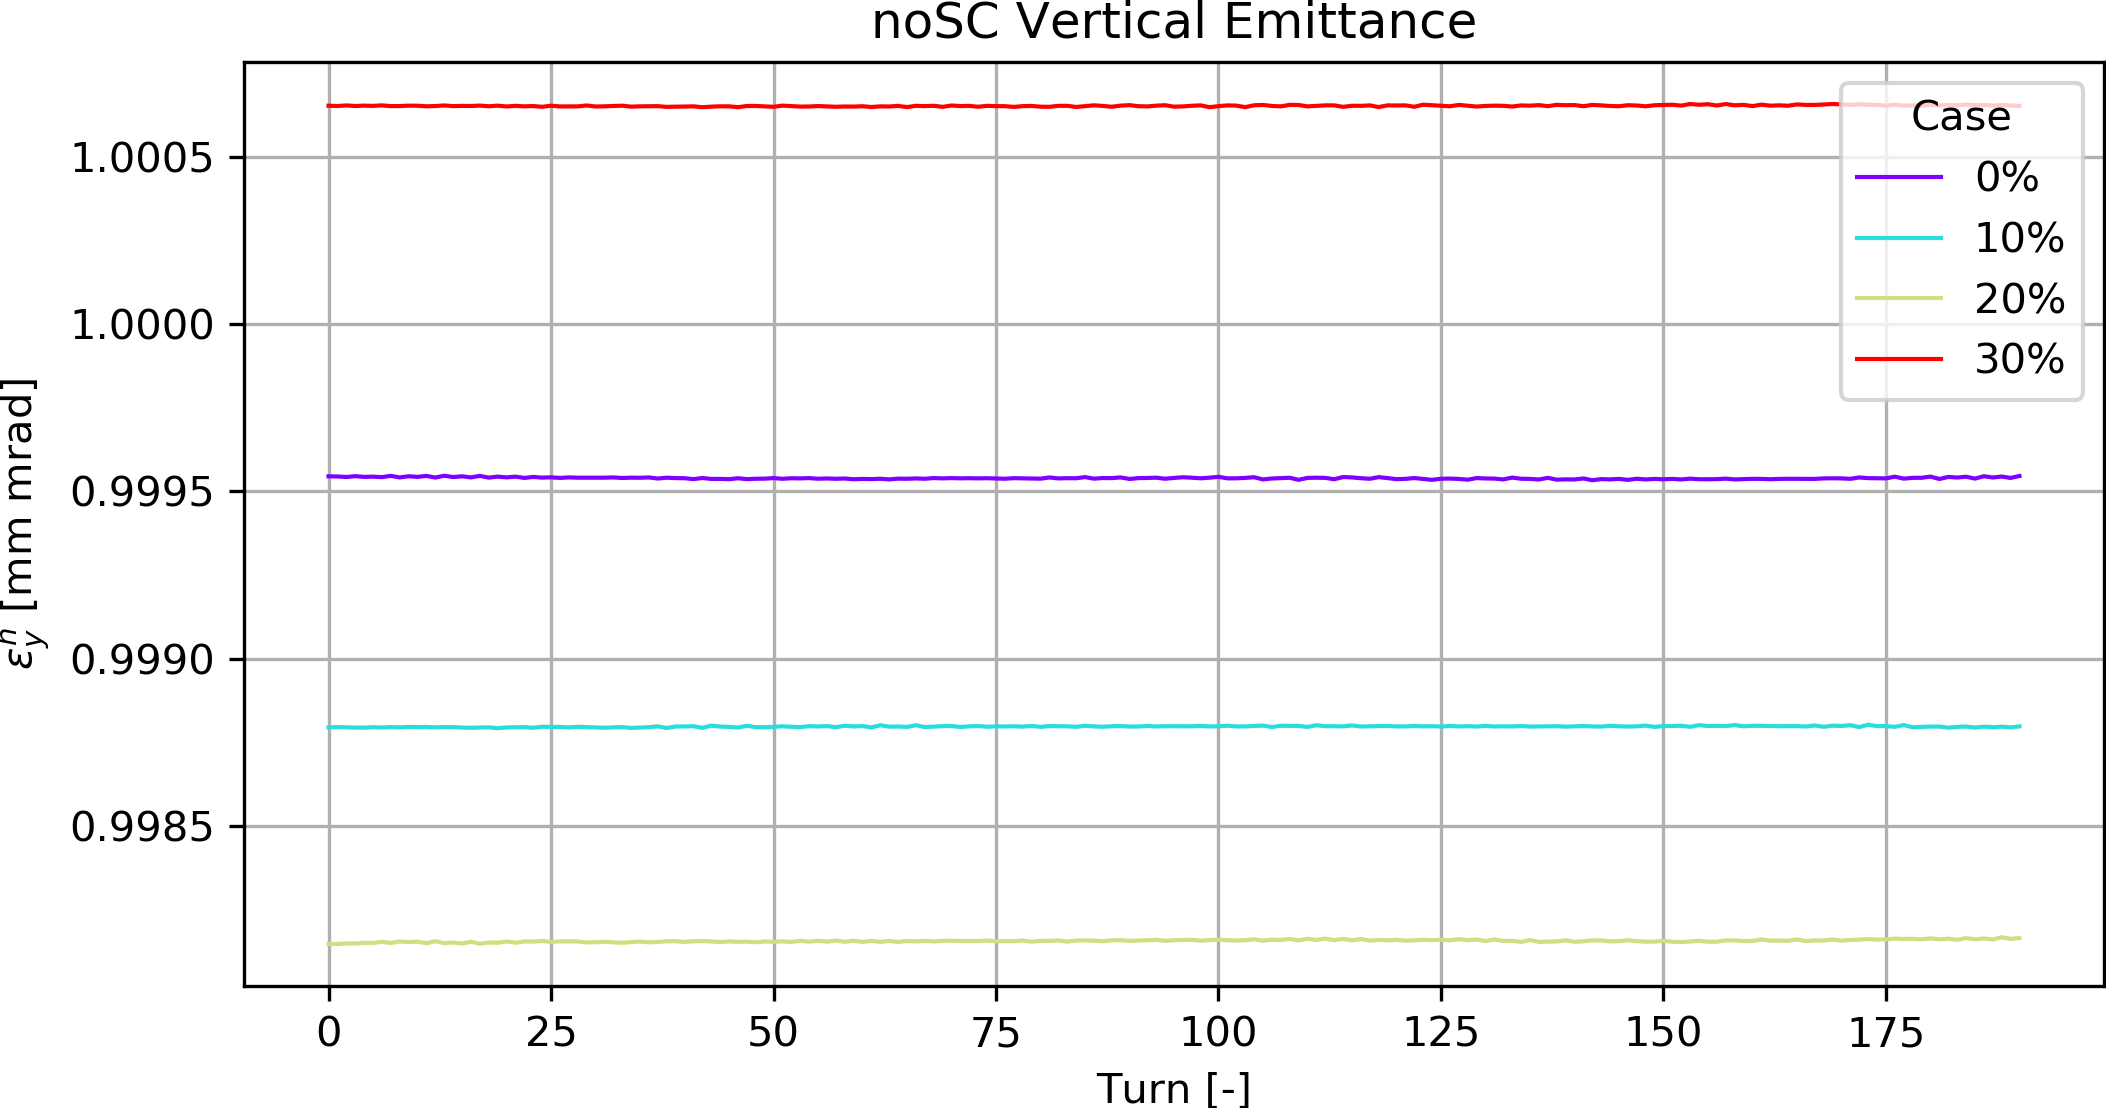
\includegraphics[width=0.45\textwidth]{PS_Transfer/NoSC/SEM_Tomo_noSC_epsn_y.png}
            \caption{Emittances for \texttt{tomo} distribution: horizontal emittance growth is a function of dispersion mismatch.}
            \label{fig:tomo_emittances}
        \end{figure}
    }
    
    \frame{
        \frametitle{Tomo Distribution}
        \begin{block}{With Space Charge} Mismatch of factor +10\%, +20\%, and +30\%.
        \end{block}
    }
    
     \frame{
        \frametitle{Tomo Distribution Longitudinal Motion (With Space Charge)}
        
        \begin{figure}
            \centering
            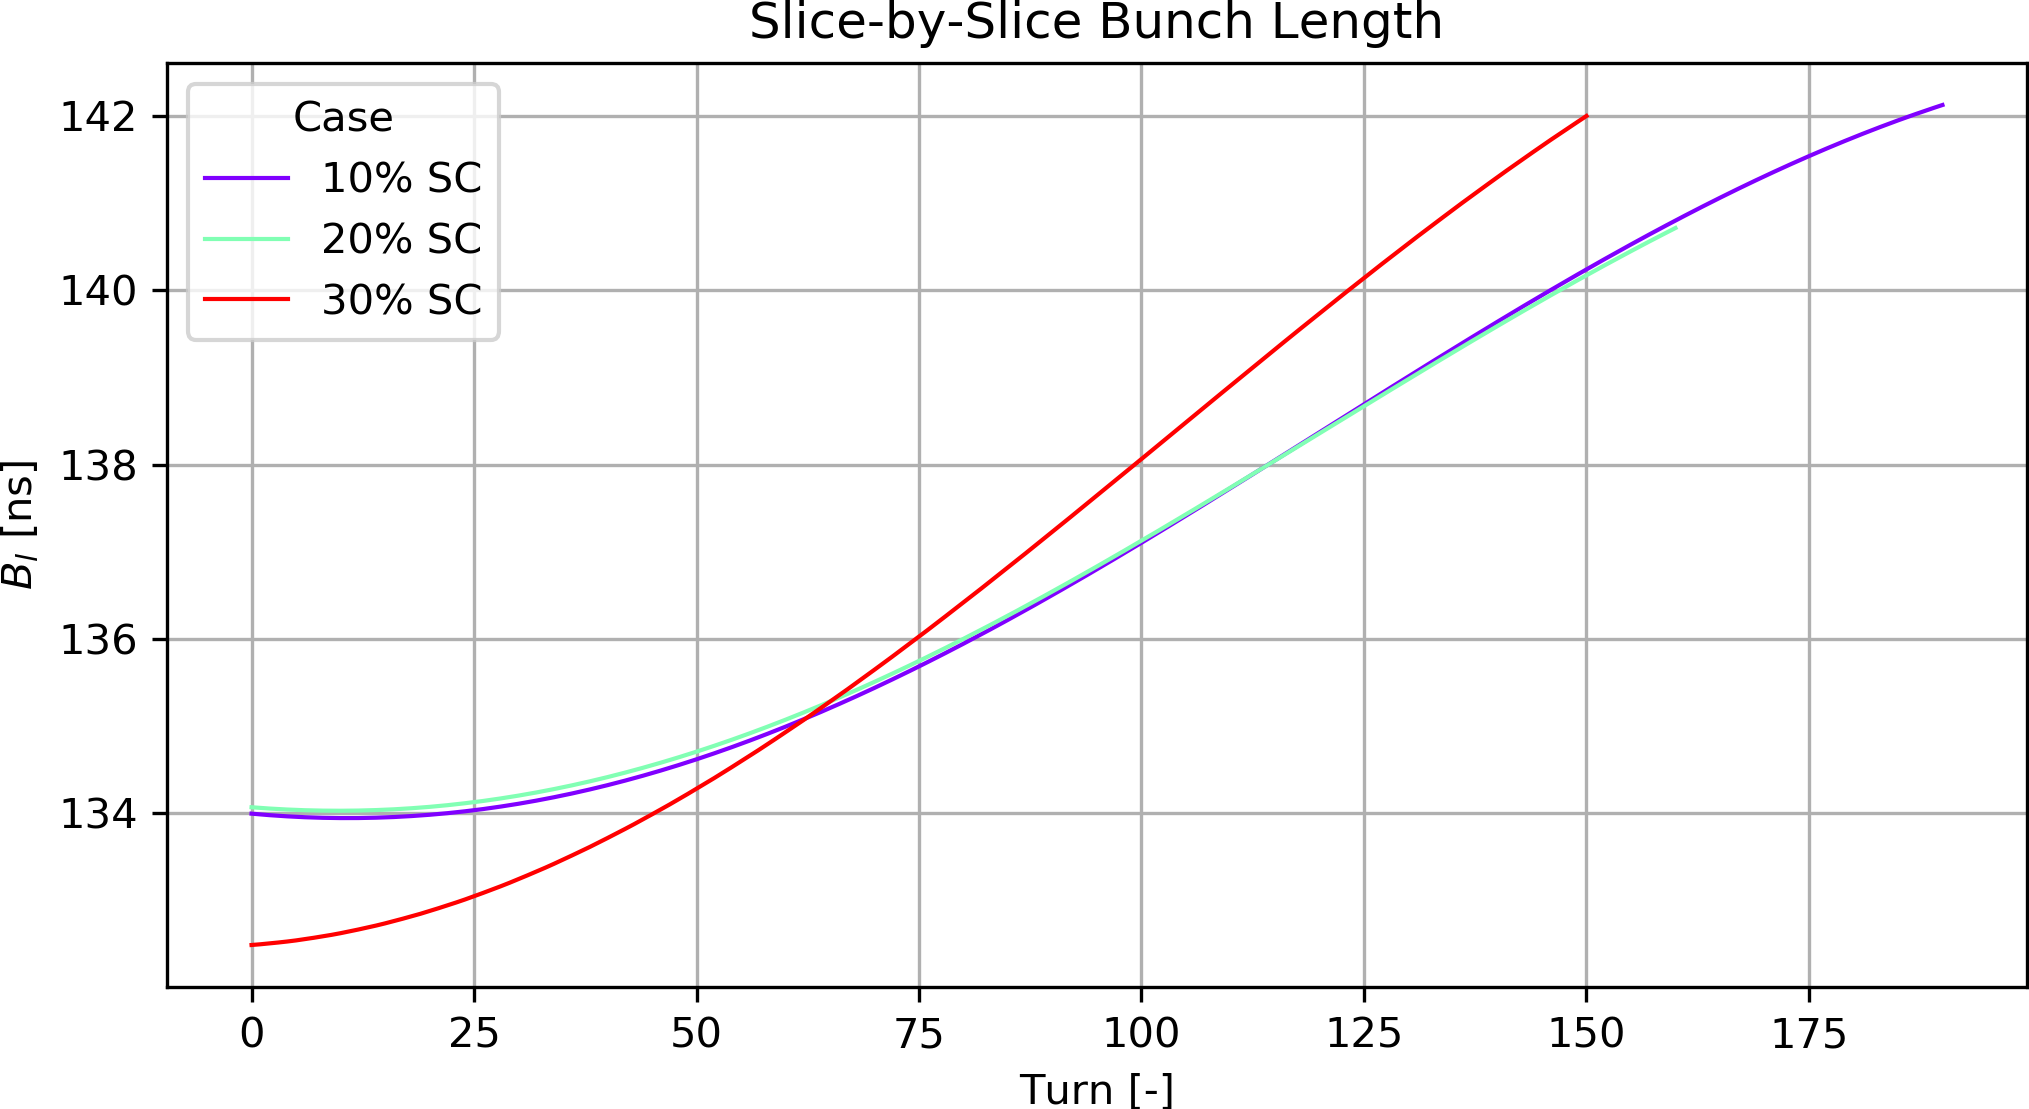
\includegraphics[width=0.45\textwidth]{PS_Transfer/SC/SEM_Tomo_bunchlength.png}~~~~
            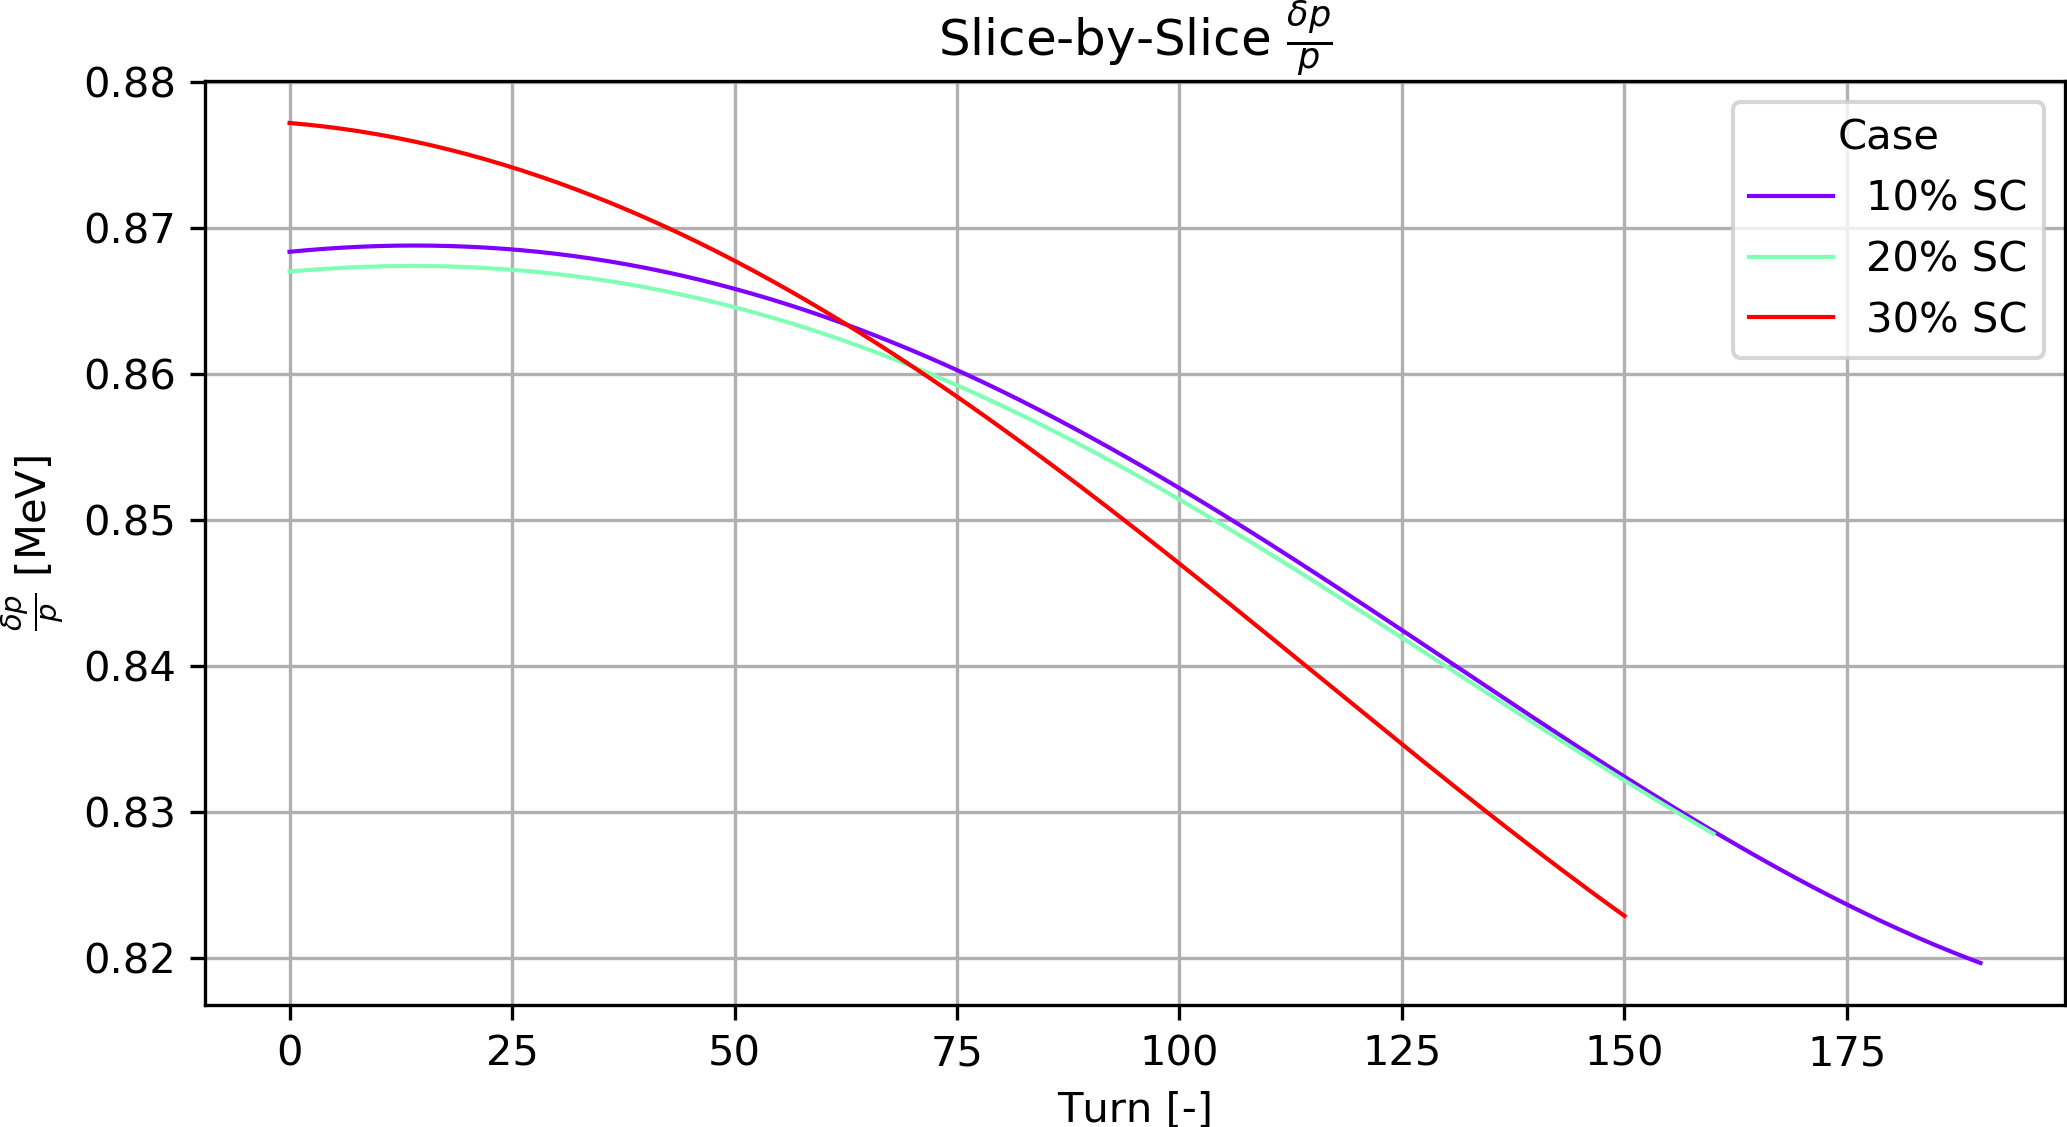
\includegraphics[width=0.45\textwidth]{PS_Transfer/SC/SEM_Tomo_dpp_rms.png}
            \caption{Longitudinal motion for \texttt{tomo} distribution with space charge: oscillation has opposite sign to no space charge case - SC drives bunch lengthening at the start?}
            \label{fig:tomo_longitudinal}
        \end{figure}
    }
    
    \frame{
        \frametitle{Tomo Distribution Horizontal Dispersion (With Space Charge)}
        
        \begin{figure}
            \centering
            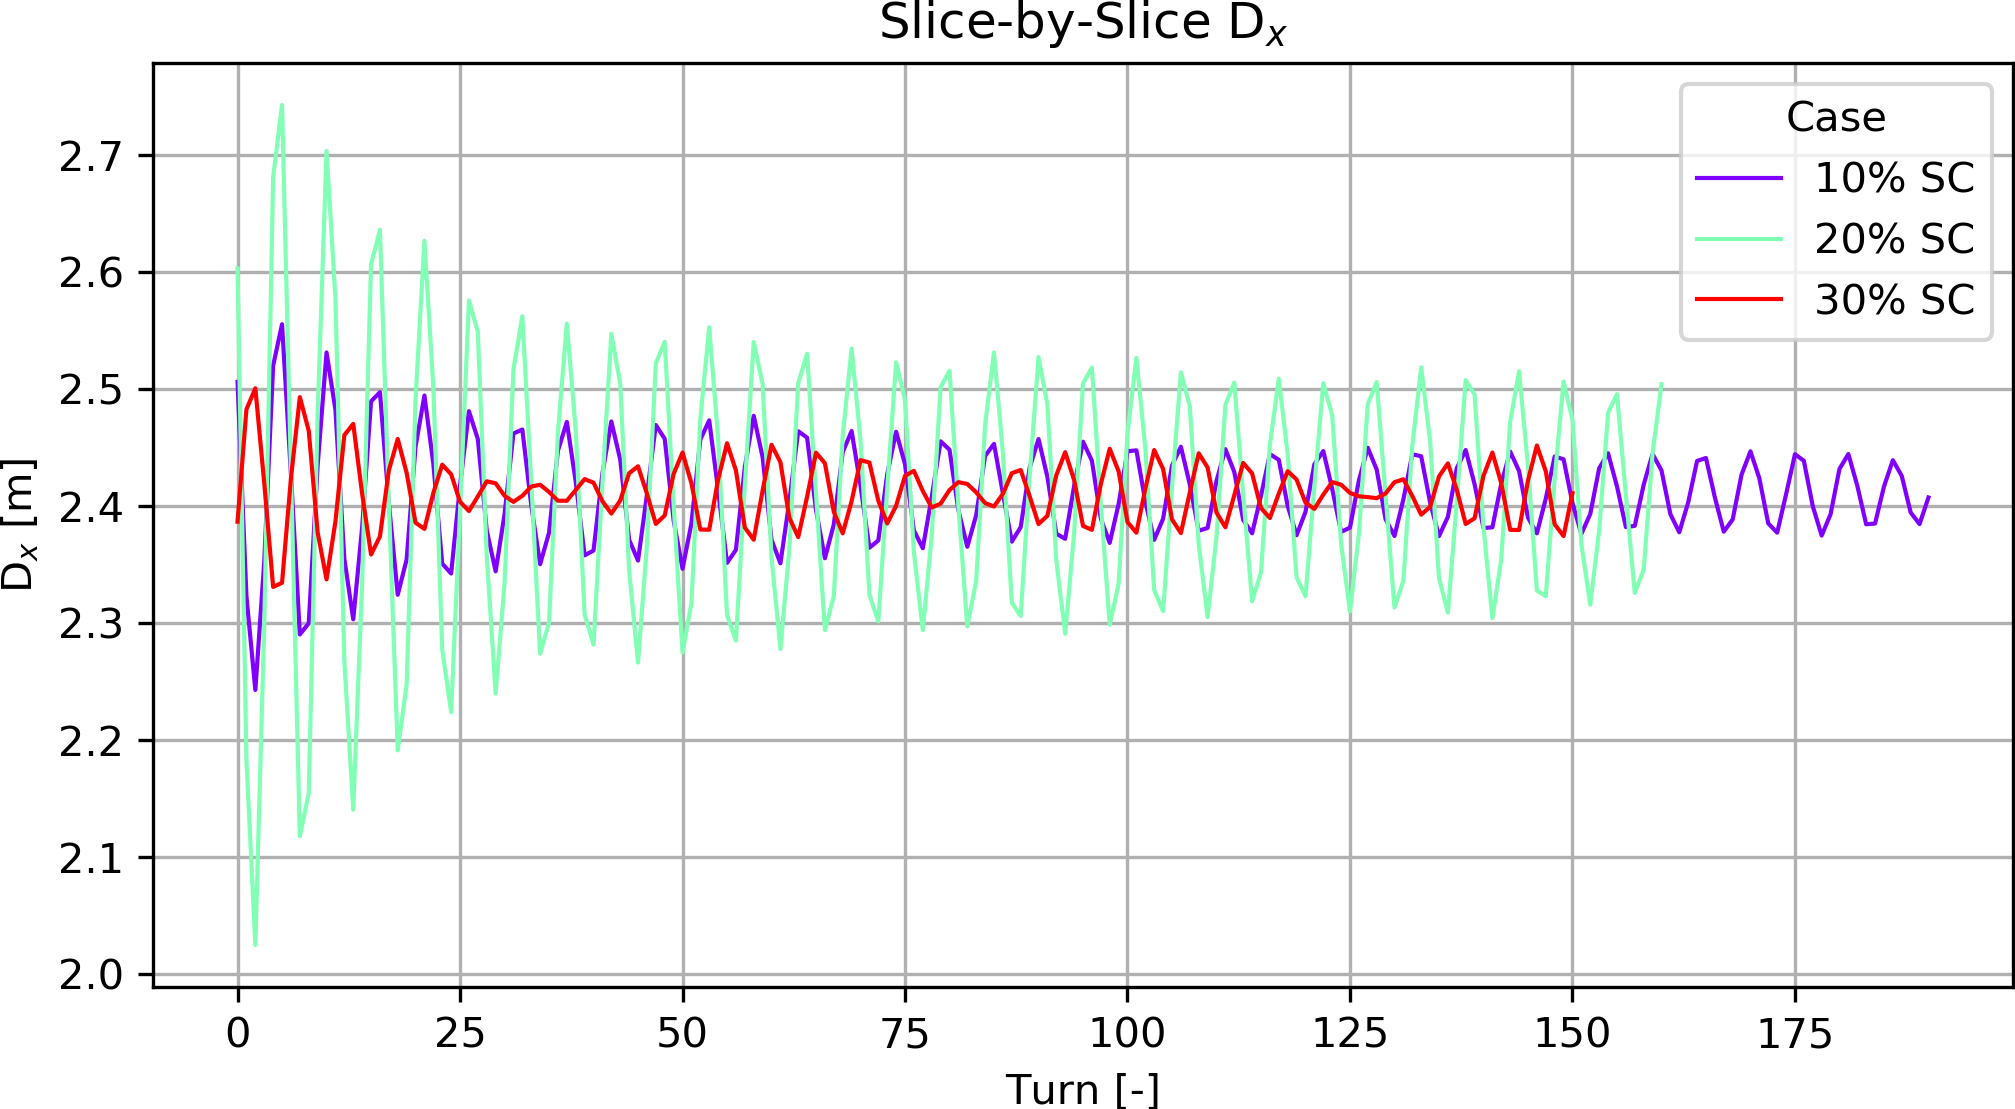
\includegraphics[width=0.45\textwidth]{PS_Transfer/SC/SEM_Tomo_D_x.png}~~~~
            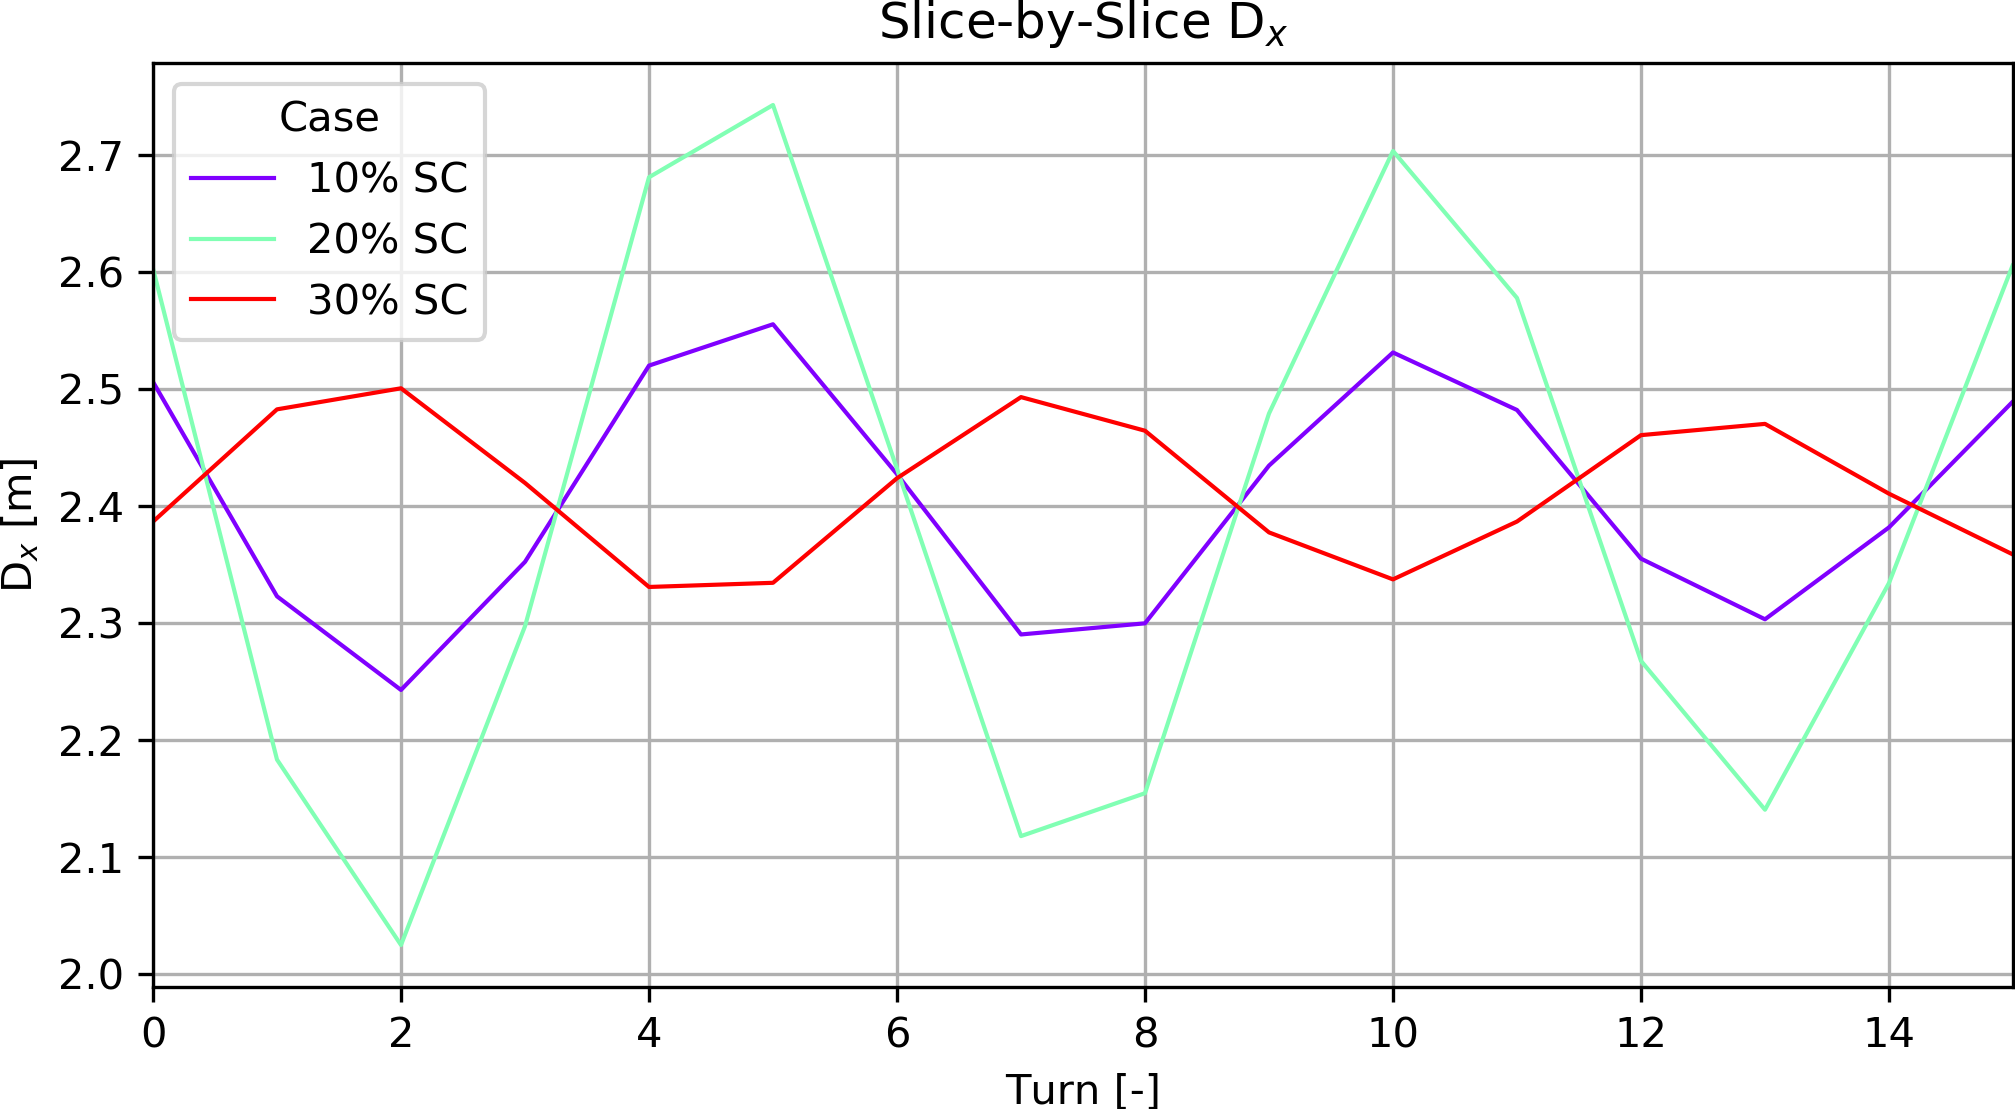
\includegraphics[width=0.45\textwidth]{PS_Transfer/SC/SEM_Tomo_zoom_D_x.png}
            \caption{Horizontal dispersion for \texttt{tomo} distribution with space charge: dispersion oscillations have longer period, highest mismatch in anti-phase rather than larger magnitude.}
            \label{fig:tomo_dispersion}
        \end{figure}
    }
    
    \frame{
        \frametitle{Tomo Distribution Emittances (With Space Charge)}
        
        \begin{figure}
            \centering
            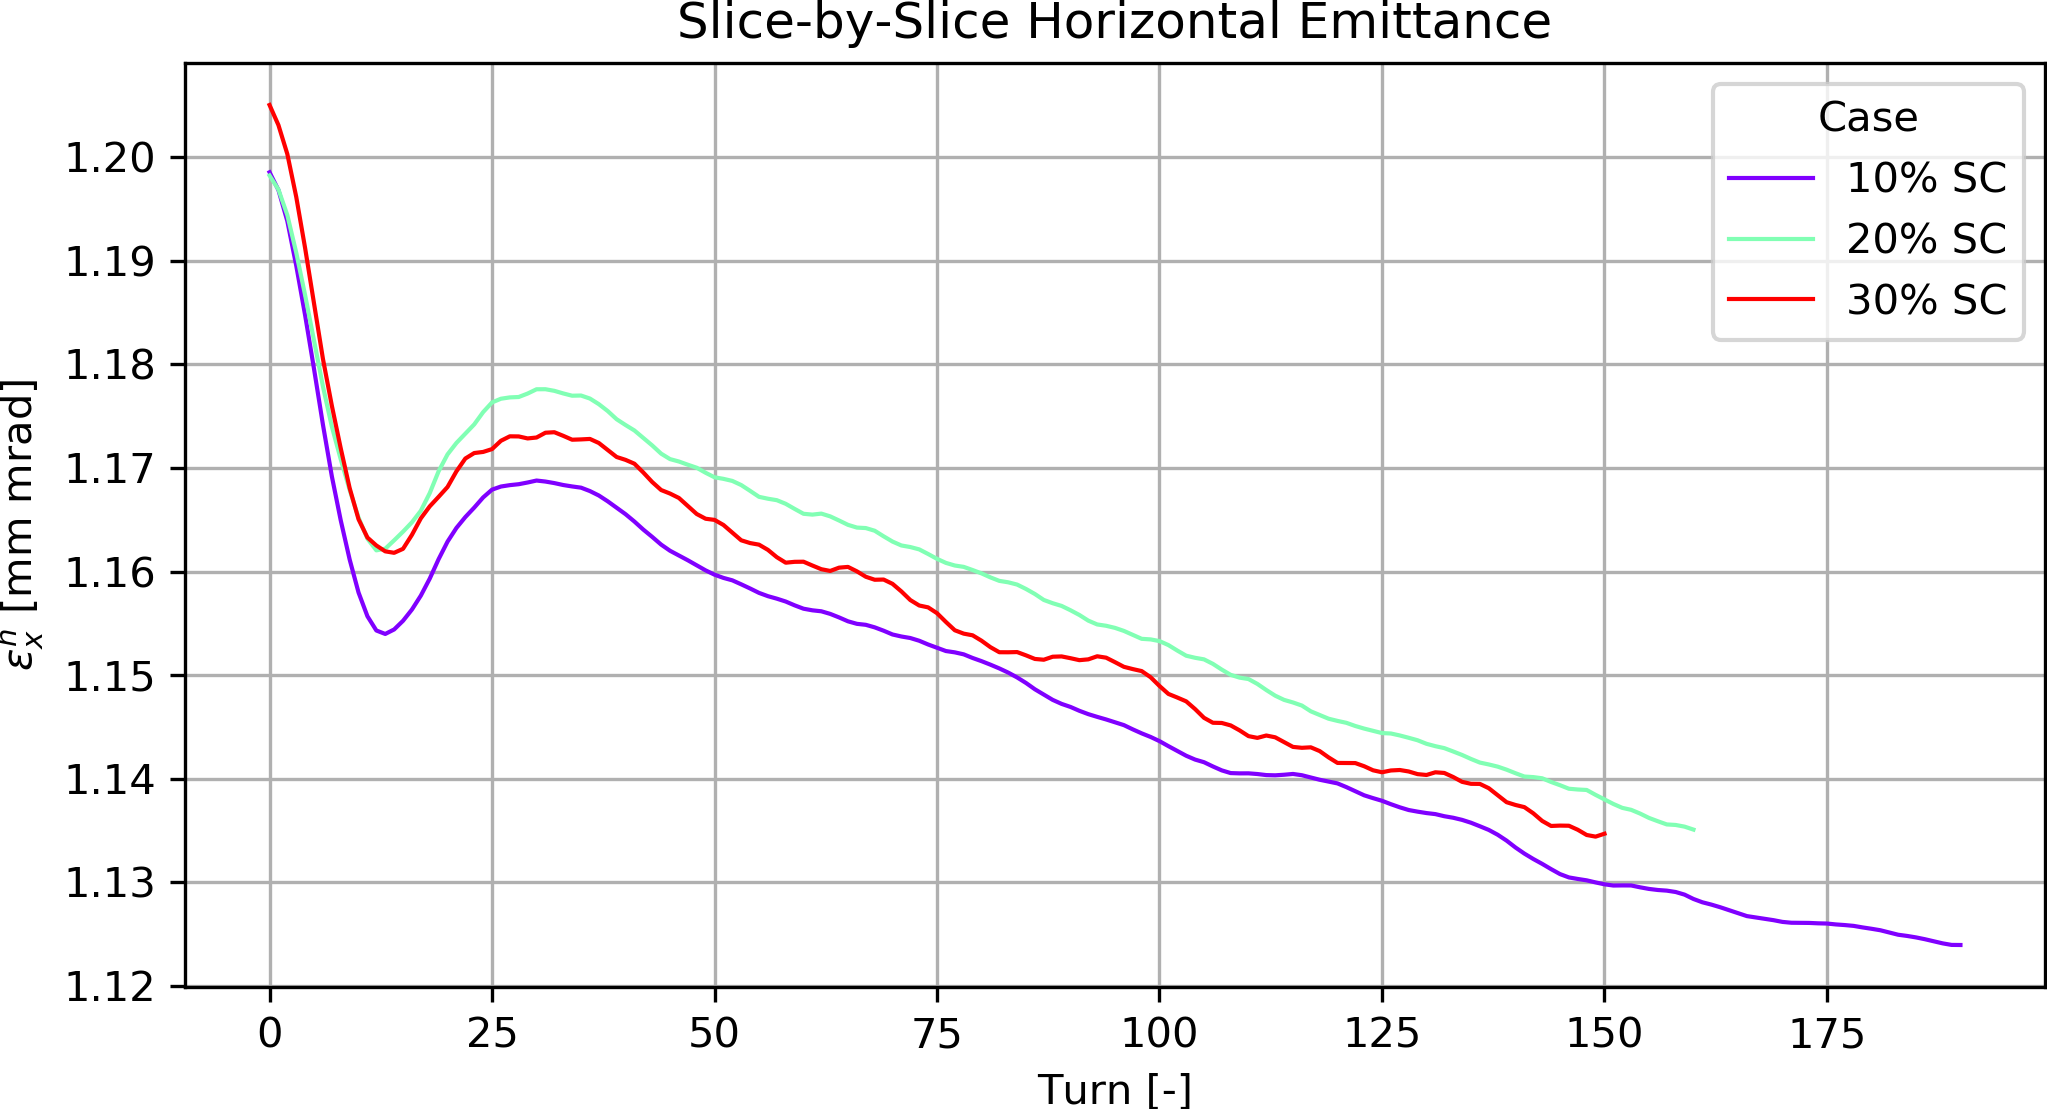
\includegraphics[width=0.45\textwidth]{PS_Transfer/SC/SEM_Tomo_epsn_x.png}~~~~
            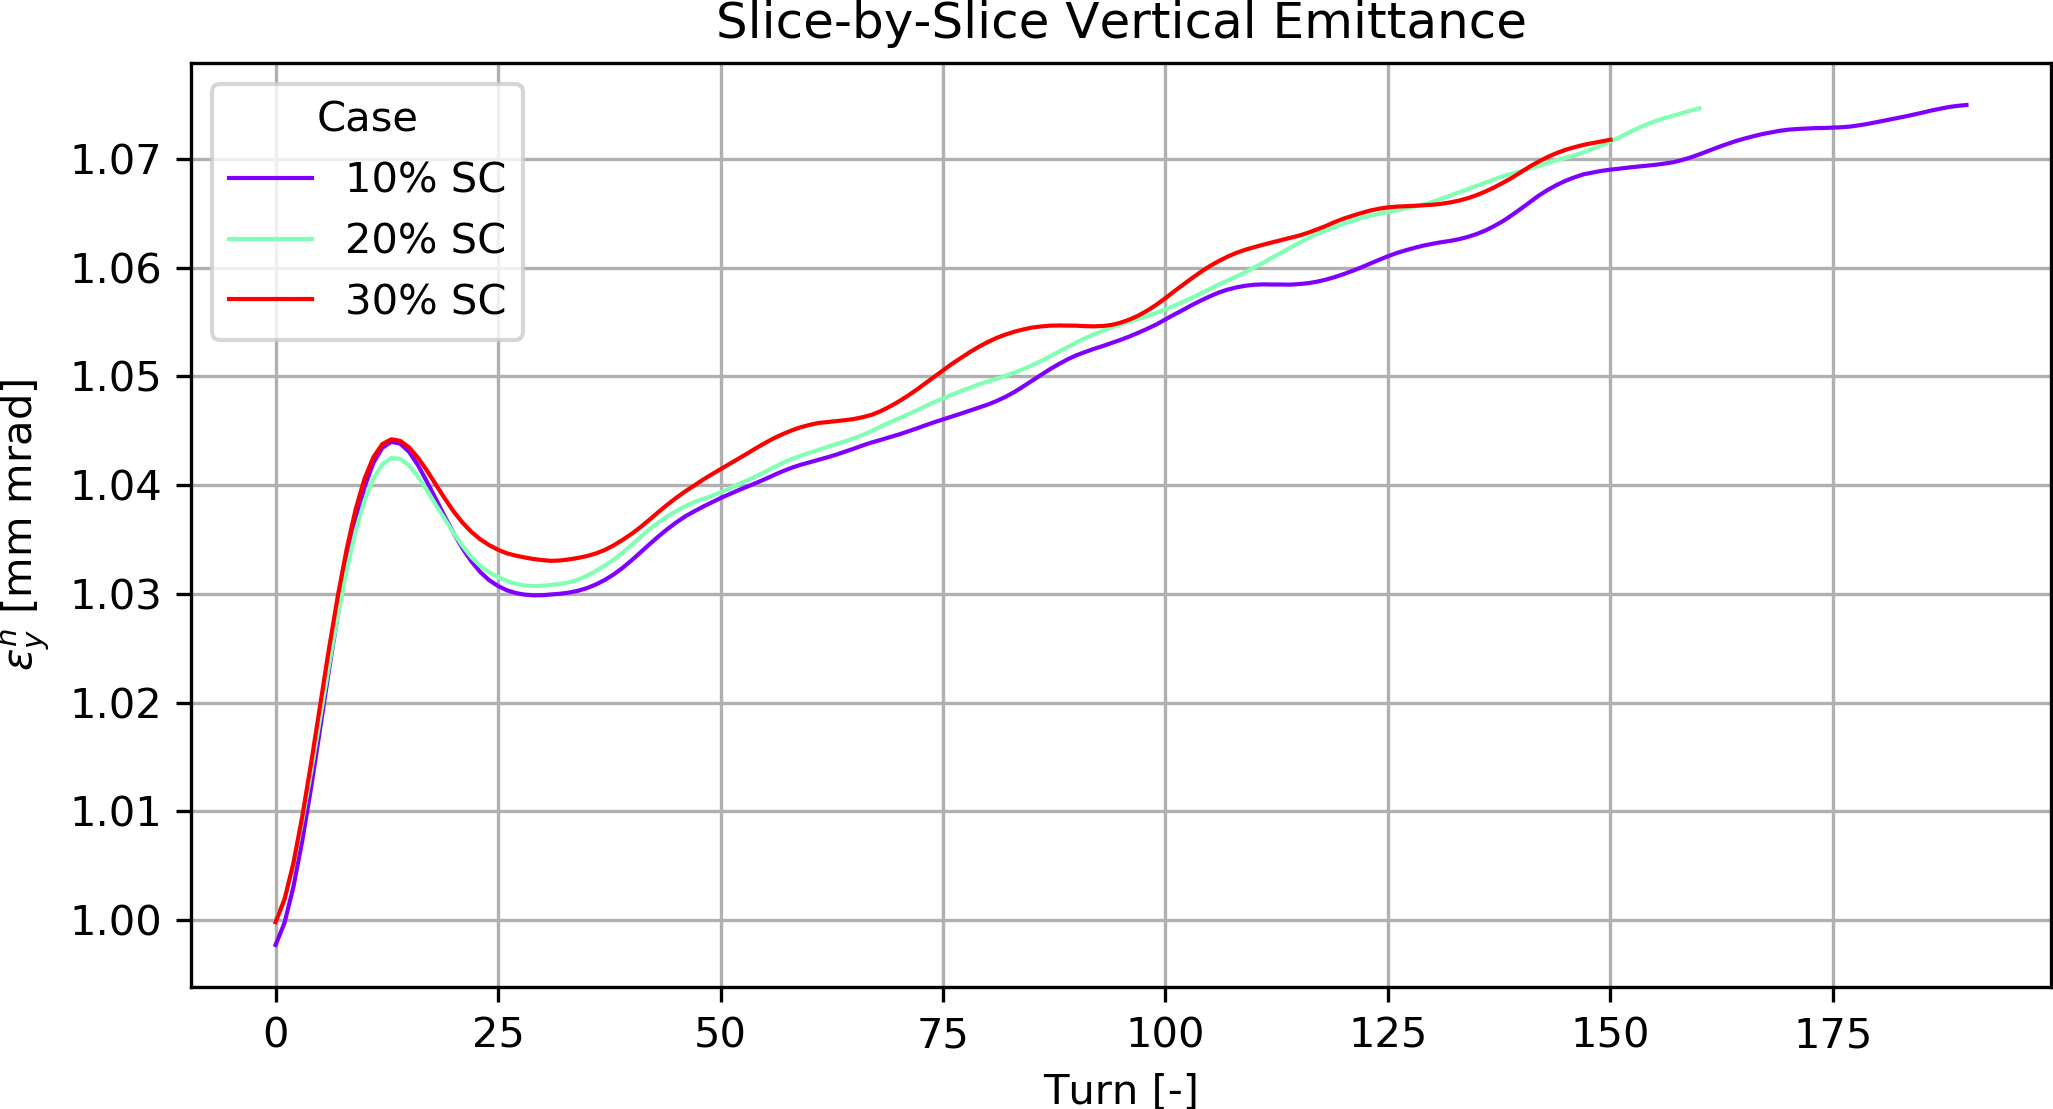
\includegraphics[width=0.45\textwidth]{PS_Transfer/SC/SEM_Tomo_epsn_y.png}
            \caption{Emittances for \texttt{tomo} distribution with space charge: clear emittance exchange.}
            \label{fig:tomo_emittances}
        \end{figure}
    }
    
    
    
    \cernSplashWhite

\end{document}

